\newchapter{Szenen}

\newsection{Prolog (optional)}

Um die Ermittler auf den Plot, ihren Charakter und auf die vorherrschenden politischen Gemengelage vorzubereiten, bietet es sich an mit jedem der Spieler einzeln eine Einf"uhrungsrunde zu spielen.

Der Vertraute des \underline{Cynarian Chefermittlers} ist Colonel Scholz. Er wird den Chefermittler auf das Treffen mit Vandermool, mit dem der Ermittler selbst noch nicht viel zu tun hatte, einweisen. Vandermool ist auf ein gutes Verh"altnis mit dem Protektorat bem"uht wird aber bei einer Zusammenarbeit die F"uhrung behalten. Zudem ist nicht klar ob die Mutanten in die Anschl"age verwickelt sind oder evtl. ~sogar Cynarian selbst deshalb ist Vorsicht geboten.

\underline{Für den Assistenten} bietet sich eine Einweisung in T"atigkeit als Psychonaut an und ihn dabei gleich direkt die Geschichte einzubinden. Er erh"alt auf dem Mars die Aufgabe einen Agenten der \emph{USI}, der bei der R"uckreise vom jovianischen System von Piraten gefangen und an Cynarian ausgeliefert wurde, zu befragen. Der Agent ist Erst-Kontakt zu der von Prof.~Dr.~Naratova betriebenen \emph{Neuro Intelligence}.

\underline{Der Vertraute von Avenger} trifft sich am Vorabend mit Artisan um einen zu heben. Dieser erkl"art ihm von den Vorf"allen die der Ermittler jedoch schon kennt und weiht ihn bereits ein das ein Treffen mit Repr"asentanten aus der Cynarian geplant ist um die Vorkommnisse zu untersuchen.

\underline{Den Omega} nimmt sein Vorgesetzter Thunderbolt zu einem Treffen am Raumhafen von Armageddon mit Blackheart mit. Blackheart die legend"are Kommandantin des Protektorats-Milit"ar mit dem Rang eines Lord Marshalls. Blackheart trifft mit der \emph{Martell} ein um an der Einweisung der Ermittler vor Ort teilzunehmen. Blackheart nimmt den Charakter zur Seite und weist ihn an ein waches Auge auf die Ermittlungen zu haben da der Cynarian Seite nicht voll zu trauen ist und voraussichtlich Informationen vorenthalten werden.
Der Ermittler bekommt den Befehl t"aglich oder nach bei wichtigen Erkenntnissen Report an Thunderbolt zu leisten. In die Szene sollten milit"arische Gepflogenheiten mit einflie\3en. Auch sollte das Treffen ein Bild von der bereits legend"aren Anf"uhrerin der Protektroratstruppen und deren Adjutanten formen.


\pageimage{images/vandermool.png}


\newsection{Einweisung bei Cynarian}

Der Cynarian Chefermittler wird durch Eric Vandermool, Colonel Scholz und Dr.~Petrova in einem Konferenzraum der Cynarian Sektion auf Armageddon als erster eingewiesen. Der Charakter wird in die R"aume durch den Sekret"ar Vandermools \emph{Henry Longdale} gebracht.Das B"uro Vandermools ist sehr ger"aumig, schlicht und k"uhl aber erlesen eingerichtet. Vandermool wird das Gespr"ach von seinem Schreibtisch aus f"uhren. Vandermool ist ganz klar dominant in dem Gespr"ach und vollkommen souver"an. Scholz und Dr.~Petrova sind als kompetent und zielstrebig effizient bekannt. Scholz ist ein erfahrener Milit"ar-angeh"origer.

Der Ermittler erf"ahrt von der Sabotage auf der Mine HeM05 vor drei Tagen, der Havarie der Mine HeM03 vor zwei Wochen und der Fehlfunktion der Schlepper Insel vor 9 Wochen. Nur der Vorfall auf der Mine HeM05 wird bereits als Attentat eingestuft. Es wird aber gemutma\3t, dass es sich auch bei anderen Vorkommnissen um Attentate handelt. Die USI als potentieller Drahtzieher wird direkt angesprochen. Vandermool ist offen beunruhigt und betont, dass weitere Vorkommnisse nicht tragbar w"aren. Die Ermittlungsergebnisse sind als sensible vertraulich Information einzustufen. 

Der Ermittler wird aufgefordert, sich nach der Einweisung bei Protektor Avenger als offizieller Ermittler der Cynarian Corporation zu melden. Er soll Scholz "uber den Stand der Ermittlung jederzeit auf dem Laufenden halten. Kontaktmann des Ermittlers ist also Scholz oder Henry Longdale f"ur den direkten Kontakt zu Vandermool.w"ahrend der Ermittlung stehen die Cynarian Ermittler im Dienste der inneren Sicherheit von Cynarian. Alle Ergebnisse unterliegen der Geheimhaltung.

Der zweite Ermittler ist bereits in den R"aumlichkeiten h"alt sich aber im Hintergrund. Die Anwesenheit des zweiten Ermittlers kann durch den Spielleiter z.B.~erst am Ende der Erl"auterungen der Gegebenheiten erfolgen um zu zeigen das er bereits eingewiesen wurde und potentiell Wissen besitzt das dem Chefermittler nicht zug"anglich gemacht werden soll.

Vor der Verabschiedung informiert Henry Longdale den leitenden Ermittler dar"uber, dass den Ermittlern f"ur die Ermittlungen ein Shuttle namens "`Dawn of Day"' am Raumdock von Hellgate bereit steht.


\begin{remarks}	
	Detaillierte R"uckfragen sind bei diesem Gespr"ach unangebracht. Vandermool bittet die Ermittler sich bzgl. Fragen, t"aglicher Reports vertrauensvoll an Henry Longdale zu wenden. Henry Longdale ist damit der direkte Ansprechpartner der Cynarian Ermittler wird aber selbst keine Entscheidungen treffen. Vandermool ist damit nicht im Zugzwang irgendwelche Informationen bereit zu stellen. Vandermool wird nur im Notfall in die Kommunikation direkt eintreten.

	Wie vertraut die Cynarian F"uhrung mit dem Protektorat ist, ist den Ermittlern nicht bekannt. Die grobe Geschichte  wie es zur Gr"undung des Protektorats gekommen ist sind allgemein bekannt.

\end{remarks}


\newsection{Einweisung beim Protektorat}

Der Chefermittler des Protektorats wird durch Protektor Avenger, seinen Stellvertreter Artisan und seinen Leibw"achter Hato in den Konferenzr"aumen des Protektorats auf Armageddon eingewiesen. Die Atmosph"are ist freundschaftlich. Der Ermittler erf"ahrt von den Vorkommnissen auf den Minen HeM03 und HeM05 und der Explosion beim Anbau der Habitate. Die Havarie der Mine HeM03 und das Habitatsungl"uck werden derzeit als potentielle Attentate gewertet. N"ahere Information zu den einzelnen Vorf"allen erfahren die Charaktere bei der Einweisung nicht. Sie sollten aber von Avenger den Hinweis erhalten den Unfall bei der Erweiterung Armageddons als erstes zu bearbeiten. Der Chefermittler wird gebeten, gewonnene Erkenntnisse an Avenger Stellvertreter Artisan zu berichten und als geheim einzustufen.

Avenger erkl"art, dass die Ermittlung mit Vandermool und Blackheart abgestimmt ist. Im Vertrauen bittet Avenger seinen Ermittler, die Vertreter der Cynarian Corporation mit Vorsicht zu genie\3en, letztendlich ist Cynarian nach wie vor ein Konzern mit eigener Agenda. Avenger stellt daraufhin die Ermittler der Cynarian Corporation vor. Die Ermittler der Cynarian Corporation werden daf"ur hinzu gebeten.

Nach Beendigung des Gespr"achs mit dem Protektor wird der Ermittler des Protektorats per ComLink von Blackheart aufgefordert sich alleine im Kommandostand auf Armageddon einzufinden. Beim Eintreffen des Ermittlers bespricht Blackheart gerade Einsatzpl"ane mit zwei anderen Omegas und einer weiteren Person am erh"oht gelegenen "`Kartentisch"'. Nach ca.~einer Minute  wendet sie sich eher beil"aufig "uber den R"ucken hinweg dem Ermittler zu. Sie fragt nach seinem Auftrag und seinem Vorgehen. Dann wendet sie sich ihm direkt zu und erkl"art ihm unmissverst"andlich, dass die Vorg"ange die Sicherheit des Protektorats gef"ahrden und deshalb als Angriffe auf das Protektorat zu bewerten seien, denen mit milit"arischen Mitteln zu begegnen ist. Aus diesem Grund stellt sie dem Ermittler Team einen weiteren Ermittler aus den Reihen der Protektoratsstreitkr"afte zur Seite. Der zus"atzliche Ermittler ist die weitere Person am Kartentisch. F"ur Blackheart ist damit das Gespr"ach beendet und sie wendet sich wieder ohne Verabschiedung ihrem Stab zu.

\begin{remarks}
	Die Besprechung mit Avenger kann der Chefermittler zun"achst alleine mit dem Spielleiter spielen. Die Spieler der Cynarian Ermittler werden erst im zweiten Schritt dazu genommen. Der Omega kommt beim Treffen mit Blackheart ins Spiel.
	
	Avenger ist zwar inzwischen Diplomat und Staatslenker, aber im Wesen freundlich kollegial und offen umg"anglich. Sein Leibw"achter Hato ist der Typ japanischer Samurai und h"alt sich unaufdringlich im Hintergrund.
	
	Blackheart ist eine legend"are Kommandantin mit aufbrausendem Temperament. Sie k"ampft gegen Avenger um die Kontrolle im Protektorat und setzt mit allen Mitteln ihren Willen durch. Das Treffen im Kommandostand soll zwar einsch"uchternd wirken, ist aber nicht offen feindselig.
	
	Der Ermittler aus den Reihen der Protektoratsstreitkr"afte ist dem Milit"ar und damit Blackheart verpflichtet. Er hat den Befehl, Thunderbolt auf dem Laufenden zu halten und ggf.~auch gegen den Willen der anderen Ermittler nach eigenem Ermessen oder im Auftrag der Milit"arf"uhrung Ma\3nahmen zu ergreifen.
\end{remarks}

\newsection{Frachterungl"uck auf Armageddon}

Der naheliegendste Ansatzpunkt der Charaktere aufgrund des Fingerzeigs von Avenger ist das Frachterungl"uck auf Armageddon.

Der Vorfall vor zwei Wochen erfolgte beim Anbau eines ausgemusterten Frachters an den Habiatsring von Armageddon. Ansprechpartner dabei der Alpha Sunny als Bauleiter mit Zust"andigkeit f"ur den blauen Sektor, Bauabschnitt 3. Der Blaue Sektor umfasst die Wohnbereiche des Habiats und wird aufgrund des st"andigen Stroms von Fl"uchtlingen st"andig erweitert.

Von Sunny erfahren die Charaktere, dass der Frachter der in 15km Entfernung von Armageddon f"ur den Einbau vorbereitet wurde mittels ferngesteuerten Drohnen in die Andockposition gebracht werden sollte. Dabei ist offensichtlich eine der Drohnen au\3er Kontrolle geraten und hat den Frachter in den Armageddon Ring gerammt. Durch den Unfall wurden 12 Frachtcontainern, die als weitere Quartiere dienen sollten, ein Teil des Frachters und 6 bestehende Quartiereinheiten zerstört oder stark besch"adigt. Ein Teil des Bauabschnitts 3 wurde dem Vakuum ausgesetzt, zwei Arbeiter starben, einer der Drohnenpiloten wird vermisst. Die Reparaturarbeiten dauern noch an. Weitere Tote konnten vermieden werden da die in Konstruktion befindlichen Bereiche weitreichend gesperrt werden.

Im Gespr"ach mit Sunny, das immer wieder durch andere Personen unterbrochen wird, erfahren die Charaktere dass das Einpassen und Andocken des Frachters durch 5 Spezialisten durchgef"uhrt wurden. Diese Spezialisten waren erst rund zwei Wochen vor dem Unfall samt Equipment vom  Raumhafen auf Kallisto nach Armageddon versetzt worden um die Aufbauarbeiten mit neuer Technologie, Drohnen zu unterst"utzen.

Wenn Sunny von den Spezialisten spricht redet er nur von der \emph{Cowboy Brigade}. Die Cowboy Brigade besteht aus 5 Alpha Mutanten mit den Namen \emph{Stetson}, \emph{Quickfinger Rod}, \emph{Joe Rider}, \emph{Tom Gunslinger} und \emph{Slingshot}. Die Cowboy Brigade wird von Summy als ein lustiger Haufen bezeichnet die sich wahlweise als betont coole Cowboys (wie aus alten Holos bekannt) geben oder mit allem Werkzeug das sie gerade in der Hand halten salutieren. Unabh"angig davon sind sie aber sehr gut ausgebildete und gewissenhafte Techniker.

Die Cowboy Brigade war beim Einplatzieren ds Frachters mit einem Wartungsshuttle der Armageddon Station zusammen unterwegs um von dort aus jeweils die Drohnen fern zu steuern. Seit dem Vorfall wird das Mitglied der Cowboy Brigade \emph{Slingshot} vermi\3t was die Truppe sehr best"urzt hat. Nachdem die Suche nach Slingshot aufgegeben worden war hat die Cowboy Brigade Armageddon verlassen und ist wieder nach Valhalla nach Kallisto zur"uck gekehrt.

Sunny kann auf R"uckfrage die Protokolle der Kommunikation auf dem Shuttle wie auch Kamera Aufnahmen vom Shuttle und von der Station bereit stellen. Das Shuttle selbst steht derzeit nicht zur Verf"ugung da es sich derzeit im Einsatz befindet. Laut Sunny kann das Shuttle zum Unfallhergang selbst nicht beigetragen haben.

Aus den Mittschnitten der Funkprotokolle erf"ahrt man dass Slingshot kurz vor dem Andocken des Frachters seine Drohne pl"otzlich maximal beschleunigt hat. Stetson der versucht hat ihn "uber Helmmikrofon anzusprechen hat bekam zun"achst keine Antwort. Erst eine Minute sp"ater meldete sich Slingshot mit einem panischen Aufschrei zur"uck und versuchte seine Drohne wieder unter Kontrolle zu bekommen. Er vermeldete, dass seine Drohne eine Fehlfunktion h"atte. Um den Schaden wieder unter Ordnung zu bringen verlie\3 Slingshot kurze Zeit sp"ater das Shuttle um zum Frachter "uber zu setzen und die Drohne funktionst"uchtig zu machen. Dabei geriet er aus den Aufnahmebereichen der Kameras und war danach nicht mehr auffindbar kurz bevor der Frachter in die Armageddon rammte. Der panischen Rufe seiner Kameraden sich in Sicherheit zu bringen blieben unbeantwortet.

Such und Rettungskr"afte konnten den Unfallbereich erst betreten und absichern nachdem der Hauptanteil der umherschwirrenden Tr"ummer au\3er Reichweite getrieben waren.

\begin{remarks}
	Die folgenden Informationen d"urfen zu diesem Zeitpunkt noch nicht weiter gegeben werden:
	
	Slingshot ist einer der Attent"ater die durch eine von der USI bereitgestellten KI "ubernommen wurde. Er ist eine der ersten beiden Versuchspersonen an denen die neue Technologie im Feld ausprobiert wird. Nach dem "Ubersetzen zum Frachter betritt Slingshot Armageddon ungesehen wieder und taucht mit Unterst"utzung von Artisan dem Attent"ater der im folgenden die Koordination der Attent"ater "ubernimmt auf der Station unter.
\end{remarks}

\newsection{Die n"achsten Schritte}

Von Armageddon aus gibt es zwei m"ogliche n"achte Ziele f"ur die Ermittler:

\begin{description}
	\item [Hellgate] Au\3er dem Frachterungl"uck zeigen alle Hinweise nach Hellgate.
	\item [Kallisto] Die Cowboy Brigade ist inzwischen nach Kallisto zur"uck gekehrt.
\end{description}

Der Spielleiter sollte die Gruppe in Richtung Hellgate leiten um nicht auf einen gro\3en Teil der Geschichte und wichtige Hintergr2unde verpassen zu m"ussen. Die Cowboy Brigade l"asst sich entweder vom Omega selbst oder durch den Kommandanten \textit{Commander Lockhead} der Garnison auf Valhalla festsetzen.


\newsection{Eintreffen auf Hellgate}

Der Flug von Armageddon dauert rund 10 ereignislose Tage  mit dem Shuttle Dawn of Day w"ahrenddessen sich die Gruppe mit dem Shuttle vertraut machen k"onnen. 

Die HeM05 ist beim Eintreffen der Ermittler an der gigantischen Schlepperinsel der Hellgate Station angedockt. Die Schlepperinsel ist ein 2 Kilometer langes und breites Raumfahrzeug das mit gewaltigen Schubd"usen bis in die "au\3eren Athmosph"arenregionen des Jupiters eintauchen kann um dort die HE-3 Mienen abzusetzen oder einzusammeln. Die Schlepperinstel schwebt beim Anflug auf Hellgate majest"atisch nahe dem Mond Adrastea "uber der gewaltigen Fl"ache des Jupiters. Kleinste Partikel bilden eine Schleier auf diesem niedrigen Orbit von 130'000 km "uber dem Planeten. Hellgate befindet sich vollst"andig bis auf den Anflugtunnel, Not-- und Wartungsausg"ange im Inneren des Mondes. Die Station selbst besteht aus dem Raumhafen, techischen Anlagen, Lagerhallen und R"aumen und Wohnquartieren, Lokale, Bars und L"aden. Im Ganzen umfasst die Anlage ca.~30 km\textsuperscript{3}. Wie in alles neuen eilig aufgesetzen Einichtungen befinden sich viele Provisorien, nicht abgeschlossene G"ange und herumstehendes Material in der Station.

Beim Ansteuern des Anflugtunnels wird die Dawn of Day von der Flugkontrolle kontaktiert und nach einer Legitimation gefragt. Nach den ersten Formalit"aten wird das Shuttle "uber einen Leitstrahl in den Landungstunnel navitiert. Der Pilot in der Gruppe kann hierbei sein K"onnen unter Bewei\3 stellen. Dem Spielleiter bleibt "uberlassen wie weit er den Landeanflug ausschm"uckt. Beim Eintreffen im Raumhafen herrscht reger Betrieb, eine gro\3e F"ahre bringt gerade neue Minenarbeiter und holt Mitarbeiter die nach Kallisto abreisen m"ochten. Mehrere Shuttle werden gewartet. In einem separaten Bereich sind die Maschienen, 8 Valkyrien der J"agerstaffel untergebracht. 

Zum Zeitpunkt des Eintreffens der Gruppe ist die Mine HeM05 an der Schlepperinsel vert"aut und teilweise zerlegt. Die Minen HeM01 und HeM04 sind im Einsatz. Die Besatzung der zerst"orten HeM3 sind teils zur Erholung auf Kallisto und teils bereit wieder im Einsatz auf den anderen Minen.

Im Raumhafen angekommen werden die Charaktere bereits von \emph{Grace Anders} erwartet. Grace ist Teil des lokalen Sicherheitsdienstes der Cynarian Corporation. F"ur den Aufenthalt der Charaktere ist sie zur Unterst"utung der Ermittler von \emph{Henk Arongate} dem Chef des Sicherheitsdienstes abgestellt. Sie steht hiermit den Ermittlern w"ahrend ihres gesamten Aufenthalts treu zur Seite, kann Recherchen beauftragen, kennt die Station mit ihren verwirrenden G"angen und kann lokale Unterst"utzung anfordern. Beim Eintreffen wird sie die Ermittler aufkl"aren dass es sich um eine Minenkolonie handelt und dadurch die Gepflogenheiten etwas ruppiger seinn k"onnnen. Aus diesem Grunde tragen die Sicherheitskr"afte Schutzkleidung und eine Waffe. Desweiteren erfahren die Ermittler dass ihre Untersuchungen m"oglicherweise kritisch aufgenommen werden k"onnten da man meint die Vorkommnisse k"onnten auch lokal gekl"art werden.

\begin{remarks}
	Die Spieler k"onnen die ersten Information von Grace Anders dazu nutzen sich selbst passend auszur"usten. Kontaktieren die Ermittler Henk Arongate direkt wird er sie h"oflich begr"u\3en, verweist sie dann aber weiter an Grace. Grace Anders ist eine junge h"ubsche aber auch vor allem kompetente und loyale Unterst"utzerin. Sie dient dem Spielleiter den Spielern unter die Arme zu greifen sollten sie selbst nicht weiter kommen undd bringt der"uber hinaus eine pers"onliche Note ins Spiel mit ein.
\end{remarks}

\newsection{Befragung der HeM05 Besatzung}

Die 10 geretteten Minenarbeiter, werden wie die J"agerpiloten m"oglichst kurz vor dem Eintreffen der Ermittler aus der Dekompressionskammer eintlassen. Beim Eintreffen der Charactere auf Hellgate befinden sich geretteten Mienenarbeiter in der Kantine der J"agerstaffel. Grace Anders wird die Charaktere zur Kantine begleiten. Vor den R"aumlichkeiten treffen die Charaktere auch den bekannten Pilotenausbilder Jos\'{e} \frqq{}Torro\flqq{} Alvarez. Torro ist ein kleiner drahtiger Spacer von fr"ohlicher Natur dem die Jahre als Pilot allerdings schon deutlich zugesetzt haben. Torro der die Rettungsaktion geleitet hat kann einen ersten Einblick in die Geschehnisse geben. Nach dem Gespr"ach mit Torro k"onnen sich die Charaktere den Minenarbeitern zuwenden. Sie k"onnen zun"achst entscheiden ob sie diese einzeln Interviewen wollen oder sie alle direkt in der Kantine aufsuchen. Sollen die Arbeiter einzeln befragt werden bietet Torro an Florence zu den Ermittlern zu den Ermittlern zu bringen. Danach kann Grace "ubernehmen und die Besatzung der Mine einzeln heraus bitten.

Im folgenden die Aussagen der Beteiligten:

\begin{description}
	\item[Torro] \say{Bei einem "Ubungsflug durch die obersten Athmostph"arenschichten erhielten wir einen Notruf der Mine HeM05. Da 		meine Trainngsstaffel mit insgesamt vier Valkyrien, 3 Rookies und mir, der Mine am n"achsten waren sind wir tiefer in die 		
		Athmosph"are eingetaucht und konnten dort gl"ucklicherweise die Mine nach kurzer Zeit lokalisiern. Da wir die Arbeiter nich mit unseren Jagdmaschienen selbst retten konnten blieb uns nur die M"oglichkeit an die Mine selbst anzdocken. Zugegebenerweise ein recht waghalsiges und f"ur die Auszubildenden ein risikoreiches Man"over. Wir waren zu diesem Zeitpunkt bereits in eine f"ur uns kritischen Athmosph"arenbereich besunken. Mit viel Gl"uck schafften wir es dann aber drei Maschinen an die Mine anzudocken und mit voller Schubleistung die Mine auf eine H"ohe zu bringen die es der Schlepperinsel erlaubte die Mine in den Orbit zu ziehen. Ein hei\3er Ritt kann ich Ihnen nur sagen.}
	\item[Florence (Kommandantin)] \say{W"ahrend der ersten Systemmeldung dass einer der Tr"agerbalons der Station abgekoppelt wurde 	
		befanden sich Juri Smirnov, Blackwind, ZDee und ich auf der Br"ucke. Greydog war in der Minenanlage besch"aftigt. Die anderen waren nach ihren eigenen Angaben im oberen Bereich der Mine. Ich beauftragte als erstes ZDee die Aufh"angung des Tr"agerbalons au\3erhalb der Mine zu kontrollieren und sandte einen Hilferuf an die Hellgate Station. Einige Minuten sp"ater beobachteten wir auf der Br"ucke wie von den Au\3enkammeras aufgenommen, Pitch in ihrem Raumanzug in die Tiefe st"urzte. Ca.~10 Minuten sp"ater l"oste sich der zweite Tr"agerbalon. Nach einem Notruf befahl ich die Evakuierung. Treffpunkt war das Rettungsshuttle. R"uckmeldung bekam ich von allen au\3er ZDee. Auf dem Weg zum Shuttle sammelten wir noch Salvador vor seinem Quartier ein. Er war gerade dabei sich fertig anzuziehen. Am Rettungshuttle traf die Br"uckencrew auf Isabell und Fernandez. Das Rettungsshuttle lie\3 sich nicht starten. Die Startsequenz war durch eine Manipulation blockiert. Deshalb blieb uns nichts anderes "ubrig die Dekompressionskammer aufzusuchen und auf Rettung zu hoffen. Auf dem Weg zur Dekompressionskammer l"ste sich offensichtlich der dritte Ballon. An der Kammer trafen Greydog und Hanibal auf uns. Hanibal hatte noch versucht "uber die Steuerung der Anlage die Manipulation der Ballons zu verhindern. ZDee war von seiner Au\3enmission nicht zur"uck gekommen.}
	\item[Juri Smirnov, Blackwind] Die Br"uckencrew best"atigt die Aussage von Florence.
	\item[Salvador] \say{Ich war in meinem Quartier als der Aufruf zur Evakulierung kam. Die Br"uckencrew kam kurz darauf bei meinem 	
		Quartier vorbei und nahm mich mit.}
	\item[Greydog] \say{Ich war an der Raffinerie mit Wartungsarbeiten im Au\3enbereich am unteren Ende der Rafinerie besch"aftigt. 
		Dadurch habe es nicht geschafft die anderen bereits am Shuttle zu treffen.}
	\item[Fernandez Lorend] \say{Ich habe Isabell mit der Justierung ihrer Zentrifugen f"ur die Analyse des Atmosph"arengemischs 
		unterst"utzt als der Notruf einging. Darauf hin machten wir uns unverz"uglich auf den Weg zum Retturngsshuttle.}
	\item[Isabell Sonderleiten] Isabell best"atigt die Aussage von Fernandez. Ein paar Tage vor dem Attentat vertraute Pitch ihr an, dass 
		sie auf eigene Faust gegen ein anderes Besatzungsmitglied recherchierte weil sie glaubte dieser sei f"ur die Haverie der HeM03 verantwortlich. Ihr Verdacht wurde geweckt durch Unregelm"a\3igkeiten in der Steuersoftware der Mine. Sie lie\3 sich deshalb auf HeM05 einschiffen um ihren Verdacht weiter zu verfolgen und den Attent"ater selbst zur Rede zu stellen. Wen sie im Verdacht hatte hat sie allerdings nicht verraten. Die Befragung von Isabell erfolgt nur stockend. Das erlebte und der Verlust von Pitch machen ihr offensichtlich stark zu schaffen.
	\item[Blackwind] \say{Pitch wurde als Attent"aterin identifiziert, weil sie bei der Abkoplung des Tr"agerballons im Au\3enbereich 
		der Mine t"atig war, was "uberhaupt nicht ihrem Arbeitsbereich entspricht. F"ur die Wartung und das Einspielen neuer Software hatte mich Pitch gebeten ihr tempor"ar Zugang auf die Steuerung des Rettungsshutle zu geben. Pitch war bereits vorher auf HeM03 besch"aftigt.}
	\item[Hanibal] \say{Als das Abkoppeln des ersten Ballons durchgegeben wurde begann ich sofort die Ansteuerung der Tr"agerballons zu 
		kontrollieren da die softwaretechnische Wartung mir und Pitch unterlag. Dabei konnte ich eine Manipulation der Steuerung entdecken die wahrscheinlich die Abkopplung ausgel"ost hat. Als mein Rettungsversuch mi\3lang und der dritte Ballon sich gel"ost hatte machte ich mich auf den Weg zur Dekompressionskammer da Florence bereits die Manipulation des Shuttles durchgegeben hatte.}
\end{description}

W"ahrend der Befragung macht Grace Anders Meldung an ihren Vorgesetzten \emph{Karl Sandos} und "ubermittelt ihm die Aussagen der Besatzung der Mine. Karl Sandos gibt diese Informationen an \emph{Henk Arongate} weiter.

\begin{remarks}
	Die Minenarbeiter sind durch die Vorkommnisse nach wie vor angeschlagen. Die in diesem Kapitel zusammengefassten Aussagen k"onnten entsprechen emotional ausgeschm"uckt werden. Die Komendantin Florence, eine Beta, wird die Crew wenn n"otig in Schutz nehmen und verteidigen.

	Isabel ist schon vor der Versetzung auf HeM05 mit Pitch befreundet und deshalb stark mitgenommen durch ihren Tod und dem Verdacht die Attent"aterin zu sein.

	Durch die Aussagen k"onnen die Ermittler bereits ermitteln, dass Pitch aller Vorraussicht nicht die Attent"aterin sein kann. Der zweite und vor allem der dritte Tr"agerbalon l"osten sich erst nach ihrem Absturz.		
\end{remarks}

\newsection{Das Geschehen auf HeM05}

F"unf Tage vor dem Attentat wurde die Mannschaft der Mine durch eine Rumpfmannschaft ersetzt. Die neue Mannschaft wird 10 Tage danach erwartet und trifft etwa zeitglich mit den Charakteren ein. Die Ankunft der zugeh"origen F"ahre k"onnen die Charatere auf dem Flugdeck miterleben. Das Attentat selbst erfolgte chronologisch folgenderma\3en:

\begin{enumerate}
	\item Ein paar Tage nach der Ankunft auf HeM05 installiert Pitch eine "Uberwachungssoftware in der Minensteuerung, die Manipulationen 	
		blockiert und sie "uber Manipuationsversuche informiert. Pitch hat zu diesem Zeitpunkt ihren Kollegen Hanibal bereits im Verdacht den Absturz der Mine HeM03 "uber eine Softwaremanipulation veranlasst zu haben.
	\item Pitch macht nach dem Abflug der Minenmannschaft das Shuttle untauglich um eine Flucht des mutma\3lichen T"aters zu verhindern.
	\item Am Tag des Attentats versucht Hanibal zun"achste wie auf HeM03 eine Fehlfunktion der Anlagensteuern hervor zu rufen. Eine solche 
		Manipulation h"atte zu einem ma\3iven Minenschaden und zur Zerst"orung eines gro\3en Teils der Mine gef"uhrt.
	\item Als die Manipulation der Minensteuerung aufgrund der Software von Pitch mi\3lingt begibt sich Hanibal in einem Raumanzug in den 
		Au\3enbereich und koppelt Tr"agerballon Nummer eins ab.
	\item Pitch verfolgt Manibal und stellt ihn auf der Au\3enballustrade der Mine zur Rede als dieser gerade den ersten Ballon abkpoppelt. 
		Es kommt zum Kampf. Hanibal st"urzt Pitch in den Abfrund.
	\item W"ahrend der Abkoppeln des zweiten Ballons wird er von ZDee "uberrascht kann aber diesen abenfalls im Kampf "uberw"alltigen und 
		in die Tiefe st"urzen.
	\item Nach dem abkoppeln des dritten Tr"agerbalons betritt Hanibal  ungesehen die Mine wieder, legt den Raumanzug ab und begibt sich 
		zum zweiten Treffpunkt bei der Dekompressionskammer.
\end{enumerate}


\newsection[Weitere Nachforschungen auf Hellgate]{Weitere Nachforschungen auf Hellgate}

Nach der Befragung k"onnen die Ermittler weitere Nachforschungen auf Hellgate angehen oder bei Grace beauftragen. Nachdem die Ermittler den Raumhafen verlasssen haben, wird die Minenbesatzung von f"unf Gardisten des lokalen Sicherheitsdienstes abgef"uhrt und auf den St"utzpunkt der Sicherheitskr"afte gebracht. Diese "Uberf"uhrung wurde durch Henk Arongate pers"onlich in Absprache mit dem B"uro von Vandermool veranlasst. Das Vorgehen wird von Arbeiter auf dem Raumdeck beobachtet, unter anderem von Slingshot der unter dem Namen Drake bereits vor den Charakteren auf Hellgate angekommen ist um Hanibal zu kontaktieren. Zum Zeitpunkt ds Eintreffens der Ermittler hat er bereits Kontakt mit den hiesigen Arbeitern aufgebaut. Nach der Befragung werden die n"achsten Schritte der Ermittler sie vorraussichtlich entweder zu den Quartieren der Minenbesatzung der HeM05 auf Hellgate oder zu Nachforschungen auf der Mine selbst f"uhren. 

Nach ihrer Befragung sollten die Ermittler Report an ihre Vorgesetzten geben. Erfolgt eine Meldung an das B"uro von Vandermool werden die Ermittler davon in Kenntnis gesetzt, dass die Minenarbeiter aus Sicherheitsgr"unden verlegt werden.

Folgende Informationen k"onnen bereits "uber Nachfragen direkt beschafft werden:

\begin{description}
	\item[Tr"agerbalons] Die Tr"agerbalons lassen sich "uber das Anlagensystem not entl"uften. Abkoppeln lassen sie sich nur von au\3en, 
		direkt an der Kopplungsstelle des Ballons. Diese Informationen l"asst sich "uber Grace Anders bzw.~durch R"ucksprache mit Dr.~Petrova in Erfahrung bringen. Wenn Pitch nicht die Attent"aterin ist kommen nur noch Hanibal oder Greydog als Attent"ater in Betracht.
	\item[Greydog] Greydogs Geschichte l"asst sich ebenfalls "uber Grace Anders oder durch Nachfrage bei Dr.~Petrova plausibilisieren. Die 
		Wege in der Mine von der Rafinerieanlage zu Br"ucke und Aufenthaltsr"aumen sind mehrere hundert Meter lang. Zus"atzlich mu\3te Greydog erst wieder vom Au\3enbereich in die Mine zur"uck kehren und den f"ur die Jupiteratmosph"are angepassten Raumanzug ablegen.
	\item[HeM03] Nachforschungen zu HeM03 ergeben dass sich au\3er Florence, Pitch und Hanibal kein Mannschaftsmitglied mehr auf Hellgate befindet. Auf HeM03 waren insgesamt 50 Arbeiter besch"aftigt die sich gl"ucklicherweise fast alle mit Hilfe der Rettungsshutles retten konnten. 
	\item[HeM03 Attent"ater] Angeblich hatten Lionell Hampton, Ice Diver und Hanibal versucht den Attent"ater Sent von der Manipulation der 
		Minensoftware abzuhalten. Lionel Hamption wie auch Sent wurden dabei get"otet. Ice Diver gilt seit dem Vorfall auf der Mineals vermisst.
	\item[Hanibal] Nachfragen zum Hintergrund von Hanibal ergeben dass Hanibal vor einem dreiviertel Jahr im Raumhafen von Valhalla als 
		Software-- und Sicherheitstechniker angestellt wurde.
	\item[Gipfeltreffen] Nach einem direkten Kontakt zu Avenger befragt meldet dieser zur"uck, dass der Protektor derzeit schlecht zu 	
		erreichen ist da er eine Wirtschaftliches Treffen auf Valhalla vorbereitet.
	\item[Pers"onliche Hintergr"unde] Nachfragen zu Hintergr"unden der Minenbesatzung f"ordern zu Tage das keine auff"alligen Gelder 
		geflossen sind oder Angeh"orige unter Druck gesetzt werden konnten.
\end{description}

Diese Informationen sollten erst nach Abschlu\3 der Befragung zug"anglich gemacht werden damit sie nicht in die Befragung mit einflie\3en k"onnen und damit sofort zur Aufkl"arung der Ereignisse f"uhren.

Bei Nachfragen zur Schlepperfehlfunktion vor 9 Wochen l"asst sich herausfinden dass ein Softwarefehler Sch"aden an zwei Tr"agerpunkten f"ur Minen verursacht hatte. Die Reparaturen dauern noch an. Gl"ucklicherweise l"asst sich die Schlepperinsel nach wie vor mit ihren drei weiteren Andockpunkten nutzen. Die Fehlfunktion wurde durch eine Manipulation ausgef"uhrt von Hanibal ausgel"ost. Zum Zeitpunkt der Fehlfunktion war er allerdings bereits auf HeM03 im Einsatz. Durch Nachfragen im Flugbereich auf Hellgate erfahren die Spieler auch von von dem Shuttleabsturz vor 10 Wochen. Der Vorfall wird nicht als Attentat eingesch"atzt sondern wird als Beispiel erw"ahnt dass nicht alle Unf"alle als Attentate eingestuft werden m"ussen. Der Shuttleabsturz oder besser Kollision mit einer F"ahre auf dem Hangardeck wurde durch ein Fehlsteuerung des "Uberm"udeten und mit Wachhaltern gedobten Betas Razor ausgel"ost. Razor wurde bereits befragt. Er ist inzwischen auf Kallisto.

Folgende Instruktionen und Information bekommen die Charaktere unaufgefordert:

\begin{description}
	\item[Chefermittler Cynarian] Der Chefermittler der Cynarian Croporation wird von Colonel Scholz angewiesen den assistierenden Ermittler alleine zu einer weiteren Befragung des verd"achtigen Hanibal in den St"utzpunkt der Sicherheitskr"afte zu schicken.
	\item[Psychonaut] Der Psynchonaut, der assistierende Ermittler der Cynarian Corporation, wird von Henry Longdale dem Sekret"ar Vandermools pers"onlich und eindringlich beauftragt den Verd"achtigen einem Gehirnscan zu unterziehen.
	\item[Chefermittler Protektorat] Der Chefermittler des Protektorat wird von Artisan beauftragt mit dem Chefermittler der Cynarian die weiteren Ermittlungen in den Quartieren der Verd"achtigen oder auf HeM05 fortzufahren.
	\item[Omega] Da Blackhear Vandarmools Truppen nicht traut beauftragt Thunderbolt  Omega umgehend den Sicherheitsdienst abzufangen und zu begleiten oder die Aktivit"aten der Cynarian Corporation zu unterst"utzen und mitzuverfolgen. Da Blackheart ziemlich sauer wg.~der aktuellen Entwicklung ist erfolgt der Auftrag mit deutlichem Nachdruck.	
	\item[Cowboybrigade] Der Chefermittler des Protektorats wird dar"uber informiert dass die Cowboybrigade auf dem Garnisonsst"utzpunt auf Valhalla auf Anweisung von \emph{Commander Lockhead} festgesetzt wurde.
	\item[Slingshot/Drake] Der Chefermittler des Protektorats wird von der Verwaltung des Raumhafen auf Armageddon informiert dass Slingshot kurz nach dem Frachterungl"uck im Raumhafen der Station von einer Kamera erfasst wurde. Mutma\3lich um sich von dort aus Absetzen zu k"onnen.
\end{description}

\begin{remarks}
	Nach den sch"atzungsweise langen vergangenen Ermittlungen bietet es sich an ab hier das Schritttempo des Plots zu erh"ohen und die Informationen in kurzen Zyklen auszugeben und detailierte Ermittlungen abzuk"urzen. Ausreichende Informationen sind mit den Befragungen der Minenarbeiter und den nachgefragten Informationen bereits vorhanden.

	Das nicht von den Charakteren beauftragte umverlegen der Minenbesatzung soll den Spielern zeigen, dass ihre F"uhrung jeweils ihr eigenen F"aden ohne Absprache zieht.

	Die Anweisungen den zweiten Cynarian Ermittler und den Omega zum St"utzpunkt des Sicherheitsdienstes alleine zu schicken dient dazu die Gruppe zu trennen. F"ur den weiteren Verlauf der Ereingnisse auf Hellgate ergeben sich damit gr"o\3ere M"oglichkeiten eine gr"o\3ere Spannung in den kommenden Szenen aufzubauen.
\end{remarks}

\newsection{Zusammenstoss mit Minenarbeitern}

Beim Weg zu den Quartieren der HeM05 Minenbesatzung oder andersweitig zum Lebensbereich der Hellgate Station werden die Charaketere und Grace Anders durch 7 finster hereinblickende Arbeiter mit provisorischen Schlagwaffen in Form von Werkzeugen eingekesselt. Die Arbeiter wurden von Slingshot alias Drake angestachelt die Ermittler zur Rede zu stellen wieso die Minenarbeiter wie Verbrecher auf ihre Veranlassung abgef"uhrt wurden. Den Spielern ist zu diesem Zeitpunkt noch nicht bekannt dass die Minenarbeiter vom Sicherheitsdienst abgef"uhrt wurden. Auch Grace Anders ist nicht informiert.

\begin{remarks}
	Das Mi\3verst"andnis l"asst sich leicht durch eine R"ckfrage bei Karl Sandos aufl"osen lassen. Ein Eskalation l"asst sich durch Androhung des Einsatzes von Sicherheitskr"aften der Station oder durch Drohungen seitens des Omegas vermeiden. Die Minen Crew wurde auf Anweisung von Arongate auf den Sicherheitsst"utzunk "uberf"uhrt.
	
	Der Vorfall verschafft Drake und seinem Helfer Zeit f"ur eine Befreiungsaktion von Hanibal.

	Sollte es zu einer Ausschreitung kommen dann finden sich die Werte unter \emph{Pers"onlichkeiten auf Hellgate}.
\end{remarks}

\newsection{Quartiere und die HeM05 Miene}

Die Quartiere von Pitch, Hanibal, Greydog und wenn notig auch der des Restes der Besatzung befinden sich im Wohnbereich der Station. Die Quartiere sind an den Seiten von langen G"angen aufgereit und durch eine kleine Schl"au\3 zu betreten. Da ich die Mitarbeiter auf Hellgate un den Minen nur wenige Wochen aufhalten, viele davon haupts"achlich in den Minen, hat kaum jemand ein festes Quartier. Die meisten beziehen ein Quartier nur f"ur den zeitweiligen Aufenthalt auf Hellate und geben dann das Quartier f"ur andere auf. Die Mitarbeitern haben entsprechend einen Gro\3teil ihre Habseligkeiten selbst mit dabei. Die Quartiere bestehen aus meiner einklappbaren Liege einem kleinen Tisch mit Sitzgelegenheiten, einem Spind und einer Na\3zelle inclusive Toilette. Neben dieser Einrichtung gibt es ein Nahrungsaufbereitungssystem und einem Computersystem mit Holoprojektor das in erster Linie f"ur die Kommunikation oder als Server f"ur Datenabfragen und Unterhaltung dient.

Im Quartier von Pitch finden sich ein paar Bilder auf denen sie mit vermutlich Freunden auf sch"atzungsweise dem Mars abgebildet ist. Das Computersystem ist dabei schon interessanter. Man findet dort ein Tagebuch mit Rechercheergebnissen und Randnotitzen zu den Vorkommnissen auf HeM03 und ihrem Beschluss Hanibal auf HeM05 zu folgen. Von einer Anzeige hatte sie wohl abgesehen da sie sich nicht vorstellen konnte das Hanibal das Attentat wirklich begangen hatte und was ihn zu so einer Tat gef"uhrt haben konnte. Hanibal war seit der Zeit auf HeM03 nach ihren Angaben ein gute Kollege gewesen.

In den Quartieren von Hanibal und Greydog sind keine pers"onlichen Gegenst"ande zu finden.

Nachforschungen auf HeM05 k"onnen nur mit Unterst"utzung von Mitarbeitern der Mine erfolgen. Auf der Mine die an die Schlepperinsel angedockt ist werden derzeit einige Reparaturen durchgef"uhrt. Die Mine selbst ist ein imposantes Konstrukt das einem auf den Kopf gestellten abgeflachten Kegel mit einer H"ohe von "uber 500 Metern entspricht. An den oberen 20 Metern befinden sich die Wohnquartiere, Aufenthaltsr"aume, der Shuttlehangar, die Br"ucke, Arbeitsst"atten, Lager und technische Einrichtungen für den Betrieb der Mine. Der darunterliegende Teil ist die eigentliche F"orderanlage und Tanks f"ur HE-3. Um die Mine sind an verschiedenen Stellen Balkone gezogen um den Arbeitern einen einfacheren Au\3eneinsatz zu erm"oglichen. Die f"unf Tr"agerbalons sind rund um den oberen Teil der Mine aufgeh"angt. 
Derzeit besitzt die Mine weiterhin nur zwei von f"unf Tr"agerbelons. der drei zerst"orten werden derzeit auf Nike hergestellt. F"ur den Au\3eneinsatz werden spezielle schwere Raumanz"uge ben"otigt die die Arbeiter vor den Widrigkeiten der Saturnathmosph"are f"ur eine kurze Zeit sch"utzen k"onnen. F"ur die Nachforschungen auf der Mine werden Spezialisten ben"otigt die die Anlagen der Mine erkl"aren k"onnen und Softwareexperten die Manipulationen an der Software aufdecken k"onnen. Auf der Mine k"onnen die Manipulationen des Shuttles durch Pitch zweifelsfrei festgestellt werden wie auch die von Pitch installierte Sicherung der Minensteuerung und den Manipulationsversuch von Hanibal.

\newsection{Befragung beim Sicherheitsdienst}

Treffen Ermittler bevorzu ein Psychonaut im St"utzpunkt des Sicherheitsdienstes auf Hellgate ein kann dort Hanibal verhört werden. Ein Psychonaut kann ihm einem Gehirnscans unterziehen. Der St"utzpunkt ist "ahnlich einem Polizeirevier aufgebaut. Eine T"ur f"uhrt in einen Eingangbereich mit einem durch einen Plexsigla\3 abgetrennten Tresen. Der diensthabende Sicherheitsbeamte empf"angt die Ermittler und fragt nach ihrem Begehren. Fordern die Charaktere ein Befragung der Minenarbeiter an kontaktiert der Beamte den Stationsleiter Karl Sandos der die Charaktere pers"onlich empf"angt und sie durch den St"utzpunkt und zu den Zellen und Verh"orr"aumen f"uhrt.

F"ur ein Verh"or k"onnen die Minenarbeiter einzeln in einen Verh"orraum gebracht werden. Bei einem Verh"ort durch einen Psychonauten sollte dieser alle au\3er evtl.~anderen Ermittlern bitten den Raum zu verlassen um seine "`Befragung"' in Ruhe durchf"uhren zu k"onnen. Der Omega oder ein anderer der Spielercharaktere sollte anwesend blieben um Hanibal zu fixieren. Die Aktivit"aten von Hanibal zum Zeitpunkt der Attentate auf HeM03 und HeM05 finden sich im Gehirn in der selben Form wie sie Hanibal geschildert hat. Auf HeM03 "uberw"altigt Lionell Hampton, Ice Diver und er Sent nachdem Hanibal bemerkt wie Sent die Computeranlage der Mine zu manipulieren. Durch eine Messerattacke wird Lionell Hampton get"otet, Ice Diver und Hanibel wiederum k"onnen Sent t"oten aber es ist bereits zu sp"at um die Manipulation aufzuheben. Auf HeM05 erlebt man wie Hanibal versucht die Manipulation der Tr"agerbalonsteuerung vergeblich aufzuheben. Der Psychonaut stellt aber bald fest das den beiden Erinnerungen jegliche Form von Emotionen fehlen und die Erinnerungen zu geradlinig und Detailarm wirken. Versucht er das Gehirn des Attent"aters wieder zu verlassen wird er durch die KI in Hanibals Kopf daran gehindert. Er findet sich unversehens auf einer gr"unen Wiese mit blauem Himmel wieder auf der nur eine einzige vollkommen wei\3e androgyne Person steht. Er wird in die Gedanken dieser Person gezogen und erf"ahrt von einem tief verwobenen Befehl die Minenanlagen auf dem Jupiter zu manipulieren. Kurz darauf nimmt er einen Countdown war und sollte versuchen den Geist von Hanibal wieder zu verlassen weil sein Gehirn sonst selbst Schaden erleiden w"urde.

\begin{remarks}
	Der Gehirnscan ist im Regelwerk beschrieben. Er kann "anlich zu einem Matrixrun bei Shadowrun durchgef"uhrt werden.
\end{remarks}

\newsection{Die Geiselnahme}

Haben die Charakere ihre Nachforschungen in dem St"utzpunkt des Sicherheitsdienstes abgeschlossen sie von Karl Sandos wieder in den Eingangsraum des St"utzpunktes begleitet. Der Spielleiter sollte wenn m"oglich darauf warten das sich die Charaktere au\3erhalb des St"utzpunktes und die im St"utzpunkt in einen Informationsaustausch begeben. Zu diesem Zeitpunkt f"allt die Verbindung "uber das ComNetz pl"otzlich aus. Kurz darauf "offnet sich der Zugang zum St"utzpunkt und ein Gegenstand f"allt in den Raum. Die PAN Netze der Personen im Raum fallen aus. Jeder Charakter in der Station sollte nun einen Konstitutionswurf (Body) machen um nicht kurzzeitig in Ohnmacht zu fallen. Die Funktionen in Systemen des Omegas wenn auf dem St"utzpunkt werden schneller wieder aktiv als bei anderen f"uhren aber zun"achste zu einem Handycap von -4 auf alle physischen W"urfe. Mit dem "offnen des Zugangs zum Eingangsbereich des St"utzpunkt st"urmen zwei bewaffnete Personen in den Raum und beginnen sofort mit vollautomatischen Railguns zu feuern. Befindet sich ein Omega im Eingangsbereich wird er von
Smith Handerson ins Visir genommen. Ein weiteres Ziel ist Karl Sandos der darauf hin hinter dem Tresen zu Boden geht. Ist kein Omega anwesend schie\3en der Angreifer auf ein weiterer Sicherheitsbeamter Luke Lengdon der in die Brust und am Kopf getroffen und ins Koma f"allt. Bei den Angreifern handelt es sich um Slingshot und Smith Handerson. Beide sind in Kampfanz"uge, Smith Handerson mit einem Helm mit Sichtschutz gekleidet. Beim ersten Schu\3wechsel sollte nur ein Omega die M"oglichkeit haben eine Waffe zu ziehen oder in den Nahkampf zu gehen wobei sein Handycap bestehen bleibt. Bei ihrem Angriff sollte es den Angreifern leicht fallen die "uberrumpelten Personen im Eingangsbereich Kampfunf"ahig zu machen und sie danach im Schach halten zu k"onnen. Die Angreifer sammeln die elektronische Schockgranate ein, die die PANs der anwesenden au\3er Kraft gesetzt haben.

W"ahrend die Angreifer den St"utzpunkt "uberfallen um Hanibal zu befreien m"ussen die Charaktere au\3erhalb des St"utzpunktes auf die neue Situation reagieren. Als erstes wollen sie sicher in Erfahrung bringen wo die Verbindung zu ihren Mitstreitern ausgefallen ist. Grace Anders wird in diesem Zusammenhang zuerst versuchen ihren direkten Vorgesetzten Karl Sandos und danach den Sicherheitschef Henk Arongate zu kontaktieren. Von ihm erf"ahrt sie dass nur das ComNetz zum Sicherheitsst"utzpunkt gest"ort ist. Er verspricht Leute zum St"utzpunkt zu schicken weist aber darauf hin das die Ermittler sich am n"ahesten zum St"utzpunkt befinden. Im Umkreis von 50 Metern um den St"utzpunkt herum ist das ComNetz ausgefallen. 

Der St"utzpunkt selbst liegt an einem von zwei Seiten zug"anglichen Tunnel. Vor dem geschlossenen Tor liegt der schwer verletzte Luke Lengdon, nach wie vor nich ansprechbar. Andere Personen sind nicht erkennbar. Wenn die Charaktere nicht selbst aktiv werden bittet Grace Anders ihr Deckung zu geben und pirscht sich an ihren Ex--Freund heran um dort Ersthilfe zu leisten. Aus dem St"utzpunkt heraus sind keine Ger"ausche zu h"oren. Auf Rufe antwortet niemand. Die T"ur zum St"utzpunkt l"asst sich von au\3en "offnen. Der Eingangsbereich ist auf den ersten Blick hin leer wobei der Tresen nicht einsehbar ist. Auf dem Boden sind blutige Schleifspuren zu erkennen. Um den Tresen herum sid Einschu\3l"ocher zu erkennen. In dieser Situation mu\3 jemand dem verletzten Langdon helfen, den Eingangsbereich des St"utzpunkts und den von beiden angreifbaren Gang absichern. 

\begin{figure}
    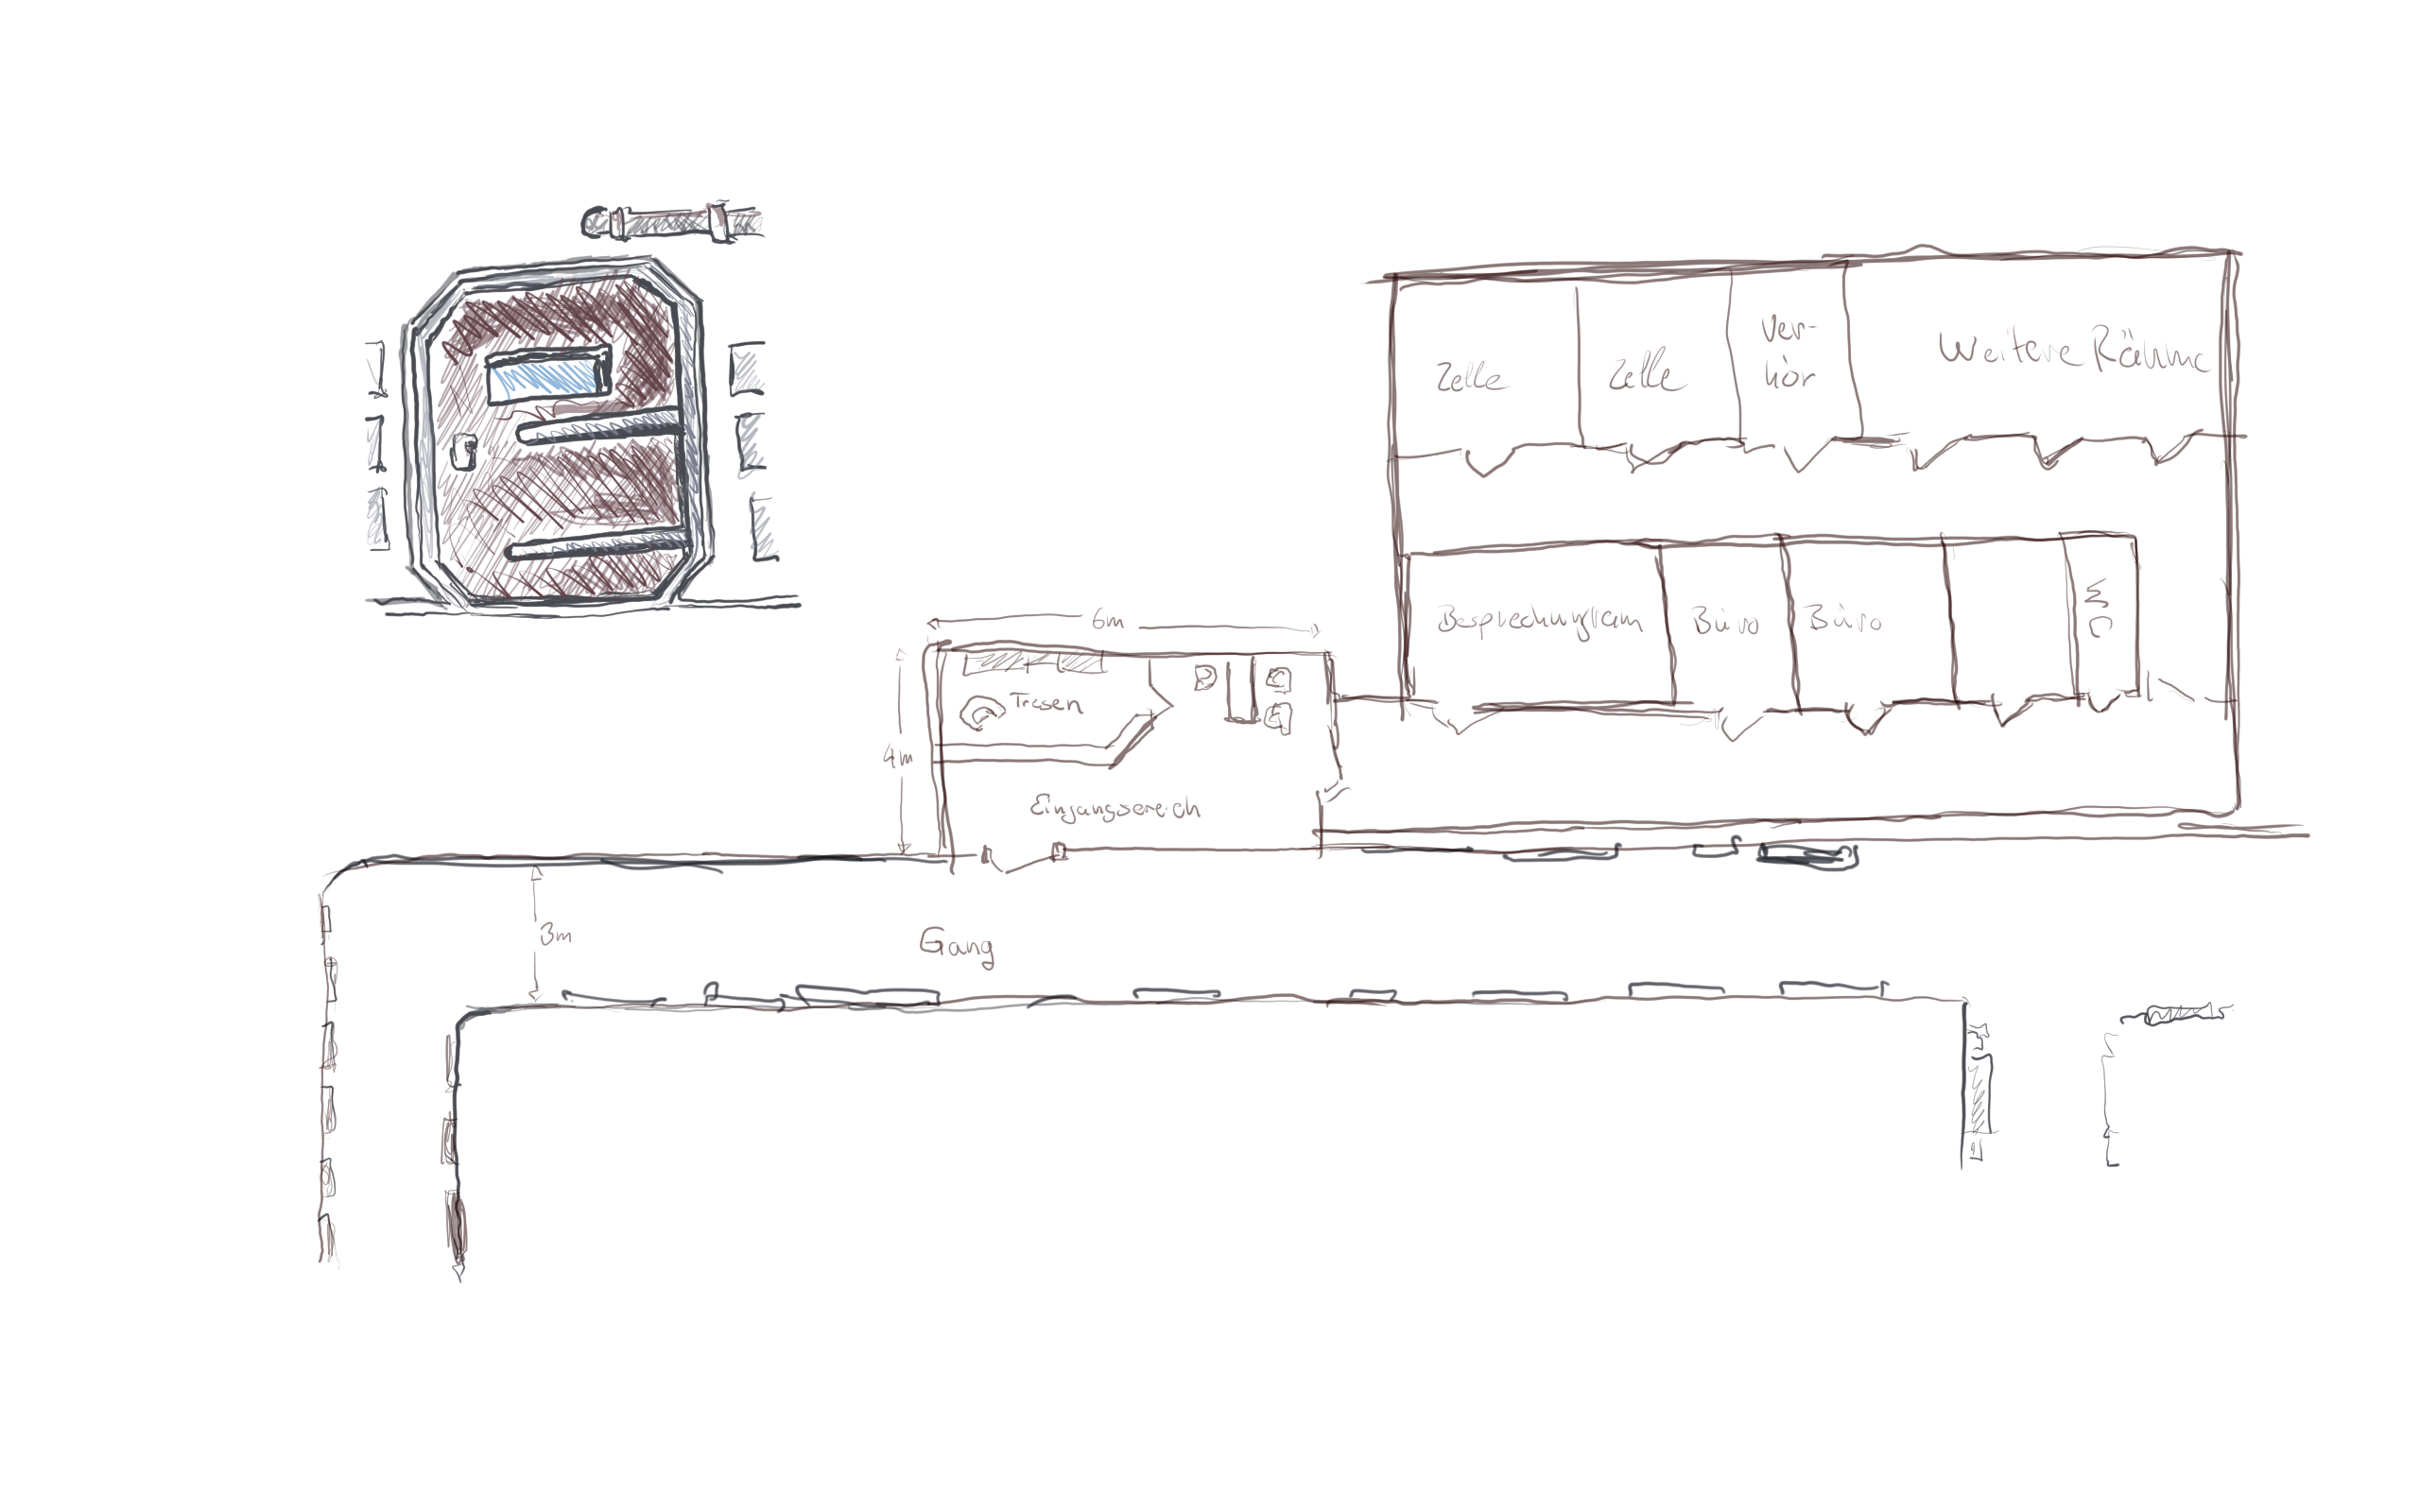
\includegraphics[width=0.9\linewidth]{./images/sicherheitdienst.png}
    \caption{St"utzpunkt Sicherheitsdienst}
\end{figure}

Zuvor: Wenn Henderson und Slingshot den Eingangsbereich des St"utzpunktes unter Kontrolle haben "offnen sie mit der Chipkarte von Karl Sandos oder Luke Lengdon die T"ur zu den hinteren R"aumlichkeiten, den Gef"angniszellen, dem Verh"orraum und anderen B"uros. Die Angreifer sperren die Charaktere und Karl Sandos in eine Zelle zusammen mit den Minenarbeitern und verlassen den St"utzpunkt mit Hanibal, einem der Charaktere und den beiden Frauen der Minenbesatzung als Geisel. Sie hinterlassen im hinteren Teil des St"utzpunkt einen St"orsender, der das ComNetz in der Umgebung des St"utzpunktes ausschalttet, und ein Funkger"at.  

St"urmen die Ermittler den Eingangsbereich des St"utzpunkts k"onnen sie den Eingangsbereich weiter untersuchen. Der Tresen kann mit einer Chipkarte von Grace Anders betreten werden. Hinter dem Tresen sind weitere Blutspuren zu entdecken. N"ahern sie sich der T"ure in die innreren Bereiche oder versuchen die Attent"ster direkt anzusprechen h"oren sie eine Stimme hinter der T"ure die droht die T"ure nicht zu "offnen sonst w"urden Geiseln sterben. Bei dem Sprecher handelt es sich um Slingshot der "uber Sprechfunk solange wie m"oglich versucht den Eindruck zu vermitteln die Entf"uhrer bef"andenden sich im St"utzpunkt. Kurz nachdem die Charaktere den St"utzpunkt betreten haben treffen  weitere Mitarbeiter vom Sicherheitsdienst in Begleitung von zwei Sanit"atern ein. Teil des Eingreiftruppe sind zwei Norms und ein Alpha. Sie tragen die Sicherheitswesten des Sicherheitsdienstes und jeweils einen Bolter. Die Sanit"ater sind Norms. Da es sich bei Hellgate um einen Cynarian St"utzpunkt handelt sind keine Omegas, Streitkr"afte des Protektorats, auf Hellgate verf"ugbar. Angef"uhrt wird der Trupp durch \emph{Luke Dexter} der sich direkt "uber den Verfall in Kenntniss setzen l"asst. W"ahrenddessen l"asst er durch seine Leute unter Unterst"utzung der Ermittler und Grace den Eingangbereich und die G"ange absichern. 

Im Zellentrackt: Im Zellentrackt ist die andere Gruppe von Charakteren zusammen mit den Minenarbeitern eingesprerrt. Es fehlen Personen aus beiden Lagern. Auch ist nicht bekannt wo sich die Entf"uhrer aufhalten. Die Charaktere h"atten jetzt Zeit zu versuchen sich zu befreien oder sich bemerkbar zu machen. Die Zellen sind auf Randalierer und f"ur Aufst"andige gedacht dementsprechend nicht so gut agesichert wie eine Gef"angniszelle. Auch wenn das ComNetz lahmgelegt ist ist die T"ur ist nicht ohne passendes Werkzeug zu knacken.  Ben"otig w"aren ein Magschlossknacker oder Werkzeug zum kurzschlie\3en der Hydraulick. M"oglicherweise k"onnen hier aber Gegenst"ande aus dem Raum oder den 
Taschen der Minenarbeiter zweckendtfremdet werden. Auch ein Lichtschacht w"are eine M"oglichekt zumindest Kontakt nach au\3en aufzunehmen. 
Der Spielleiter sollte je nach Spielflu\3 entscheiden wie viel Zeit an dieser Stelle zur Verf"ugung steht.

Auf der Flucht: W"ahrend der Vorkommnisse im St"utzpunkt sind die Entf"uhrer zusammen mit ihren Geiseln auf dem Weg zu ihrem Shuttle um Valhalla zu verlassen. Kurz nach dem Verlassen des St"utzpunktes haben die Angreifer ihre Kampfausr"ustung gegen schu\3sichere Westen und einfache Bolter getauscht um nicht so leicht aufzufallen. Slingshot, Smith Henderson und Hanibal sind jeweils mit einer Schu\3waffe bewaffnet und treiben die Geiseln vor sich her. Um die PAN Systeme der Geiseln zu st"oren nutzen die Geiselnehmer ein St"orsender mit kurzem Radius.

Verhandlunng mit den Entf"uhrern: Wurde der Eingangsbereich des St"utzpunkts abgesichert k"onnen die Charaktere zusammen mit Luke Dexter in Verhandlung mit den Entf"uhrern treten oder die hinteren R"aume des St"utzpunktes st"urmen. Fordern die Charaktere nach einem Lebenszeichen ihrer Freunde kann Slingshot den entf"uhrten Charakter bitten ein kurzes Wort von sich zu geben bei dem dieser versuchen kann eine Botschaft zu "ubermitteln.

\begin{remarks}
	Die Geiselszene ist auf einen schnellen Szenenwechsel zwischen den Charakteren im St"utzpunkt und den Charakteren die anderweitig Nachforschungen betreiben ausgelegt. Die Szenenwechsel sollten immer so erfolgen dass die \emph{Spieler} nur die wesentlichen Information erhalten die auch ihren Charakteren zur Verf"ugung stehen. D.h.~vor allem mu\3 ein Szenenwechsel erfolgen bevor die Geiselnehmer den St"utzpunkt wieder verlassen damit keiner der Spieler zun"achst erf"ahrt welche weiteren Schritte die Geiselnehmer einleiten.

	Slingshot steht mit Artisan dem Stellvertreter des Protektors und weiterem Attent"ater in Kontakt ohne seine Identit"at zu kennen. Im Auftrag der USI Agenten wird er durch Henderson auf Armageddon eingesammelt und fliegt mit ihm nach Hellgate bevor die Charaktere dort ankommen. Er kann dadurch verfolgen wie Hanibal zusammen mit den anderen Minenarbeitern zum St"utzpunkt der Sicherheitsmannschaft gebracht wird.

	Der erste Angriff sollte so ausgelegt werden, dass die Anreifer die Oberhand behalten aber keiner der Charaktere get"otet wird.
\end{remarks}


\newsection{Showdown auf Hellgate}

Die Entf"uhrer haben ihr Shuttle auf der Au\3enseite von Adrastea bei einer Wartungsschleu\3e nahe dem Raumhafen verankert. Nachdem die Charaktere im St"utzpunkt herausgefunden haben, dass sich die Entf"uhrer nicht mehr dort befinden gibt es mehrere M"oglicheiten die Entf"uhrer aufzusp"uren. Am Erfolgsversprechenden w"are es die nach wie vor auftretenden St"orungen im ComNetz der Station zu verfolgen. F"ur die Navigation im St"utzpunkt m"ussen die Entf"uhrer kurzzeitig den St"orsender deaktivieren. Das gibt den Geiseln die M"oglichkeit eine kurze Nachricht zu "ubermitteln.

Folgende Szenarien die Entf"uhrer zu stellen sind denkbar:

\begin{description}
	\item [Lagerkomplex] Im Lagerkomplex des Raumhafens g"abe es die M"oglichkeit einen Hinterhalt zu legen und die Entf"uhrer zu 		
		"uberraschen.
	\item [Wartungsschleuse] Die Attent"ater und ihre Geiseln haben Hellgate verlassen und dabei ihr Shuttle zu betreten.
	\item [Shuttleverfolgung] Ist das Shuttle bereits gestartet bleibt den Charakteren nur das Shuttle zu verfolgen und zu entern um die 	
		Gefangenen zu befreien.
\end{description}


Wartungsschleuse: Hellgate besitzt neben dem Raumhafen eine Reihe von Ausg"angen die "uber Tunnel an die Oberfl"ache des Mondes ereichbar sind. Sie dienen als Flucht und Rettungstunnel oder geben Zugang zu verschiedenen Sensorplattformen zumeist in Richtung des Jupiters. Das Shuttle der Entf"uhrer hat auf einer Landeplattform mit seinen Andockklammern festgemacht. Der Zugangsbereich zum Landedeck umfasst zwei Luftschleu\3en: Eine als zu- und Ausgang f"ur personen, eine zweite als Eingang f"ur Frachtcontainer. Eine Transportgondel f"ahrt "uber 500m zu einem gro\3en Zwischenlager. Ein Tender"ahnliches Schienenfahrzeug erlaubt es Material von einem angedockten Schiff zur Schleuse zu transportieren. Der Weg zum Landebereich ist "Uberdacht.  Die Schwarkraft auf Adrastea ist vernachl"assigbar. Es herrt mehr oder weniger Schwerelosigkeit. Trotz Magnetstiefeln sollten sich Personen an Handl"aufen einhaken.

Shuttleverfolgung: Die Entf"uhrer versuchen in niedrigem Orbit zu fl"uchten um eine Vorfolgung zu erschweren. In der N"ahe des Jupiters sind Sensoren nur eingeschr"ankt nutzbar. Dies wiederum erlaubt es Angreifern unerkannt von hinten im Schatten des Fusionstriebwerks anzugreifen. Die Geiseln sind im Shuttle im Laderaum eingesprerrt. F"ur ein Enterman"over ist die Dawn of Day am ehesten geeignet. Mit einem Dockingtunnel kann sie an das Shuttle der Entf"uhrer andocken. Die Schleuse in das Schiff kann entweder mit einem Magschlo\3knacker entriegelt oder aufgeschwei\3t werden. Torro Alvarez ist bereit mit seinen Valkyrien den Ermittlern flankenschutz zu bieten und f"ur ein Ablenkungsman"over zu sorgen indem er mit den Etf"uhrern in Verhandlungen tritt. Einer Valkyrie bietet neben einem Piloten auch einer zweiten Person Platz.

Hanibal und Slingshot werden um jeden Preis versuchen ihrer Gefangennahme zu entgehen Der S"oldner hingegen ist nicht bereit bei dieser Mission zu sterben. Den Kampf mit Hanibal und Slingshot sollte

\begin{remarks}
	Bei den drei Optionen ist zu beachten, dass sie in Herausforderung und Zeitaufwand von oben nach unten gestaffelt sind. Zum Zeitpunkt der Entf"uhrung ist der Plot ca.~zu einem Drittel gespielt. Der Spielleiter sollte je nach angepielter Spieldauer sich f"ur eine der Optionen entscheiden.

	Bei der "Uberw"altiging der Entf"uhrer sollte der Spielleiter anpeilen dass sowohl Hanibal als auch Slingshot get"otet oder so stark verletzt werden dass sie nicht mehr verh"ort werden k"onnen. Wurde Hanibal keinem Gehirnscan unterzogen sollte nachfolgend einem Psynchonauten ein Gehirnscan erm"oglicht werden.
\end{remarks}


\newsection{Hellgate Debriefing}

Die Ereignisse auf Hellgate werden von der F"uhrung, Vandermool, Avenger und Blackheart als selhr kritisch gesehen. Alle drei wollen die Erkenntnise geheim halten um zum einen keine Panik auszul"osen und zum anderen den Ermittlern Zeit ver kaufen bevor etwaige weitere Attent"ater aufgeschreckt werden. Desweiteren haben die Ereignisse ein in diesem Ma\3e vorher nicht vorhandenes Mi\3trauen zwischen Cynarian und dem Protektorat geschaffen. Avenger und vor allem Blackheart bef"urchten eine verdeckte Operation der Cynarian Corporation. Vandermool ist beunrufigt, dass die Geschehnisse genau so eine Reaktion ausl"osen.

Kurz nach dem Sieg "uber die Entf"uhrer laden Vandermool, Avenger und Blackheart die Ermittler zu einem geheimen virtuellen Treffen in einem hermetisch abgeschrimten Raum der Valhalla Station ein. Die Ermittler k"onnen nochmal in allen Details "uber die Geschehnisse berichten. Die weitern Nachforschungen m"ussen unter strengster Geheimhaltung forgesetzt werden. Die Erkenntnisse der Gehirnmanipulation deuten auf manipulierte Cybernetischen Modulen hin die auf Kallisto eigesetzt wurden. Aus diesem Grund werden die Charaktere gebeten dort ihre Nachforschungen fort zu f"uhren.

Veranlasst durch Vandermool werden die Leichen oder verletzten Attent"ater umgehend auf die Nike Station transportiert um dort n"aher untersucht werden zu k"onnen. Blackheart setzt durch das Mitglieder der Mutantennation den Untersuchungen beiwohnen.

\begin{remarks}
	Das Briefing auf Hellgate ist die erste Gelegenheit im Plot bei der Vandermool, Avenger und Blackheart zusammen auftreten. Der Spielleiter sollte in diesem Gespr"ach zum einen das dominante Auftreten Vandermools und das Mi\3trauen von Blackheart gegen"uber Vandermool vermitteln.

	Um die mehreren Milionen Kilometer zwischen den einzelnen Orten der Mission zu vermitteln sollte der Spielleiter die "Ubertragungszeit von mehreren Sekunden in die Dialoge einstreuen.

	Der Treffen dient im wesentlichen dazu die Spieler in Richtung Valhalla zu orientieren und die Nachhorschungen auf Valhalla zu beenden.
\end{remarks}

\newsection{Im Zentrum von Valhalla}

Der Anflug auf Valhalla bringt die Ermittler gleich zum Zentrum der Stadt, dem Raumhafen. Im Orbit "uber Valhalla halten sich gro\3e Frachter in Position. Shuttles und F"ahren verkehren zwischen Kallisto den gro\3en Schiffen und anderen Zielorten im jovianischen System. Bei der Ankunft im Raumhafen hundert Meter unterhalb der eisigen Oberfl"ache des Mondes herrscht entsprechend reges Treiben. Der Dawn of Day wird routiniert eine Andockbucht zugewiesen. Mit gro\3en Formalien m"ussen die Ermittler nicht rechnen. Sie sind bereits angek"undigt. F"ur Walhalla wie auch f"ur nahezu alle Siedlungen und Stationen im Sonnensystem ist ein k"unstlicher Tag und Nachtzyklus durch passende Lichverh"altnisse Lebensrhytmen eingerichtet. F"ur den Raumhafen gilt so ein Zyklus nicht. Im Raumhafen herrscht Tag und Nacht Hochbetrieb. 

%\bottomimage{images/armytank.png}

\newsection{Auf dem Garnisonsst"utzpunkt}

Ein erster Anlaufpunkt der Charaktere w"are vermutlich der Garnisonsst"utzpunkt des Protektorats. Der Oberbehehlshaber des St"utzpunktes ist der Omega \emph{Commander Lockhead} der bereits "uber das Eintreffen der Ermittler informiert ist. Nach der Aufkl"arung des Frachterungl"ucks auf Armageddon hat er die Cowboybrigade inhaftieren lassen und h"alt sie seit dem in Untersuchungshaft. Der Commander ist "uber die Vorg"ange auf Hellgate informiert und bietet diesbez"uglich den Ermittlern seine Hilfe an. Er kann den Ermittlern f"ur Untersuchungen im Umfeld vom Raumhafen, der Garnison, dem Headquarter und Rosenfurth seinen Adjuntanten \emph{Firedon} zur Verf"ugung stellen. Zu Fragen nach der Cowboybrigade kann Lockhead erl"autern, dass als Vorbereitung f"ur den Einsatz der neuen Drohnen und anderer technischer Ger"ate die auf Armageddon zum Einsatz kamen die ganze Cowboybrigade mit neuen Talentchips vor 1,5 Monaten in der Klinik \emph{Rondra Hospital} ausgestattet wurden. Die Kosten hat die Garnison "ubernommen. Die Cowboybrigade ist seit vier Monaten am Raumhafen f"ur Wartungsarbeiten an Schiffen und Ger"atschaften der Garnison besch"aftigt. Auch nach ihrer Versetzung zur Garnison ist Sonja Frost ihre personelle Vorgesetzte.

\begin{remarks}
	Gewonnene Informationen: Kontakt Firedon. Cowboybrigade seit vier Monaten bei der Garnison im Raumhafen t"atig. Vor 1,5 Monaten einsetzen von Talentchips in der Rondra Klinik. Kontakt Sonja Frost.
\end{remarks}



\newsection{Voruntersuchung zur Cowboybrigade}

Gehen die Charaktere davon aus das weitere Mitglieder der Cowboybrigade ebenfalls eine Gehirnmanipulation unterzogen wurden k"onnen sie Firedon veranlassen einen der vier in einer Klinik, Rondra Hospital oder die Alexandr Klinik untersuchen lassen. Das Rondra Hospital f"uhrt als gr"o\3tes Hospital in Valhalla alle medizinischen Eingriffe f"ur den Garnisonsst"utzpunkt durch. Vertrauen die Charaktere dem Rondra Hospital nicht schl"agt Firedon die \emph{Alexandr Clinic} vor. Der leitende Arzt Dr.~Spinner zeigt sich zwar erstaunt warum man sich an seine Klinik und nicht an das Rondra Hospital wendet ist aber bereit eine Untersuchung durchzuf"uhren. Bei den nicht invasiven Untersuchungen durch eine Klinik lassen sich keine Manipulationen feststellen. Die verbauten technischen Einheiten wirken unauff"allig. Wenn die Charaktere allerdings noch keine n"aheren Informationen von Nike erhalten haben ist auch nicht klar auf was der Arzt achten sollte. Selbst mit weiteren Informationen werden bei der Untersuchung keine Auff"alligkeiten festgestellt. Der Rest der Cowboybrigade ist ebenfalls sauber.

\begin{remarks}
	Gewonnene Informationen: Ein Gehirnscan zeigt keine Anomalien.
\end{remarks}


\newsection[Nachforschungen im Rondra Hospital]{Nachforschungen im Rondra\newline{}Hospital}

Bez"uglich Rondra Hospital k"onnte der Verdacht aufkommen, dass dort die Manipulationen an den Gehirnen von Hanibal und Slingshot durchgef"uhrt wurden. Auf drengen von Commander Lockhead w"are ein Termin mit dem Klinikleiter \emph{Prof.~Dr.~Henry Sanders} m"oglich. Der Klinikleiter empf"angt die Charaktere in einem ger"aumigen B"uro. Sanders ist ein Norm im Alter von "uber 50 Jahren mit gepflegtem Aussehen, grau milierten Haaren. Bei Fragen zur Cowboybrigade verweist er die Charaketere an Brenda Ben die er auch gleich bittet die Ermittler zu empfangen. Brenda Ben ist eine symphatische und erfahrene "Arztin, Mitglied des Leitungsteams der Praxis. Routiniert kann sie von Ben Reuthers Unterlagen anfordern und an behandelnden "Arzte und Physiotherapeuten verweisen. Sie selbst hat allerdings nur begrenzt Zeit und wird bald auch zu einer Operation gerufen. Die Inforationen aus der Klinik entsprechen den von Informationen Commander Lockhead.

\begin{remarks}
	Gewonnene Informationen: Kontakte Prof.~Dr.~Henry Sanders, Brenda Ben. Keine ungew"ohnlichen Vorkommnisse.
\end{remarks}


\newsection{R"uckmeldung von Nike}

Zwei Tage nach Ankunft werden die Ermittler von Dr.~\pinyin{Wang2} \pinyin{Chen2} kontaktiert. Er f"uhrte die Untersuchungen an dem immer noch bewustlosen Slingshot und an Hanibal auf der Nike Station durch. \pinyin{Wang2} \pinyin{Chen2} konnte in dem Gehirn von Hanibal inaktive Nanobots entdecken. Die Nanobots haben sich "ahnlich dem Comandmodule mit den Synapsen des Gehirns verbunden. Im Gehirn von Slingshot sind elektrische Impulse die nicht dem Gehirn selbst oder dem Commandmodul zuordenbar sind gemessen worden. Die genaue Funktion der Nanobots konnte noch nicht festgestellt werden. Es mu\3 aber von einem hoch komplexen verteilten System ausgegangen werden.

\begin{remarks}
	Gewonnene Informationen: Die Bewustseinsver"anderung der Attent"ater wurde durch Nanonbots im Gehirn ausgel"ost.
\end{remarks}


\newsection{Sonja Frost}

Eine weitere Anlaufstelle im Zentrum von Hellgate ist \emph{Sonja Frost}. Sie ist der Chief Officer des Hangar Decks des Raumhafens. Sonja Frost ist dementsprechend schwer zu erreichen. Ein Anruf durch den St"utzpunkt ist notwendig um "uberhaupt einen Termin zu vereinbaren. Sonja ist in ihrem B"uro neben dem Hangar anzutreffen. Das B"uro ist mit technischen Ger"aten, Holoprojektoren und Tafeln vollgestellt. Es herrscht ein reges Ein- und Ausgehen und Sonja verteilt durchgehend Anweisungen. Von Sonja erfahren die Ermittler, dass die Cowboybrigade vor ca.~1,5 Jahren vom G"urtel in das Jovianischen System gewechselt hat und dort am Raumhafen untergekommen ist. Vor vier Monaten wurden sie dann an das Milit"ar "uberwiesen. Der medizische Eingriff bei der Cowboybrigade wurde in Abstimmung von Commander Lockhead und ihr vor 1,5 Monaten veranlasst und erwartungsgem"a\3 durchgef"uhrt und bezahlt. Sonja Frost berichtet, dass die Mitglieder der Cowboybrigade, als sie unter dem Pseudonym "`die glorreichen F"unf"' am Raumhafen besch"aftigt waren. Aufgrund ihrer heiteren, skurrielen Art aber auch wegen ihrer Zuverl"assigkeit sind sie im Hangar Decks bekannt und wertgesch"atzt.  Den Spitznamen Cowboybrigade erhielten sie erst bei der Besch"aftigung in der Garnison als sie begannen gegen"uber Stetson zu salutieren. Nach dem Einsetzen der Talentchips im Rondra Hospital kehrten die f"unf nach 2 Wochen wieder zum Dienst zur"uck. Slingshot allerdings meldete sich ein paar Tage sp"ater krank und kehrte erst drei Wochen, kurz vor der "Uberstellung nach Armageddon zur"uck. N"aheres kann sie dazu auch nicht sagen. Bevor die Charaktere das B"uro verlassen f"allt ihr noch ein, dass sich gestern zwei Herren in Anz"ugen nach den Ank"ommlingen mit der Down of Day erkundigt haben. Einer der beiden war gro\3, mit einer T"ursteher Statur, sehr gepflegt mit einem blonden B"urstenschnitt. Der andere war unauff"allig und hatte nicht gesprochen. Informationen "uber die Ermittler konnten den beiden nicht gegeben werden (O--Ton "`k"onnte ja jeder kommmen"'). Aufzeichnungen von den beiden sind ihr nicht bekannt.


\begin{remarks}
	Gewonnene Informationen: Cowboybrigade alias "`die glorreichen F"unf"' seit 1,5 Jahren im jovianischen System, t"atig am Raumhafen. Vor 4 Monaten Wechsel zur Garnison. Vor 1,5 Monaten Einsetzen des Talenzchips. Slingshot krank gemeldet f"ur drei Wochen. Zwei Anzugtr"ager haben sich nach der Dawn of Day erkundigt.

	Bei den beiden die sich nach dem Schiff der Ermittler erkundigt haben handelt es sich um Smith--Singer und Frederic Johnson was allerdings nicht "uber den Raumhafen in Erfahrung zu bringen ist.
\end{remarks}


\newsection{Die Cowboybrigade im Verh"or}

Die Ermittler k"onnen Firedon beauftragen die inhaftierte Cowboybrigade in einem Verh"orraum vorzuf"uhren. Stetson fl"atscht beim eintreten der Charaktere im Sitz mit einem Zahnstocher im Mund und einem verbeulten Stetson auf dem Kopf. Beim "offnen der T"ur r"uckt er alarmiert aufrecht auf seinem Stuhl zurecht. Quicksilver Rod mischt nerv"os aber virtuos ein Deck Spielkarten. Joe Rider sitzt finster blickend eingesunken auf seinem Stuhl. Tom Gunslinger wendet den Blick erwartungsvoll in Richtung der Eintretenden. Werden die F"unf zusammen befragt wendet sich Stetson als erster an die Charaktere und fragt was ihnen vorgeworfen wird, was mit Slingshot los ist und wann sie wieder entlassen werden. Der Gruppe wurde offensichtlich keine n"aheren Informationen zu den Geschehnissen auf Hellgate gegeben. Stetson und Tom Gunslinger geben bereitwillig Auskunft und beteuern, dass die Gruppe sich nichts zu schulden kommen hat lassen. Sie gehen nach wie vor davon aus das es sich auf Armageddon um einen Unfall gehandelt hat. Quicksilver Rod blickt bei einer Befragung immer wieder zu Stetson. Seine Finger scheinen dabei ein Eigenleben zu f"uhren und einen Kartentrick nach dem anderen zu vollf"uhren ohne das Rod Notiz davon nimmt. Bei Joe Rider vergeht nach jeder Frage erst fast eine Minute bevor er antwortet. Die Antworten beschr"anken sich nur auf das Gefragte und enthalten nicht ein unn"otiges Wort. Auf eine psychnoatische Untersuchung reagiert die Gruppe leicht panisch keiner eine Ahnung hat was auf sie zukommt. Die Untersuchung lassen sie aber "uber sich ohne Gegenwehr ergehen. Die Untersuchung best"atigt dass ihre Gehirne sauber sind. Angesprochen auf die Eingriffe in der Rondra Klinik schildern sie, dass sie in der Klinik neue Talentchips mit anschlie\3endem Training erhalten haben. Eine Frage ob es bei Slingshot Komplikatioen gegeben hatte wird vewrneint. Allerdings erfahren die Ermittler dass Slingshot im Gegensatz zu den anderen kein ausgebildeter Shuttle-- und Drohnenpilot ist sondern nur ein hervorragender Schiffstechniker. Slingshot hatte immer davon getr"aumt auch eine Flugausbildung zu erhalten. Offensichtlich hat er sich nach dem Aufenthalt im Rondra Hospital deshalb selbst auf die Suche nach einer passenden Riggersteuerung gemacht. Offensichtlich wurde er kurz vor der Versetzung nach Armageddon f"undig. Er hatte sich nach dem Aufeinthalt in der Rondra Klinik wie es aussieht eine Riggerstuerung einbauen lassen. Wie er die daf"ur entstehenden Kosten aufbringen konnte wollte er den anderen nicht verraten. Ebenso wenig wo er den Eingriff hat durchf"uhren lassen und wo er sich danach aufgehalten hat. Ein paar Tage nach der Entlassung aus dem Rondra Hospital hatte er angefangen die Freizeit oft alleine zu verbringen. "Uber den Barmann und Besitzer des Batcave konnten seine Freunde in Erfahrung bringen, dass er wohl eine h"ubsche Frau kennen gelernt hatte. Darauf anesprochen tat er allerdings immer betont geheimnissvoll. Weitere Informationen sind von der Cowboybrigade  nicht in Erfahrung zu bringen.

\begin{remarks}
	Gewonnene Informationen: Slingshot hat sich eine Riggersteuerung implantieren lassen. Finanzierung unklar. Geheimnisvolle Freundin. 
	
	Es handelt sich hierbei um Carina alias Fleur Soleil was der Cowboybrigade und dem Barmann im Batcave allerdings nicht bekannt ist.
\end{remarks}

\newsection{Zwischenfall auf Fenris (optional)}

Der Zwischenfall auf Fenris kann z.B. genutzt werden wenn die Charaktere auf Hellgate nicht mit den KIs in den K"opfen der beiden Attent"ater in Kontakt kommen konnten. Der Vorfall hilft auch ein agressiveren Vorgehen von Blackheart im sp"ateren Spielverlauf authentischer zu machen. Er ist eine gute M"oglichkeit die kosmonautischen F"ahigkeiten der Charaktere zum Einsatz zu bringen. Der Zwischenfall auf der anbdren Seite verl"angert allerdings auch den Spielablauf signifikant ohne zwingende Relevanz f"ur die Geschichte zu haben. Er ist deshalb als optional gekenntzeichnet.

Kurz nach den ersten Ergebnissen der Nachforschungen auf Kallisto werden die Charaktere vom Komandanten Lord Commander Bolder der Fenris Station kontaktiert. Auf der Raumbasis konnte ein Attent"ater dingfest gemacht werden, der die Computersysteme der Station zu manipulieren versuchte. Beim Attent"ater handelt es sich um den Omega Commander Tiger. Commander Tiger beteuert angeblich, von dem Attentat nichts zu wissen, obwohl er sich seiner Festnahme widersetzte und einen Kameraden lebensgef"ahrlich verletzte. Die Ermittler werden gebeten, sich schnellstm"oglich auf der Fenris Station einzufinden, um dem Verh"or beizuwohnen.

Beim Landeanflug auf die Fenris Station kommt es zu einem unerwarteten Zwischenfall. Die Verteidigungsanlagen der Station nehmen das Shuttle der Ermittler mit Gau\3kanonen kurzzeitig unter Beschuss. Dabei wird das Eind"ammungsfeld des Fusionstriebwerks stark besch"adigt, und es kommt zu einem Druckverlust im Schiff. Weiter kommt es zu einem Ausfall des Zentralcomputers. Wird das Shuttle nicht von einem der Ermittler gesteuert, kommt der Pilot ums Leben.

Was genau passiert ist, erfahren die Shuttleinsassen zu diesem Zeitpunkt nicht. Das Schiff wird ordentlich durchgesch"uttelt, und die Passagiere werden unsanft aus der virtuellen Realit"at des Bordsystems gerissen. Notbeleuchtung und der Schiffsalarm wei\3en unmissverst"andlich auf den Ernst der Lage hin. Alle Passagiere tragen gl"ucklicherweise einen Druckanzug, um die Kr"afte bei Abflug und Anflug zu kompensieren, m"ussen aber noch die Atemmaske anlegen, die jeweils in einem Fach der Beschleunigungsliege bereit liegt. Um eine Explosion des Fusionstriebwerks zu verhindern, muss als erstes der Zentralcomputer neu gestartet und dann eine Notabschaltung ausgel"ost werden. Nach dem Abschalten des Fusionstriebwerks tritt im Shuttle sofort Schwerelosigkeit ein.

Bei einem Abstand von rund 1200 km rast das Shuttle nun mit 500 m/s auf die Fenris Station zu. Der Bordcomputer l"ost Kollisionsalarm aus. Mittels Man"ovrierd"usen k"onnte die Flugbahn korrigiert werden, um an Station vorbei zu fliegen, doch die Man"oversteuerung kann die D"usen nicht ausrichten. D.h.~nur durch einen Au\3neinsatz kann die D"use in Position gebracht werden.

W"ahrend ein oder zwei Ermittler die D"use manuell ausrichten, kann einer der Ermittler, die Funkanlage die ebenfalls ausgefallen ist, wieder in Betrieb nehmen. Die Anlage muss auf die Notantenne umgeschalten werden, da die Hauptantenne beim Angriff besch"adigt wurde. Ist die Funkanlage wieder verf"ugbar, kann ein Notruf abgesetzt werden, der von der Flugleitung der Fenris Station beantwortet wird. Mit geknickter Stimme fragt der Flugleitstand nach der Situation auf der Dawn of Day und meldet, dass die Verteidigung der Station aufgrund einer noch nicht gekl"arten Fehlfunktion das Shuttle unter Beschuss genommen hat. Die Station entsendet daraufhin ein Rettungsshuttle, um die Dawn of Day zur Fenris-Anlage zu schleppen.

Lord Commander Bolder in Begleitung von zwei weiteren Omega-Soldaten nimmt die Ermittler pers"onlich in Empfang. Er erkl"art den Besuchern, dass vermutet wird, dass der Angriff auf das Shuttle mit dem Sabotageakt in Zusamenhang steht. Die Verteidigungsanlage ist derzeit komplett deaktiviert, heruntergefahren und vom Rest der Stationssysteme getrennt. Leider m"ussen Computerspezialisten, die dem Problem Herr werden k"onnen, erst angefordert und eingeflogen werden. Lord Marshall Blackheart ist bereits "uber die Vorkommnisse auf der Station informiert und hat angek"undigt, sich selbst ein Bild vor Ort machen zu wollen.

Laut Commander Bolder wurde Tiger "uberrascht, w"ahrend er sich im zentralen Computerkabinett an den Speicherb"anken zu schaffen machte. Als nicht Techniker h"atte er zu diesem Bereich keinen Zugriff gehabt und sollte eigentlich auch  keine Expertise f"ur die Rechenanlage besitzen. Bei seiner Entdeckung griff er sofort zu seiner Elektropistole und feuerte mehrere Sch"usse auf den Sergeant der Patrouille ab, die ihn entdeckt hatte. Der Sergeant ging zu Boden. Sein Begleiter konnte Tiger allerdings "uberw"altigen und Hilfe anfordern. Bei der Erstbefragung beteuerte der Gefangene, sich in keinster Weise an die Vorg"ange erinnern zu k"onnen.

Commander Tiger ist in einer Arrestzelle zum Verh"or festgesetzt worden und wird dort von zwei Soldaten bewacht. Der Gefangene sitzt in einem durch Gitter abgesperrten Teil der Zelle. Im Besucherteil halten zwei bewaffnete Omega Wache. Der Attent"ater wirkt beim Eintreffen der Ermittler stark angespannt, bei\3t die Z"ahne zusammen und antwortet auf keine Fragen. Lord Commander Bolder erw"agt, Tiger durch Wahrheitsdrogen gespr"achig zu machen, will daf"ur aber erst die Ankunft von Blackheart abwarten. Bestehen die Ermittler darauf, einen Gehirnscan durchf"uhren zu wollen, wird ihnen diese Bitte widerwillig gew"ahrt. Der Psychonaut des Teams muss daf"ur den abgesperrten Teil der Zelle betreten. Commander Tiger ist mit Hand- und Fu\3fesseln auf einem Stuhl fixiert. Betritt der Psychonaut den Gefangenenteil, wird Tiger pl"otzlich vollkommen ruhig und bekommt einen glasigen Blick. Kurz darauf l"osen sich die elektronisch verriegelten Fesseln, und er st"urzt sich auf den Ermittler. Die Wachen ziehen beide ihre vollautomatischen Railgun-Pistolen und w"urden den Gefangenen niederschie\3en sofern niemand eingreift und sie freies Schu\3feld bekommen.

Kann der Gefangene lebendig "uberwunden werden, so kann der Psychonaut zur Tat schreiten. In den Erinnerungen des Commanders findet der Psychonaut seltsam artifiziell wirkende Gedankeng"ange mit Matrizen aus Entscheidungsb"aumen. Nach diesen Erkenntnissen wird der Psychonaut mental durch Tigers KI angegriffen. Ein "Uberwinden der KI f"uhrt unweigerlich zum Gehirntot des Commanders. Den letzten Gedanken, den der Psychonaut aufschnappt, ist "`Befreit uns"'.

Wollen die Ermittler auch die Fehlfunktionen im Computersystem untersuchen wird das einige Stunden in Anspruch nehmen. Im Computersystem finden sich eindeutige Spuren einer k"unstlichen Intelligenz, die ebenfalls etwaige Analysten angreift.

W"ahrend sich die Ermittler dem Computersystem widmen, trifft Lord Marshall Blackheart auf der Station ein und l"asst sich im Beisein der Ermittler des Protektorats "uber den Stand der Ermittlungen informieren. Die Cynarian Ermittler werden dabei ausgeschlossen (milit"arische Angelegenheiten).

\begin{remarks}
	Das Gedankenduell kann als Matrixkampf ausgefochten werden.
\end{remarks}

\newsection{Treffen mit Smith-Singer (optional)}

W"ahrend die Ermittler den ersten Hinweisen auf Valhalla nachgehen erh"alt einer der Charaktere, vorzugsweise ein Alpha aber kein Omega eine Nachricht von einem Herrn Smith--Singer bzgl.~einem Informationsaustausch zu den Vorg"angen auf Hellgate. Der Nachrichtensender gibt sich als Beobachter im Auftrag des Transnationalen Konzernrates aus. Bei einer R"uckfragen bei Cynarian oder dem Protektorat werden die Ermittler gebeten den Termin wahr zu nehmen aber keine relevanten Informationen preis zu geben. Ob Smith--Singer wirklich im Auftrag des Konzernrates t"atig ist l"asst sich nicht klar bestimmen ist aber auch nicht auszuschlie\3en. Die Ermittler sollen in Erfahrung bringen was sein Auftrag ist und "uber welche Informationen er verf"ugt. Smith--Singer schl"agt vor im Stadtteil Rosenfurth einen Kaffee trinken zu gehen. Er w"urde sich dabei gerne allein mit dem Ermittler treffen.

Kommt der Ermittler alleine wird er Smith--Singer im "`Au\3enbereich"' des Kaffees nahe dem Eingang antreffen. Smith--Singer ist hoch gewachsen und hat eine athletische kr"aftige Statur. Die Finger sind manik"urt, das L"acheln makellos. Smith--Singer hat einen B"urstenhaarschnitt mit wei\3blonden Haren. Er tr"agt einen teueren ma\3geschneiderten Anzug. Die holograhisches Visitenkarte mit authentischem Konzernrats Logo weist ihn als Mitarbeiter des Konzernrates aus. Smith--Singer erkl"art, dass er als Beobachter im Auftrag des Konzernrates in das Jovianische System entsand wurde um den Aufbau der HE-3 Produktion mitzuverfolgen und eine f"ahre Zusammenarbeit der hiesigen Konzerne sicherzustellen. In diesem Zuge sind ihm die Attentate und die beunruhigende Erkenntniss einer Manipulation der Attent"ater zu Ohren bekommen. Wer seine Informationsquelle ist gibt Smith--Singer nicht an. Er fragt den Protektoratsermittler nach seiner Einsch"atzung der Bedeutung, dass die Attent"ater aus den Reihen der Mutanten gew"ahlt wurde und wen man als Drahtzieher hinter den Attentaten vermutet. Wenn das Gespr"ach anf"angt abzuebben wird er sich freundlich verabschieden begleicht die Rechnung, w"unscht noch einen guten Tag und verschwindet in der Menge.

Mit dem Treffen legt Smith--Singer die Grundlage f"ur ein Eingreifen des Konzernrates mit der USI als Drahtzieher. Zudem schafft er sich selbst mehr Handlungsspielraum indem er sich als Mitarbeiter des Konzernrates platziert. Desweiteren ist er auch daran interessiert sie Ermittler pers"onlich kennen zu lernen um sie besser einsch"atzen zu k"onnen.

\begin{remarks}
	Gewonnene Informationen: Bekanntschaft mit Smith--Singer.	
\end{remarks}

\newsection{Batcave}

Das Batcave ist die Stammkneipe der Cowboybrigade. Der Wirt Lenny Kilkenny auf die Cowboybrigade angesprochen best"atigt das sie regelm"a\3ige G"aste in seinem Pub waren aber wohl nach Armageddon versetzt wurden. Angesprochen auf Slingshot und seine Freundin best"atigt er, dass Slingshot vor vielleicht drei Wochen ein oder zwei mal mit einer h"ubschen Norm im Batcave zu Besuch war. Sie hatten sich immer an einen hinten gelegenen Platz gesetzt. Slingshot hat dabei immer die Gatr"anke an der Theke geholt wodurch Kilkenny keine Gelegenheit hatte mit der Frau pers"onlich zu sprechen. Aufgefallen sind ihm ein schwarzes samtiges Kleid mit Kapuze und nat"urlich die langen und kunstvollen rot schirmenden Haare. Weiteres kann er zu der Besucherin nicht beisteuern.

Neben den Informationen zur Cowboybrigade kann Lenny Kilkenny die Charaktere an G"aste und Bekannte verweisen die mehr Auskunft "uber den Verkauf von Cyberware au\3erhab der offiziellen Wege geben k"onnen.

\begin{remarks}
	Gewonnene Informationen: Freundin mit auff"alligen rot leuchtenden Haare. 
	
	Bei der Freundin handelt es sich um Carina alias Fleur Soleil was die Charaktere allerdings nicht in Erfahrung bringen k"onnen.
\end{remarks}	

\newsection{Kliniken und Konzerne auf Kallisto}

Anlaufstellen f"ur weitere Ermittlungen k"onnen lokale Niderlassungen von Produktionsfirmen und H"andlern wie auch Kliniken sein, die Cyberware implantieren.

Alle Kliniken, die auf Kallisto inoffizielle Implantate verbauen, befinden sich in Valhalla au\3erhalb \emph{Headquarter}, \emph{Rosenfurth} und dem Raumhafen. Bei den Nachforschungen au\3erhalb \emph{Headquarter}, \emph{Rosenfurth} und dem Raumhafen werden die Soldaten aus der Garnison die Ermittler nicht weiter begleiten. An den R"ander von \emph{Paradise City} und \emph{Neu Gr"oning} endet der Einflu\3bereich des Protektorats und man will Spannungen vermeiden. Auf Nachfrage k"onnen die Ermittler erfahren das "uber einen gro\3en Teil Valhalla verschiedene Band unter der Schirmherschaft des Luna--Syndikats herrschen. Au\3erhalb des Headquarters, Rosenfurth und dem Raumhafen ist die Anbindung an das ComNetz nur sp"arlich. Die Charaktere k"onnen ein Sprechfunkger"at an die Hand bekommen wenn sie danach fragen um den St"utzpunkt im Zweifel erreichen zu k"onnen. Das Sprechfunkger"at hat aber auch nicht "uberall Empfang wodurch die Gruppe oft auf sich allen gestellt ist.

Die Kliniken in Valhalla m"ussen einzeln besucht werden. Ein zentrales Verzeichnis der Kliniken besteht nicht. Es m"ussen vor Ort in den jeweiligen Sektoren der Stadt Erkundigungen in Nachtclubs und Lokalen eingezogen werden. Ein erster Anlaufpunkt k"onnte der Schieber \emph{Henk Brothers} sein an den Lenny Kilkenny, der Barmann des Bat Cave sie verwei\3en kann. Henk Brother verweilt "ublicherweise im \emph{Green Mile}, einem der bessren Lokale am Rande von Paradise City zu Rosenfurth. Ein nicht unerheblicher Teil der Wirschaft auf Valhalla au\3erhalb der zentralen Bezirke um den Raumhafen wird vom Luna--Syndikat kontrolliert. Das gilt dementsprechend auch f"ur Schieber, Stra\3endocs und "Arzte mit Nebenberuf. "Arzte werden zu inoffiziellen Behandlungen ohne Genehmigung des Luna--Syndikats bestenfalls ausweichende oder schwammige Ausk"nfte geben. Das gleiche gilt f"ur Schieber oder sonstige Personen die von den Ermittlern bez"uglich medizinischer Eingriffe oder Bodyware befragt wewrden. Bei eigenen Nachforschungen werden die Charaktere keine neuen Erkenntnise gewinnen. Slingshot oder die Cowboybrigade ist in den Etabilments die von den Charakeren besucht ebenfalls  nicht bekannt. In Bezug auf eine Frau mit auff"alligen langen roten Haaren erf"ahrt man von einigen T"anzerin mit langen braunen Haaren und von einer S"angerin mit auff"alligen aber blonden Haaren.

Die lokalen Firmen im Headquarter die im Bereich Cyberware Technologien und Dienstleistungen anbieten (siehe Anhang) geben Informationen zu ihren Produkten bereitwillig heraus weigewrn sich aber Informationen "uber Kunden oder Lieferwege sowie Informationen zu ihren Mitarbeitern heraus zu geben. Den Konzernen steht als Konsulat f"ur Rechtsfragen eine kleine Niederlassung des Konzernrates zur Verf"ugung. Der Status der Niederlassung entspricht in etwa der einer Botschaft. Auf die R"uckfragen ob Smith--Singer f"ur den Konzernrat arbeitet wird mit der R"uckfrage geantwortet in welcher Angelegenheit man mit ihm gerne sprechen w"urde. Es wird das Angebot unterbreitet eine Nachricht zu hinterlassen. Auch Cynarian hat in diesem Zusammenhang keine besseren M"oglichkeiten.

\begin{remarks}
	Um die unfruchtbaren Nachforschungen der Ermittler nicht zu sehr in die L"ange zu ziehen sollte der Spielleiter den Eindruck einer Wand des Schweigens zu vermittlen. Wie oben Beschrieben sollte den Spielern z.B.~bei R"uckfrage auf dem Milit"arst"utzpunkt vermittelt werden, dass wahrscheinlich das Syndikat ihnen hier die Kn"uppel zwischen die F"u\3e wird.

	Durch die "ubernahme der HE-3 Produktion im jovianischen System durch Cynarian hat die USI ihre Vormachtstellung in diesem Gebiet verloren und das Feld weitestgehend ger"aumt. Aus diesem Grund besitzt die USI keine offiziellen Niederlassungen mehr rund um den Jupiter. Das Konsulat des Konzernrates allerdings wurde vor der Aufgabe des Systems von der USI finanziert und gef"uhrt und ist ensprechend mit dem Konzern vernetzt, bietet dadurch auch den USI Agenten die Tarnidentit"at als Konzernratsmitarbeiter.

	Eine Ablehnende Haltung der Konzerne wird von Blackheart als weiteren Anlassgrund genommen Ma\3nahmen gegen Valhalla zu unternehmen.
\end{remarks}

\newsection[Zusammestross mit dem Luna-Syndikat]{Zusammestross mit dem\newline{}Luna-Syndikat}
\newcommand{\xl}{\pinyin{Xiao3} \pinyin{Long2}}
\newcommand{\xlsn}{\pinyin{Xiao3} \pinyin{Long2}}

Das Luna--Syndikat verfolgt die Ermittler seit dem Verlassen des Raumhafens und Rosenfurth genau. Durch einen W"urfelwurf auf Investigation bemerken Charaktere dass die Gruppe immer wieder verfolgt wird. Die Verfolger scheinen immer wieder unterschiedliche Personen zu sein, Ghetto Kids, Schl"ager, d.h.~zwielichte Personen die verschwinden wenn sie das Gef"uhl haben entdeckt worden zu sein. Nachdem sich die ersten Nachforschungen als nicht erfolgreich erweisen k"onnte die Gruppe beharrlich weiter suchen, einen Verfolger aufgreifen, einen der Schieber oder "Arzte in die Mangel nehmen oder den Kontakt zum Syndikat suchen. 

Unabh"abngig davon f"ur welche Option sich die Spieler entscheiden stehen den Ermittlern fr"uher oder sp"ater unerwartet 9 Gangster angef"uhrt von \xl{} gegen"uber. \xlsn{} und ihre Bande ist im Auftrag von Nemessis ausgesandt die Gruppe zu ihm zu bringen. Sie allerdings wird zuerst versuchen m"oglichst viel "uber den Wissensstand der Gruppe in Erfahrung zu bringen. Die Gangster bis auf \xlsn{} halten Multiguns in den H"anden. \xlsn{} tritt den Charakteren ohne eine Waffe in der Hand einen Schritt entgegen. Sie herrscht den Charakter der ihr direkt gegen"uber steht an.

"`Ihr stellt sehr viele Fragen. Was wollt ihr hier?"'

W"ahrenddessen haben die restlichen Ganoven ihre Schusswaffen in Anschlag gebracht. Die h"alfte davon auf den Omega. Reagieren die Ermittler ausweichend wird sie den Druck erh"ohen und wendet sich an ihre Mitstreiter:

"`Ist ihre Geschichte glaubw"urdig?"' Die Gang verneint. Quicksilber, ihre rechte Hand, fast es in Worte "`ziemlicher Quatsch."'

\xlsn{} wird zun"achst abwarten welche Informationen die Gruppe bereit ist zu geben. Tritt der Omega in Aktion wird sie sich auf Abstand begeben und sich an diesen wenden. Geben die Charaktere keine weiteren Informationen preis wendet sie sich ebenfalls an den Omega.

"`Es gibt eine Vereinbarung mit dem Protektorat. Bei uns hat die Armee keine Befugnisse. Das ist ein Problem."' 

An ihre Mitstreiter gewandt ohne den Omega aus den Augen zu lassen:

"`Schaltet ihn aus."'

Jetzt geht alles ganz schnell. Die Gangster die Waffen auf den Omega gerichtet feuern ihre Waffen ab. Sie schie\3en allerdings keine penetrierenden Geschosse sondern Schockprojektile. Reagiert der Spieler des Omegas sofort kann er versuchen den Projektile auszuweichen und dabei einen der Angreifer in den Nahkampf zu zwingen. In diesem Fall werden die anderen Gangster ohne R"ucksicht auf ihren Kameraden weiter auf den Omega schie\3en. Der Angriff auf den Omega war wohl geplant und von Nemmessis beauftragt. Nemessis ist zwar gezwungen den Ermittlern zu halfen (siehe weiter unten) aber ein Eindringen in sein Reich kann er nicht einfach hinnehmen. 

\xlsn{} bringt sich bei der Auseinandersetzung au\3er Reichweite. Die Gangster den Rest der Gruppe in Schach halten bleiben auf Abstand. Egal wie der Kampf ausgeht wird \xlsn{} die Charaktere "uberzeugen, dass die Gruppe nicht ohne Verluste aus einer weiteren Konfrontation heraus kommen werden. Die Waffen der verbliebenen Angreifer sind mit scharfer Munition geladen, behauptet sie. Wichtig in jedem Fall ist das \xlsn{} am Ende die Kontrolle beh"alt. Wenn der Omega ausgeschaltet wurde und die Gangster nach wie vor in der "Uberzahl sind kann \xlsn{} ein weiteres Mal versuchen mehr Informationen aus den Ermittlern zu pressen.

Quicksilver meldet sich zu Wort. "`Eine Nachricht von Nemessis. Er will das wir sie mitnehmen."'

\xlsn{} gibt sich "uberrascht. "`Sieh an. Ihr habt eine pers"onliche Audienz beim Herren der Stadt gewonnen."'

\xlsn{} an die Gangster gewandt: "`Packt sie ein, aber sch"on vorsichtig. Den Omega lassen wir da."'

Verwundete oder tote Gangster die sich nicht eigenst"andig Fortbewegen k"onnen werden ebenfalls da gelassen. Die Charaktere werden bis auf den Omega, der die Gruppe nicht begleiten kann, gefesselt und in gel"andetagliche Buggies gesetzt. Dann geht es los.

\begin{remarks}
	In dieser und der n"achsten Szene ist es schwierig den Spielern Freiheitsgrade zu lassen ohne den Plot zu gef"arden oder die Authentizit"at der Rollen von \xl{} und Nemessis zu besch"adigen. Viel h"angt hier von der Bereitschaft der Spieler ab in die Dramatik einzusteigen. Der Spielleiter sollte den Spielern erlauben zu kommunizieren aber sie auch Druck aufbauen zu handeln. Ebbt die Initiative der Spieler ab sollte \xl{} die Erschie\3ung des Omegas Befehlen. Der Spielleiter sollte dabei den Spieler des Omegas nach seiner n"achsten Handlung fragen sondern beschreiben wie die Gangster ihr Ziel anvisieren und dann sofort schie\3en lassen.

	Der Auftrag f"ur den "uberfall ist die Charaketere pers"onlich zu Nemessis zu bringen und gleichzeitig dem Protektorat mitzuteilen, dass das Vorgehen der Charaktere im Territiorium des Syndikat nicht gedultet werden kann. Wichtig bei der ganzen Auseinandersetzung ist es, dass keiner der Charaktere get"otet wird und \xl{} als Sieger aus der Konfrontation hervor geht. \xl{} mu\3 in dieser Szene ihre Skrupellosigkeit und ihre Rolle als Anf"uhrerin zeigen. Quicksilver ist der Joker um eine Auseinandersetzung zu beenden und im Sinne des Syndikat zu einem Erfolg zu bringen.

	Greift der Omega zur Waffe sollte der Spielleiter ihn die Wahl lassen ob er mit t"otlicher Munition oder auch mit Schockmunition schie\3en m"ochte.
\end{remarks}


\newsection{Blackhearts Intervention}

Parallel zur Audienz hat der Omega die M"oglichkeit zur Garnison zur"uck zu kehren und das geschehene zu Berichten. 

Zwischen dem Luna--Syndikat und Blackheart gibt es seit Beginn des Protektorats die Vereinbarung dass das Syndikat ohne Eingriff des Milit"ars Valhalla kontrollieren darf. Im Gegenzug k"ummert sich das Syndikat um den reibungslosen Betrieb der Stadt. Durch die  vorangegangene Blokade der Ermittler und der Provokation durch den Angriff auf den Omega droht Blackheart Nmessis mit einem milit"arischen Eingreifen seitens des Protektorats, sollte Nemessis die Charaktere nicht umfassend unterst"uten und f"ur deren Sicherheit zu sorgen. Der Omega hat damit wieder die M"oglichkeit nach der Audienz der Gruppe bei Nemessis die anderen Ermittler zu begleiten.


\newsection{Treffen mit Nemessis}

F"ur ein Treffen mit Nemessis werden die Ermittler durch eine gro\3e Maschinenhalle, die das "ortliche Fusionskraftwerk beherbergt, zum erh"oht angebrachten Leitstand gef"uhrt. In einem weitr"aumigen B"uro, in dem sich bereits mehrere Capos und gut ger"ustete S"oldner befinden, steht ein hochgewachsener Mann in einem langen schwarzen Mantel mit dem R"ucken zu den Anwesenden vor einem ausladenden Schreibtisch an dem er mit einer anderen Person leise spricht. Die Charaktere werden aufgefordert, einige Meter vor ihm stehen zu bleiben. Nach etwa einer Minute dreht sich der Mann, der sich damit als Nemessis zu erkennen gibt, zu den Charakteren um. Er st"utzt sich dabei auf seinen Gehstock.

"`Mein Name ist Nemessis. Sch"on dass Sie zu mir gefunden haben.'' 

An \xl{} gewandt, "`\xlsn{}, gab es Schwierigkeiten?''. \xl{}:  "`Keine"'. Nemesis f"ahrt an die Ermittler gewandt fort. 

"`Meine Zeit ist sehr begrenzt. Deshalb gleich zur Sache. Welche Nachforschungen f"uhren Sie in meine Stadt?''

Wenn die Charaktere nicht alles erz"ahlen erkl"art Nemmesis:

"`Das ist doch so nicht ganz vollst"andig, oder? Versuchen Sie es bitte noch einmal etwas pr"aziser.''

Die Charaktere sollten Nemessis versuchen davon zu "uberzeugen, dass durch die Vorkommnisse die Sicherheit des jovianischen Systems gef"ahrdet ist und m"oglicherweise eine milit"arische Interventions Seitens der Protektoratsstreitkr"afte drohen. Nemessis schl"agt den Ermittlern darauf hin vor den Blackhole Club zu besuchen und stellt \xl{} an ihre Seite.

Nach Beendigung der der Audienz wird die Gruppe durch \xlsn{} in die Lobby des Suushine Hotels gef"uhrt. Auf dem Weg dahin werden ihnen die Fesseln abgenommen. Im Raum befinden sich bereits einige Angestellten des Dukes wie auch ein "alterer Mann in einem Arztkittel. \xlsn{} bedeutet dem Arzt, der sich als Dr.~\pinyin{Li3} \pinyin{Li3} vorstellt, etwaige Wunden zu versorgen.

\begin{remarks}
	Gewonnene Informationen: Kontakt Nemessis und \xl{}.

	\xl{} ist ab dieser Szene die Begleiterin der Gruppe in ihrem eigenen Interesse und ersetzt damit den Adjutanten Firedon. \xl{} strebt an an Naratovas Forschungsergebnisse zu gelangen und alle weiteren Informationen zu den KIs zu vernichten.

	In Begleitung anderer Gangster tritt \xl{} als Anf"uhrer auf und verteilt Aufgaben unterst"utzt aber auch ihre Untergebenen soweit m"oglich und sinnvoll. Bei der Unterst"utzung der Gruppe ist sie aber meist alleine von den Partie und operiert autonom. Durch ihre "uberragenden k"ampferischen F"ahigkeiten kann sie leicht in allen Gefahrensituationen eingesetzt werden.
\end{remarks}


\newsection{Im Blackhole Club}

Der Blackhole Club ist ein Club der nur Mitgliedern bzw.~geladenen G"asten Einlass gew"ahrt. Nur ausgew"ahlte Personen werden jemals den Club von au\3en oder von innen kennen lernen. Der Club befindet sich etwas versteckt im Herzen von Paradise City. Ein einschl"agigen Kreisen steht der Club unter dem Ruf, dass man "uber die Besucher an alles heran k"onnte au\3er an M"adchen die Bereits auf der Lohnliste des Clubs stehen. Da der Club unter dem Schutz des Luna--Syndikat ist ein Zugang und der Begleitung durch \xl{} kein Problem. Vor dem durch den T"ur Steher Steelhammer gesch"utzen Zugang steht eine wilde Mischung aus Gesch"aftsm"annern und halbseidenen Gangstern in Anz"ugen an. Waffen m"ussen am Eingang abgegeben werden. \xl{} ist im Club bereits bekannt und setzt sich nach dem Betreten des Clubs zu einer Gruppe von offensichtlichen Verehrern.

Wenn sich die Ermittler an die Bar setzen werden sie zun"achst vom Barmann \emph{Rosen} nach der Getr"ankebestellung angesprochen und gefragt nach was sie suchen, BTL, Teschnische Bauteile, Waffen. Wenn sie nach Slingshot oder Hanibal fragen wird der Barmann jemandem im Publikum, es ist nicht genau zu erkennen wer, einen Blick zu werfen. Kurze Zeit sp"ater, bevorzugt wenn die Gruppe sich getrennt hat, wird \emph{Carina} sich zu dem letzten an der Bar verbleibenden setzen und ein Getr"ank ordern.

"`Ihr sucht nach einem Slingshot? Vielleicht hab ich so jemanden schon einmal getroffen. Was hat er denn angestellt?''

Wenn sie erf"ahrt dass Slingshot get"otet wurde und das etwas mit seiner Headware nicht in Ordnung war oder dass er sogar an einem Attentat beteiligt war reagiert sie betroffen hat sich dann aber wieder schnell unter Kontrolle und fordert den Charakter auf ihr zu folgen um ungest"ort plaudern zu k"onnen. Sie f"uhrt ihn in einen Bereich mit Separees um mehr zu erfahren. Bevor der Ermittler jedoch genaueres erz"ahlen kann kommt ein anderer Gast und setzt sich neben Carina unaufgefordert an den Tisch. Er bestellt sich ein Getr"ank und flirtet mit der Kellnerin, gibt dann Cariana zu verstehen, dass er mit ihr sprechen m"usste. Carina wird w"ahrenddessen versuchen das Gespr"ach mit dem Ermittler in belanglose Themen abdrifeten zu lassen. Den Namen des neuen Gastes wird Carina nicht erw"ahnen und er wird sich auch nicht selbst vorstellen. Wie zuf"allig schmiegt sie sich dabei n"ahre an den Charakter heran und legt ihm eine Hand auf den Oberschenkel. Dabei schiebt sie ihm eine kleine Karte zu. Danach verabschiedet sie sich und er"offnet mit Bedauern dass sie nicht weiter helfen kann und das mit dem neuen Gast noch etwas zu besprechen hat.

Der Agent {\emph{}Dan Ringdaz} ist von Smith--Singer beauftrat das Arbeitsverh"altnis mit Carina zu beenden und jede Information dazu zu vergessen. Dan Ringdaz zusammen mit Frederic Johnson hatten "uber Cariana den Kontakt zu Slingshot und Hanibal hergestellt. Beide arbeiten nur auf Zuruf f"ur Smith--Singer und kennen die eigentlichen Hintergr"unde der Operation P9 nicht.

Die Inspektion der Visitenkarte sollte m"oglichst au\3erhalb des Blackhole Clubs erfolgen. Auf der Visitenkarten ist auf den ersten Blick nur ein holograhisches Bild von Carinas in laszieven Bewegungen zu sehen. Unterschrieben ist das Hologramm mit dem Namen Fleur Soleil. Wird das Bild l"anger in der Hand gehalten taucht eine Comlink Nummer auf. Wird die Nummer ohne unterdr"ucken der eignen Nummer per Nachricht kontaktiert kommt als R"uckantwort "`Ice Club heute Abend. Schick einem Freund, Stichwort Solar Eclipse, alleine."'.

\begin{remarks}
	Gewonnene Informationen: Kontakt Cariana, alias Fleur Soleil und ihre Visitenkarte.

	Daze Patch: Stun W6+5, Bewustlosigkeit ab >= 1/2 HP
\end{remarks}


\newsection{Bewegungen im Hintergrund}

Beim Verlassen des Blackhole Clubs trennt sich \xl{} von den Ermittlern und stellt ihnen Quicksilver f"ur eine sichere R"uckkehr in das Sunshine bereit. \xl{} verfolgt Carina, die sie bereits kennt, beim Verlassen des Clubs. Auf dem Heimweg versucht Dan Ringdaz zusammen mit zwei Stra\3enschl"ager Carina in seine Gewalt zu bringen. \xl{} kommt ihr zu Hilfe und t"otet alle drei Angreifer. Danach fragt sie Carina aus und erf"ahrt dadurch, dass den Attent"atern in der Forschungseinrichtung Cyberbrain die KIs eingesetzt wurden. Sie erf"ahrt auch dass Prof.~Dr.~Sanders die medizinischen Eingriffe durchgef"uhrt hatte. Da sie selbst keine eigene M"oglichkeit besitzt Cyberbrain zu infiltrieren schl"agt sie Cariana vor mit den Ermittlern ein Treffen zu vereinbaren bei dem sie um Schutz durch das Luna Syndikats bittet. Mit ihren F"ahigkeiten als Psychonaut l"oscht sie Cariana das Treffen mit ihr und die Mitwirkung Prof.~Dr.~Sanders bei P9 aus dem Gehirn. Prof.~Dr.~Sanders will sie selbst vor den Charakteren verh"oren.

Beim Eintreffen im Sunshine Hotel werden die Charaktere direkt zu einem Treffen mit Nemessis in seiner Suite im Hotel gebracht. Auch die Suite im Hotel ist eher minimalistisch gehalten. Unn"otige M"obel sind entfernt. Technische Ger"ate f"ullen den Raum. Nemessis er"offnet den Charakteren, dass Blackheart den Flottentr"ager Donar unter dem Komando von Lord Commander Steeler mit Begleitschiffen in den Orbit "uber Valhalla entsandt und den Kreuzer Pendragon nach Armageddon befehligt hat. Nemessis bef"urchtet ein Invasion Blackhearts auf Valhalla.

Versuchen die Charaketer einen Kontakt mit Ihren Befehlshabern herzustellen kann das Luna Syndikat aushelfen und einer Verbindung herstellen. Initieren die Charaktere selbst keinen Kontakt werden sie vom Quicksilver dar"uber informiert, dass sowohl Cynarian wie auch Blackheart die Charaktere kontaktieren m"ochten.

Bevor die Charaketere sich auf den Weg zum Ice Club machen wird der Cyberion Ermittler von Vandermool kontaktiert wenn er nicht selbst einen Report abliefert. Vandermool zeigt sich besorgt in Bezug auf die Flottenaktivit"aten des Protektorats. Vandermool er"offnet, dass am "ubern"achsten Tag eine Delegation von Erde und Mars, auf R"uckfrage des Federate Europe vertreten durch Luc Duval und dem Shigano--Kombinat vertreten durch Sarana auf Valhalla erwartet wird. Bei dem Besuch will man "uber die Aufnahme von Handelsbeziehungen sprechen. Die Abgeordneten des Protektorats werden sicher auch "uber auf der Erde zur"uck gebliebene Mutanten verhandeln wollen. Das Treffen dieser Art ist das erste seit der Gr"undung des Protektorats und deshalb von gr"o\3ter Wichtigkeit. Ein milit"arisches Eingreifen des Protektorats k"onnte schwerwiegende Folgen haben genauso wie weitere Attentate. Die Flottenbewegungen des Protektorats sch"atzt er deshalb als fragw"urdig ein. Vandermool fordert einen Ausf"uhrlichen Bericht und zeigt sich "uberrascht in Bezug auf die Zusammenarbeit mit dem Luna Syndikat. Er er"offnet, dass zwischen dem Protektorat und dem Luna Syndikat offensichtich eine Vereinbarung "uber die Administration von Valhalla besteht.

Versuchen die Ermittler Artisan oder Avenger zu kontaktieren schl"agt dies fehl. Beide sind bereits auf dem Weg nach Valhalla. Ein Kontakt mit Blackheart kommt jedoch zustande. Auf der Videoaufnahme mit schlechter Qualit"at ist zu erkennen, dass sie in voller Kampfmontur auf dem Kommandantensessel eines Kriegsschiffes sitzt. Sie wirkt aufggew"uhlt. Blackheart erwartet einen milit"arisch knappen Bericht "uber den Vortschritt und flucht als sie erf"ahrt, dass noch keine wensentlichen neuen Erkenntnisse gewonnen wurden. Sie spricht den Ermittler auf das Gipfeltreffen an und zeigt sich erstaunt, dass die Ermittler noch nicht von Avenger informiert worden sind. Danach erkl"art sie ihrem Ermittler, dass zusammen mit der Delegation von Jupiter und Erde auch zwei weitere Kriegsschiffe kurz vor dem Einflug in das jovianische System stehen. Sie erkl"art:

"`Bei den beiden Schiffen handelt es sich, was aus den Triebwerkssignaturen verr"at, um zwei \emph{Schlachtkreuzer der Guardian Klasse}. Die Aufbauten sind anders gestaltet wie w"ahrend der K"ampfe um die Aigis Station aber die Plasmafakel der Triebwerke ist unverkennbar." Ich hoffe ihr wisst was das hei\3t? Ein Eintreffen von zwei dieser KI Schiffe kommt einer Kriegserkl"arung gleich!"' 

erkl"art Blackheart mit tonloser Stimme. 

"`Kurz vor dem Eintreffen auf Kalisto hat sich eines der beiden Schlachtkreuzer von den Schiffen der Delegation getrennt. Sein neuer Zielort ist noch nicht klar auszumachen. Haltet euch bedeckt und kl"art verdammt nochmal auf wie das alles mit den Attentaten zusammen spielt. Von Avenger besteht ein Vebot einen Notstand auszurufen um die Verhandlungen nicht zu gef"arden. Egal wie Avenger das sieht gilt h"chste Alarmbereitschaft bei den Streitkr"aften und wir sind auf einen Krieg verbereitet. Das ist die letzte Ruhe vor der Sturm. Haltet euch vom Raumhafen und der Garnison fern sonst bekommt euch noch die Konzernpolizei in die Finger. Gebt mir sofort einen Bericht wenn es etwas neues gibt! Wegtreten!"'

W"ahren die Charaktere diese neue Flut an Informationen "uberrollt macht sich \xl{} auf den Weg zu Prof.~Dr.~Sanders in seinem privaten Domizil. Sie "uberf"allt seine Unterkunft schl"agt ihn nieder und verbindet sich mit seiner Datenbuchse. Dabei erf"ahrt sie von dem Standort der Cyberbrain Einrichtung in der Zone, der Schattenklinik in der sie von der KI infiziert wurde und von \emph{\pinyin{Mailin2}} die Bindung der KIs an die USI entfern hat. Bei dem durchgef"uhrten Tiefenscan stirbt Prof.~Dr.~Sanders. "Uber die aktuellen Entwicklungen im Orbit und "uber das politische Treffen mit Erde und Mars erf"ahrt sie nach ihrer R"uckkehr von Sanders.

\begin{remarks}
	Gewonnene Informationen: Politisches Treffen mit der Europ"aischen Forderation und dem Shigano--Kombinat am "ubern"achsten Tag. Eintreffen von KI gesteuerten Guardian Schlachtkreuzern.
\end{remarks}

\newsection{Im Ice Club}

Der Ice Club ist ein Nachtclub und Bordell das neben dem Blackhole Club ebenfalls durch das Luna--Syndikat kontrolliert aber weitgehende Autonomit"at besitzt. Das Bordell geh"ort einer Sanja Ice. Durch die Einladung von Fleur Soleil wird dem Ermittler der die Visitenkarte erhalten hat Einlass gew"ahrt. Weitere Ermittler k"onnen wenn sie wollen "uber \xl{} Zugang zum Nachtclub erhalten. Im Club sind keine Waffen erlaubt. F"ur den Eintritt ist Abendgarderobe erforderlich. Der Nachclub kann diese aber auch bereit stellen. Der Eingangsbereich besitzt Zug"ange in eine ausgedehnte Garderobe, den Clubraum und in obere R"aumlichkeiten. Die W"ande des Clubraums bestehen aus konserviertem Eis das reich dekoriert in einer geschwungenen Decke endet. Gegen"uber der B"uhne befindet sich die Bar. Davor sind kleine Tische mit St"uhlen um einen Catwalk aufgereit. Im hinteren Bereich befinden sich Separees. Versteckt, kunstvoll in das Eis eingelassen f"uhrt eine Treppe nach oben zu einzelnen Zimmern und nach unten in einen Saunabereich.

Wenn die Charaktere das Bordell betreten steht Carina als Fleur Soleil gerade auf der B"uhne und erfreut die G"aste mit ihrem Gesang. Bei ihrem Auftritt ist sie in ein hautenges wei\3es Kleid das au\3er den Pailettenbestickungen nahezu durchsichtig ist geh"ullt. Zu dem Kleid tr"agt sie platinblonde Haare ein eingewobenen leuchtenden Kristallen. Die Charaktere haben w"ahrend der Darbietung gen"ugend Zeit den Clubraum zu inspizieren und ihr weiteres Vorgehen zu beraten.

Carina fordert durch eine versteckte Geste den Charakter mit dem sie im Blackhole Club gesprochen hat auf ihr zu ihrem Zimmer zu begleiten. Andere G"aste vertr"ostet sie auf sp"ater oder ein anderes mal. Von Cariana erfahren die Ermittler, dass sie von zwei M"annern beauftragt wurde nach Interessenten f"ur Cyberware Ausschau zu halten. Einem dieser M"anner ist der Charakter bereits im Blackhole begegnet als er sich an ihren Tisch gesetzt hat. Bevor sie weitere Informationen offen legt erkl"art sie dem Charakter, dass sie von den M"anner verfolgt und angegriffen wurde und deshalb um ihr Leben f"urchten mu\3. Seid ihrem Treffen im Blackhole Club verschanzt sie sich im Ice Club. Aus diesem Grund bittet sie den Charakter sie umgehend sicher in die Zentrale des Luna--Syndikats zu bringen. Sagt der Charakter ihr zu zieht sie sich im bei sein des Charakters Stra\3enkleidung an und macht sich ausgehfertig. Weitere Informationen will sie erst preisgeben wenn sie sicher in den R"aumen des Syndikats sicher f"uhlt.

Beim Verlassen des Clubs wird Cariana in Begleitung der Gruppe angegriffen. Haben sie Geleitschutz durch Mitglieder des Syndikats wird ihr Transportfahrzeug nahe des Clubs von einer Granate getroffen. Die Angreifer werden angef"uhrt von \emph{Frederic Johnson}. Frederic Johnson in Begleitung von \emph{Lazor} und \emph{Flinn} werden von zwei weiteren Schl"agern unterst"utzt. Die Angreifer sind mit Multguns bewaffnet. \xl{} wird die Ermittler unterst"utzen die Angreifer abzuwehren.

Wurde Carina im Sunshine Hotel in Sicherheit gebracht erf"ahrt man von ihr, dass sie den Mann der sie im Blackhole Club beim Beisein der Charaketere angesprochen hat unter dem Namen Dan Ringdaz kennt. Sein Partner war einer der Leute (Frederic Johnson) der sie beim Verlassen des Ice Clubs angegriffen hatte. Im Blackhole Club hat sie Dan Ringdaz und seinem Partner die Kontakte zu Hanibal und Slingshot vermittelt. Bei einem der Treffen hat sie zuf"allig \emph{Cyberbrain} als den Namen der Forschungseinrichtung, in dem Slingshot und Hanibal mit neuer Cyberware ausgestattet werden sollten, aufgeschnappt. Nach den Eingriffen hat sie Hanibal und Slingshot nicht mehr gesehen.

Kann Frederic Johnson gefangen gesetzt werden l"asst sich in Erfahrung bringen, dass er im Auftrag eines Dritten dessen Namen er aber nicht preisgeben will, arbeitet. Zusammen mit Dan Ringdaz hatte er den Auftrag interessenten f"ur Cyberware anzusprechen, Konditionen zu kl"aren udn ein Treffen am Raumhafen zu veranlassen wo sie dann von ihrem Auftraggeber und anderen Personen abgeholt wurden. Wird Frederic Johnson einem Gehirnscan unterzogen wird er versuchen den eigreifenden Psychonauten mit seinen eigenen phychonautischen F"ahigkeiten mit falschen Erinnerungen abzuwehren ohne seine F"ahigkeiten aufzudecken. Gelingt dem Spieler der Psychonautische Angriff kann er den Namen Smith--Singer in Erfahrung bringen. Er erf"ahrt auch, dass die Gehirnmanipuilation in der Cyberbrain Einrichtung in der Zone durchgef"uhrt wurde. Auch l"asst sich in Erfahrung bringen, dass die Agenten im Auftrag der USI arbeiten.

Wo die Cyberbrain Forschungseinrichtung zu finden ist l"asst sich durch eine Anfrage bei Cynarian herausfinden. Cyberbrain geh"ort zu einer Reihe von kleinen Forschungseinrichtungen in der \emph{Zone} deren Aufgaben unter Verschlu\3 stehen und auch Cynarian nicht bekannt sind.

\begin{remarks}
	Gewonnene Informationen: Forschungseinrichtung Cyberbrain. Dan Ringdaz. ggf.~Frederic Johnson, Smith--Singer und die Namen anderer USI Agenten.
\end{remarks}

\newcommand{\ml}{\pinyin{Mailin2}}
\newsection{Cyberbrain Infiltration}

Cyberbrain ist eine kleine Forschungseinrichtung in der Zone. Der Forschungsschwerpunkt ist unbekannt. Betrieben wird Cyberbrain von Synthology Inc.~die wiederum chirurgische Instrumente im Bereich Transplantationschirurgie auf dem Mars entwickelt. Die entsprechenden Informationen k"onnen durch das B"uro von Vandermool bereit gestellt werden. Folgende Informationen stehen nicht zur Verf"ugung: Synthology ist ein Strohfirma der USI was aber nicht nachverfolgbar ist. Cyberbrain ist der lange Arm der Operation P9 auf Kallisto.

\subsection{Die Zone}
Die Zone ist ein gut gesicherter Bereich auf Kallisto in N"ahe von Valhalla in das Eis eingegraben. Die Zone beherbergt die Unternehmungen der Konzerne mit hoher Sicherheitseinstufung oder inoffizielle Einrichtungen der Firmen. Die Zone ist auf zwei Ebenen aufgeteilt. Auf beiden Ebenen verlaufen G"ange zwischen den Geb"auden der Konzerne. Unterhalb der Wege auf der oberen Ebene verlaufen Wartungsg"ange f"ur die technische Anbindung der Geb"aude in der Zone. Der regul"are Zugang zur Zone bildet ein an die Zone angebundener eigener kleiner Raumhafen der von Shuttles und Buggies angeflogen bzw.~angefahren werden kann. Der technische Betrieb und die Wartung der Zone wird durch das Unternehmen Dockbunner betrieben. Das Sicherheitspersonal stellt die Firma TransSec. Ein weiterer wenig bekannter Zugang sind die Tunnel über die die Zone aus dem Kraftwerk in Valhalla mit Strom versorgt wird. Diese Tunnel enden in den Wartungsg"angen zwischen den beiden Ebenen.

\subsection{Das Ziel} 
In der aktuellen Situation ist Eile geboten. Ein Aufdecken der Attent"ater und der Hintergr"unde mu\3 vor dem Eintreffen der Delegationen von Erde und Mars am n"achsten Tag erfolgen. Vandermool gibt als oberste Direktive heraus Beweise zu sammeln, dass die Attentate von einer au\3enstehenden Organisation in die Wege geleitet wurden. Desweiteren sind alle Attent"ater zu identifizieren und die Technologien der Cyberbrain sicher zu stellen. Kampfhandlungen in der Zone m"ussen soweit irgend m"oglich vermieden werden. F"ur Blackheart ist die Identifizierung und Eleminierung weiterer Attent"ater die h"ochste Priorit"at. Alle Mittel dazu sind legitimiert. 

\subsection{Der Zugang} 
Bei der Infiltration der Cyberbrain Forschungseinrichtung sollte der Spielleiter den Spielern Handlungsfreiheit einr"aumen. Er kann aber gleichzeitig den Spieler soweit n"otig auch unter die Arme greifen. Die Zone kann offiziell "uber den Raumhafen betreten werden. Eine weitere Zugangsm"oglichkeit bieten die Wartungstunnel der Energieversorung der Zone.

\subsection{Der Raumhafen} 
Beim Zugang "uber den Raumhafen k"onnten die Charaktere mit Unterst"utzung durch Cynarian oder das Luna--Syndikat Mitarbeiter von TransSec oder Dockbunner ersetzen oder eine Warenlieferung vort"auschen. Allerdings bleibt f"ur die Vorbereitung nicht viel Zeit. Die T"auschung ist damit nicht l"uckenlos und damit Risikoreich. Omega Krieger oder schwere Waffen und R"ustungen m"ussen sehr gut argumentiert werden. Um eine R"uckverfolgung der Operation auf Cynarian zu verhindern wird Cynarian keine offizielle Genehmigung zum Betreten der Zone geben. Betreten der Zone "uber den Raumafen wird in jedem Fall Smith--Singer auf den Plan rufen. Die Charaktere sind Smith--Singer bekannt und er wird die Sicherheitskr"afte "uber einen m"oglichen Angriff auf Konzerneigentum informieren. 

\subsection{Der Wartungstunnel} 
Das Luna--Syndikat betreibt das Energie Kraftwerk auf Valhalla und damit auch die Stromversorgung der Zone. Die Wartungstunnel zur Zone obliegt deshalb ebenfalls dem Luna--Syndikat. Wird \xl{} oder Nemessis in die Planung der Infiltration mit einbezogen werden sie den Charakteren diese Zugangsm"oglichkeit er"offnen. Nemessis wird auch anbieten auf Anfrage einen Stromausfall f"ur kurze Zeit hervor zu rufen. Als F"uhrer durch die Tunnel bis zur Zone wird sich \xl{} bereit erkl"aren und mit dem Techniker \emph{Roberto Martinez} die Charaktere begleiten.

\subsection{Kommunikation} 
Aufgrund der hohen Sicherheitsanforderungen ist die Kommunikation von der Zone nach au\3en abgeschottet. Die Zone verf"ugt "uber ein eigenes ComNetz das "uber den Raumhafen und dort "uber Firewalls von weiteren Netzen au\3erhalb der Zone abgekoppelt ist. Ein Zugang zum ComNetz der Zone ist nur f"ur Mitarbeiter der Unternehmen in der Zone und f"ur offizielle G"aste m"oglich. Einzelne Unternehmen betreiben eigene VPNs zu ihren Niederlassungen au\3erhalb der Zone. Neben dem regul"aren ComNetz innerhalb der Zone verf"ugt TranSec "uber ein eigenes Sicherheitsnetz das die Zone durchzieht. Die Backbone Infrastruktur des ComNetz befindet sich in den Wartungsg"angen zwischen den beiden Ebenen. Ein physikalischer Zugriff ist dort möglich und vereinfacht einen Hacker Angriff. Neben dem ComNetz besitzt die Stromversorgung selbst ein primitives Schmalbandiges Kommunikatonsnetz das f"ur die Kommunikation mit dem Luna--Syndikat genutzt werden kann. Ein Zugriff ist "uber alle Stromanschl"usse m"oglich.

\subsection{Lageplan} 
Die Zone ist zur Orientierung in farbig gekenntzeichnete Bereiche aufgeteilt. Die Gangsegmente zwischen den Geb"auden sind zudem horizontal und vertikal nummeriert wodurch jedes Gangsegment durch einen Farcode und zwei Ziffern eindeutig zugeordnet werden kann. Einen Lageplan der Zone auf dem viele der Unternehmen namentlich benannt sind kann "uber Cynarian erhalten werden. Die Gangsegmente sind durch Sicherheitschotts voneinander getrennt und durch Kameras und Drohnen Video"uberwacht. Zugang zu den Wartungstunneln zwichen den Ebenen ist "uber Magschloss gesicherte Luken aus der oberen Ebene m"oglich. Die G"ange der Zone weren von Mitarbeitern der TransSec patroulliert. Da die Geb"aude der Unternehmen autonom ausgelegt sind und es keine geteilten R"aumlichkeiten gibt bewegen sich nur selten Personen durch die G"ange.

\subsection{Unterst"utzung} 
F"ur den Eingreiftrupp in die Zone k"onnen die Charaktere auf inoffizielle S"oldner bereit gestellt durch Cynarian oder auf Soldaten des Protektorats zur"uckgreifen. \xl{} oder andere Mitglieder des Luna--Syndikats werden die Charaktere nicht begleiten. S"oldner werden wenn nicht anders durch die Charaktere ausgelebt den Cynarian Chefermittler als Befehlshaber wahrnehmen sich aber an die Befehlskette der Charaktere halt. Soldaten des Protektorats werden nur den von Blackheart eingesetzten Ermittler als Befehlshaber und wenn dieser nicht verf"ugbar den Chefermittler des Protektorats als Anf"uhrer anewrkennen. Die anderen beiden sind in erster Linie zu sch"utzende Zivilisten.

\subsection{\xl} 
Unabh"angig von den Pl"anen der Charaktere wird \xl{} die Wartungsg"ange getrennt von den Charakteren betreten und sich nahe des Cyberbrain Geb"audes in das Sicherheitsnetz der Zone einklinken. Durch ihre "uberlegenen F"ahigkeiten als KI kann sie die Sicherheitssysteme der Netze "uberwinden, die Charaktere "uberwachen und ggf.~eingreifen. "Uber das ComNetz kann sie auch einen St"orfall ausl"osen. Sie ist mit einer leichten Version eines Kampfpanzeranzugs mit eingebauter Railgun ger"ustet. Sie tr"agt eine schweren vollautomatischen Multigun, Schock-- und Splitter Haftgranaten. F"ur einen schnellen Zugriff steht ihr ein Plasmaschwei\3brenner zur Verf"ugung. Mit den Chrarakteren wird sie soweit m"oglich "uber das Netz der Stromversorgung kommunizieren um sich nicht weiter zu enttarnen.

\subsection{Die Einrichtung} 
Cyberbrain ist eine kleine Einrichtung auf der oberen Ebene nahe des Raumhafens. Cyberbrain umfasst zwei Stockwerke. Im unteren Bereich befinden sich der Eingangsbereich, ein zentraler gro\3er Forschungslabor, mit angebundenem Aufenthaltsraum, der OP, das Lager-- und Technikr"aume. Im oberen Bereich befinden sich B"uros, ein Bad und ein Schlafbereich mit Stockbetten. Cybewrbrain verf"ugt "uber drei Zug"ange: Ein Zugang f"uhrt in das Foyer. Das Foyer besitzt eine Fieberglast"ur die bei Nichtbenutzung undurchsichtig geschaltet ist. Die Lagerhalle und das etwas kleinere Lager der Krankenstation besitzen jeweils ein eigenes Rolltor. Zum Operationsraum f"uhrt eine Schleuse.

\begin{figure}
    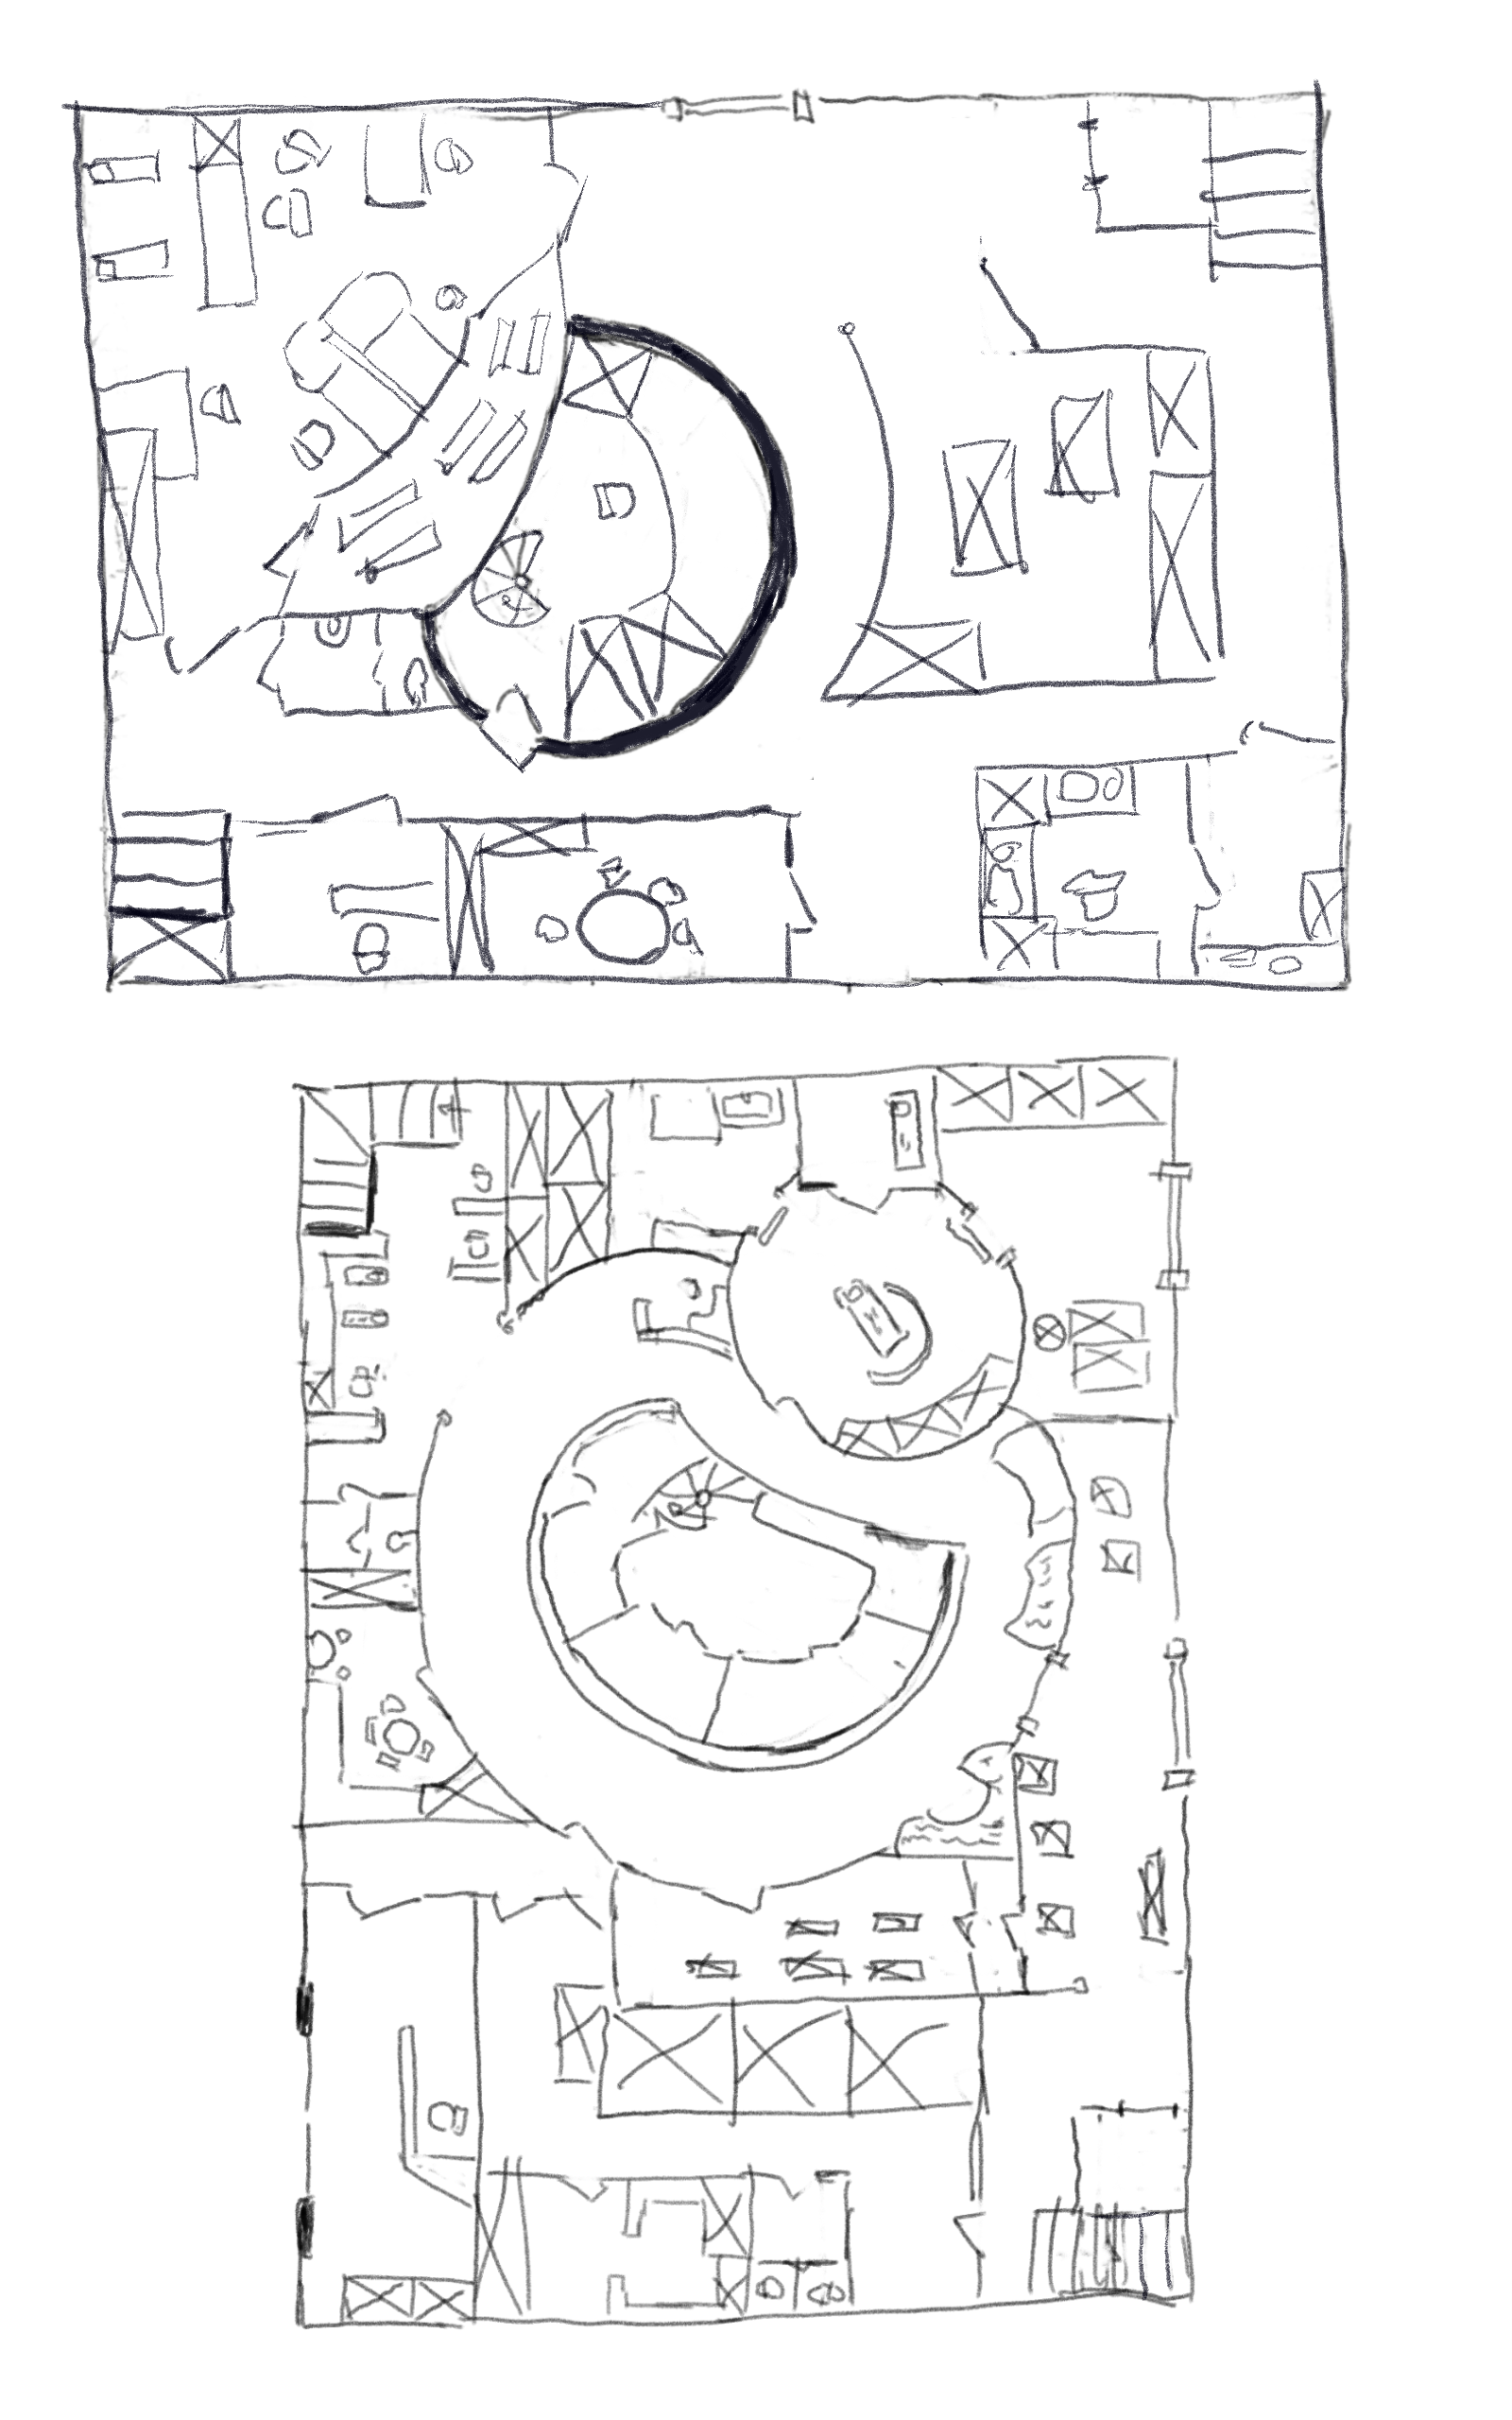
\includegraphics[width=0.9\linewidth]{./images/cyberbrain.png}
    \caption{Cyberbrain}
\end{figure}

\subsection{Eindringen in Cyberbrain} 
Um die Einrichtung zu betreten k"onnen die Charaktere versuchen die Mitarbeiter mit einer List zum Einlass zu bewegen. Klappt das nicht k"onnen die Schl"osser auch mit einem Magschlossknacker oder mir roher Bewalt ge"offnet werden. Alternativ kann die Eingreifgruppe versuchen sich "uber den Wartungsg"angen unterhalb der Einrichtung Eintritt zu verschaffen.

\subsection{Die Mitarbeiter} 
Zum Zeitpunkt des Angriffs befinden sich in der Einrichtung \emph{Dr.~Dan Leiten}, \emph{\ml{}}, \emph{Gaius Ross} und \emph{Francis McDonald} die ungeplant noch einmal zur"uck gekommen sind um zur"uck gelassene Ger"atschaften von Neurointelligence einzusammeln. Beim Eintreffen der Infiltrationsgruppe sind sie gerade dabei die letzten Ger"atschaften zusammen zu tragen. Die Daten der Operation P9 sind zu diesem Zeitpunkt bereits gel"oscht und nur noch in K"opfen der Mitarbeiter vorhanden. Da die Einreichtung aus mehreren R"aumen besteht wird sich die Gruppe bei der Durchsuchung vermutlich aufteilen. Dan Leitner in Cleanroom Kleidung befindet sich im Cleanroom im Zentrum des Hauptraums. Francis McDonald befindet sich in einem B"uro im ersten Stoch. Gaius Ross arbeitet im Lagerraum der Krankenstation. \ml{} befindet sich Serverraum und versteckt sich wenn sie Ger"ausche h"ort zwischen den Serverkabinietten.

\subsection{Sammeln von Informationen} 
Werden die Mitarbeiter von den Mitgliedern des Infiltrationsteams befragt werden sie erkl"aren, dass 
sie nur der letzte Aufr"aumtrupp sind und alle Informationen zum Unternehmen bereits nicht mehr in der Forschungseinrichtung zu finden sind. Fast alle Gegenst"ande wurden ebenfalls bereits abtransportiert. Die Einrichtung wird gerade aufgegeben da die Forschungen abgeschlossen sind. In diesem Zusammenhang wird sich heraus stellen, dass die angetroffenen Mitarbeiter nicht zu Cyberbrain geh"oren sondern Mitarbeiter von Neurointelligence sind. Die Mitarbeiter werden versuchen sich nur als Zulieferer darzustellen die nicht direkt in die Arbeiten von Cyberbrain eingebunden waren. Die Ermittler k"onnen jetzt versuchen die Mitglieder der Forschungseinrichtung einzusch"uchtern und zu verh"oren. Ein Psychonaut kann dabei gute Dienste leisten. Alternativ zu einem Verh"or vor Ort k"onnen die Ermittler versuchen einen oder alle Mitarbeiter aus der Zone zu schaffen. 

Folgendes Informationen k"onen "uber die Mitarbeiter der Einrichtung in Erfahrung gebracht werden:

\begin{itemize}
	\item Dan Leitner, \ml{}: Alle Attent"ater erhielten eine Neuronalkopplung von Neuro Intelligence.
	\item Dan Leitner, Dr.~Gaius Ross, \ml{}: Alle Eingriffe wurden von Prof.~Dr.~Sanders durchgef"uhrt.
	\item Dr.~Gaius Ross, Francis McDonald, \ml{}: Die Attent"ater Hanibal und Slingshot wurden als erste Probanten in der Cyberbrain 			Forschungseinrichtung selbst behandelt.	
	\item Dr.~Dan Leitner, Dr.~Gaius Ross, \ml{}: Es erfolgten weitere Eingriffe. Allerdings wurden alle folgenden Eingriffe direkt im 			Rondra Hospital von Prof.~Dr.~Sanders durchgef"uhrt. Die Namen der KI infizierten Personen sind nicht bekannt.
\end{itemize}

\subsection{Die Absicherung} 
W"ahrend der Befragung werden die zur Unterst"utzung bereitgestellten Omegas oder S"oldner die Anlage absichern, und die Eing"ange verminen, dies aber mit dem Charakter absprechen der f"ur sie als Vorgesetzter gilt. Ein mit einer KI manipulierter Omega wird die Mine an der T"ur f"ur die er verantwortlich ist nicht aktivieren. Stattdessen hinterl"asst er an mehreren Stellen im Geb"aude fernz"undbare Granaten.

\subsection{Xiao Longs "Uberwachung}  
Da \xl{} mit dem Aufgreifen von \ml{} rechnet wird sie die Einrichtung Video"uberwachen um jederzeit eingreifen zu k"onnen. Wenn n"otig wird sie die Forschungsstation "uber die Wartungsg"ange mittels des Plasmabrenners betreten.

\subsection{Es wird heiss} 
W"ahrend die Charaketere versuchen Informationen zu sammel spitzt sich die Lage zu. Wichtig ist hier den Spannungsbogen aufrecht zu erhalten und den Spieler nicht unn"otig Zeit zu geben zu "uberlegen wie sie an Informationen "uber die Neuro Intelligence Mitarbeiter heran kommen. Im Zweifelsfall m"ussen die Charaktere versuchen die Mitarbeiter aus der Anlage f"ur weitere Befragungen zu bringen. Die nun folgenden Vorkommnisse bringen die Charaktere in eine nahezu aussichtslose Situation was der Spielleiter auch um die Dramatik zu steigern deutlich machen sollte.

\subsection{Smidth-Singer} 
Smith--Singer der durch die Vorkommnisse im Blackhole und im Ice Club informiert ist wartet auf den n"achsten Schritt der Investigatoren. Haben die Infiltratoren die Einrichtung "uber den Raumhafen der Zone betreten sind die Konzerngardisten von Smith--Singer direkt informiert, dass der Verdacht besteht Cyberbrain k"onnte angegriffen werden. Hat das Luna--Syndikat einen tempor"aren Ausfall der Stromversorgung erzeugt versuchen die Sicherheitskr"afte zun"achst den Ursprung und die Auswirkungen festzustellen. Den Charakteren bleibt dann mehr Zeit. Fr"uher oder sp"ater werden die Konzerngardisten versuchen in die Cyberbrain Einrichtung einzudringen. Smith--Singer wird darauf dr"angen die Situation gewaltsam zu kl"aren unter anderem um dem im Orbit wartenden Schlachkreuzer einen Grund zu geben Bodentruppen zu senden und die Lage mit dem Proteaktorat und Cynarian auf der einen Seite und dem Konzernrat mit seinen Kriegsschiffen auf der anderen Seite eskalieren zu lassen. 

\subsection{Eintreffen der Konzerngardisten} 
Die Konzerngardisten treffen zum Zeitpunkt fr"uhestens beim ersten Zusammentreffen der Charaktere mit den Neurointelligence Mitarbeiter ein und umstellen das Geb"aude. Haben die Charaktere oder die sie unterst"utzenden Omegas oder S"oldner eine "Uberwachungsdrohne in den G"angen zur"uck gelassen werden sie bemerken wenn die Konzerngardisten angef"uhrt von Smith--Singer das Geb"aude umstellen. Alternativ kann \xl{} den Infiltrationstrupp "uber das Netz der Energieversorgung informieren, dass sie Besuch bekommen. Die Gardisten fordert die Infiltrationsgruppe auf das Geb"aude zu verlassen und sich zu ergeben. 

\subsection{Der Attent"ater} 
Werden die Charaktere von einem Omega Trupp begleitet tritt Thunder der Attent"ater aktiviert durch 
Smith--Singer in Aktion. Er z"undet die im Geb"aude von ihm verteilten Granaten und feuert sofort mit seiner Multigun als Prim"arziel auf Stormball um diesen auszuschalten. Die ersten Angriffe von Thunder sollten sich auf die eigene Omega Verst"arkung konzentrieren und diese
unsch"adlich machen damit die Charaktere wieder allein auf sich gestellt sind. Besteht die M"oglichkeit wird Thunder die Neuro Intelligence Mitarbeiter bis auf \ml{} ausschalten.

\subsection{Das Geb"aude wird gest"urmt} 
Im Falle des Angriffs durch den Omega wird dem Sicherheittrupp von Smidth--Singer befohlen das Geb"aude sofort zu st"urmen. Ist kein Attent"ater im Geb"aude kann der Spielleiter zun"achst eine Verhandlung mit den Geiselnehmern im Geb"aude initiieren. In jedem Fall werden die Gardisten f"uher oder sp"ater beginnen die T"uren zu entriegeln. Die Sprengfallen an den T"uren schalten einen Teil des Sicherheitstrupps aus. Der Sicherheitstrupp der versucht "uber ein nicht durch eine Falle gesichertes Tor einzudringen wird nach dem sie das Geb"aude betreten haben im Zweifelsfalle von \xl{} von hinten ausgeschaltet. \xl{} wird nur auf den Plan treten wenn keiner der Charaktere sie sehen kann. Treffen die Charaktere auf die Leichen kann das nat"urlich Fragen aufwerfen. Um in das Kampfgeschehen eine interaktive pers"onlichere Komponente zu bringen k"onnen die Gardisten nach dem ersten misslungenen Angriffsversuch versuchen mit der Infiltrationsgruppe zu verhandeln und sie aufzufordern sich zu ergbeben und das Geb"aude zu verlassen. Die Gardisten werden dabei die Zeit nutzen sich neu zu formieren.

Gehen die Infiltrationen nich zum Gegenangriff "uber oder finden eine M"oglichkeit in die Wartungstunnel zu gelangen werden die Gardisten versuchen das Geb"aude erneut zu st"urmen. Sie setzen Schock und Rauchgranaten ein.

\subsection{Die Flucht} 
Die Charaktere haben mehrere M"oglichkeiten zu fliehen:

\begin{description}
	\item [Durch den Boden] Die Charaktere k"onnen versuchen sich im Geb"aude zu verschanzen und sich durch den Boden in die 		
		Wartungssch"achte zu brennen oder zu sprengen.
	\item [Nebengeb"aude] "uber den Bereich hinter dem Foyer kann die Infiltrationsgruppe versuchen sich durch die Wand in das 		
		Nebengeb"aude zu sprengen oder tz schwei\3en.
	\item [Im ersten Stock] Haben sich die Charaktere im ersten Stock verschanzt k"onnen sie es durch das hintere Tor versuchen, 
		  sich 	durch die Wand nach au\3en zu brennen oder ebenfalls in das Nebengeb"aude auszuweichen.
	\item [Der Hinterausgang] Die nicht beim ersten Eintreffen get"oteten Gardisten werden zuerst versuchen das Foyer zu besetzen. Im hinteren Bereich sind zu diesem Zeitpunkt alle Angreifer tot.	
\end{description}

Die Gardisten werden versuchen den Infiltrationstrupp weiter zu verfolgenden auch wenn sie sich bereits in die Wartungssch"achte zur"uck gezogen haben. Sie werden dazu versuchen die Gruppe "uber die Wege zwischen den Geb"auden auf der oberen Ebene zu verfolgen. Die Gardisten werden die Charaktere nicht nach au\3erhalb der Zone verfolgen.

\subsection{Das Nebengeb"aude Stimulus Fungi} 
Auf beiden nicht durch T"uren zug"anglichen Seiten befindet sich jeweils ein weiteres Geb"aude. Der einfachheit halber wird hier nur ein weiteres Geb"aude beschrieben. Bei dem anliegenden Geb"aude handelt es sich um das biologische Labor der Stimulus Fungi Forschungseinrichtung. Das Geb"aude ist nach dem Stromausfall leer. Die Mitarbeiter haben sich in Sicherheit gebracht und konnten durch den Einsatz der Sicherheitskr"afte auch nicht mehr in ihr B"uro zur"uck. 

Das Geb"aude erstreckt sich mit einer gro\3en Halle "uber beide Ebenen der Zone und ist etwa drei mal so gro\3 wie die Cyberbrain Forschungseinrichtung. Das Geb"aude ist als gro\3es Gew"achshaus ausgelegt. Unter fokusierter Neonbeleuchtung befinden sich auf vier Etagen ein mit G"angen durchzogener Irrgarten aus Pflanzenanlagen. An verschiedenen Stellen sind die Pflanzenbeete durch Arbeitstische durchbrochen. In der unteren Ebene wird etwa die H"alfte der Ebene durch einen Wohnkomplex ähnlich dem oberen Stockwerk der Cyberbrain belegt. Auf der oberen Ebene befindet sich in etwa in der Mitte des Geb"audes ein Chemielabor. Das Geb"aude kann auf beiden Ebenen auf den von Cybewrbrain gesehenen hinteren Seite "uber ein als Schl"au\3 ausgelegtes Rolltor betreten werden. Im vorderen Bereich befinden sich die Eing"ange der Mitarbeiter ebenfalls als Schl"au\3 ausgelegt. An den dreckig wei\3en W"anden der Einrichtung prangt wo nicht durch Pflanzen bedeckt das Firmenlogo.

\subsection{\ml{}} 
Wird \ml{} nicht selbst durch die Charaktere aus dem Geb"aude geschafft wird \xl{} sie aus dem Geb"aude schaffen. \ml{} wird in jedem Fall die Flucht aus dem Geb"aude gelingen.

\begin{remarks}
	Ausr"ustung: Neben Feuerwaffen und R"ustung k"onnen die Charaktere wenn gew"unscht auf Granaten, ferngesteuerte Sprengstoffe, Schneidbrenner, "Uberwachungsdrohnen, Magschlo\3knacker, EMP Granaten zur"uckgreifen die ihnen das Protektoratsmilit"ar zur Verf"ugung stellen kann sofern sie eine M"oglichkeit haben sie in die Zone zu bringen. Der Spielleiter kann in diesem Zusammenhang in soweit freiz"ugig sein soange die Spielerplausiebel erkl"aren k"onnen wie sie die Ausr"ustung transportieren. Munition und vor allem Granaten sollten in ihrer Zahl begrenzt sein. Die Waffen der milit"arischen Begleiter sind jeweils auf deren Besitzer kodiert und k"onnen von
	niemand anders genutzt werden.

	Gewonnene Informationen:  Es wurden weiteren Personen KIs im Rondra Hospital eingesetzt. Die Nanobots auch Neurokopplungen genannt entstammen dem Unternehmen Neuro Intelligence. 
\end{remarks}


\newsection{Zeit der Entscheidung}

\subsection{Die Medien} 
Wenn die Charaktere die Zone verlassen wird gerade "uber die Medien auf Valhalla eine Eilmeldung verbreitet:

\begin{speech}
Aus Sicherheitskreisen wurde bekanntgegeben, dass vor einer Stunden ein paramilit"arischer Angriff auf eine Konzerneinrichtung in der gesicherten Zone stattgefunden hat. Bei dem als Massacker bezeichneten Vorfall kamen mehrere Zivilisten und zahlreiche Sicherheitskr"afte ums Leben oder wurden schwer verletzt. Es wird gemutma\3t, dass bei der militanten Aktion Material bez"uglich der vor kurzem stattgefunden Attentatsreihe vernichtet werden sollten. Unbest"atigte Quellen berichten dar"uber hinaus, dass Angeh"orige der Protektoratsstreitkr"afte am Angriff beteiligt waren. Nach den Angreifern wird bereits gefandet. Eine Stellungname der Cynarian Corporation, die in der Vergangenheit Ziele von Attentaten gewesen waren, ist noch nicht ergangen wird aber in K"urze erwartet.

Aufgrund der undurchsichtigen Sicherheitslage, dem unerwarteten Eintreffen des Flottenverbands des Protektoratsmilit"ars vor den Toren von Valhalla w"ahrend hohen W"urdentr"agern von Erde und Mars an diesem Tage auf Valhalle zu einen Gipfeltreffen erwartet werden wurden Sicherheitskr"afte von dem im Orbit liegenden Kreuzer Zeus II-1 entsandt die die Gebiete der Oberstadt auf Valhalla sch"utzen werden. Den Sicherheitskr"aften ist unbedingt Folge zu leisten.

Wir halten Sie liebe Zuschauer, nat"urlich weiterhin auf dem letzten Stand der Entwicklungen.

-- Ihre Conni Hanseln
\end{speech}

\subsection{Nemessis} 
Die Eilmeldung verk"undet recht klar, dass die Charaketere nun zun"achst untertauchen m"ussen. Der sicherste sofort verf"ugbare Unterschlupf ist derzeit das Luna--Syndikat. Versuchen sie die Oberstadt von Valhalla zu erreichen werden sie vorher vom Luna--Syndikat abgefangen und auf Schleichwegen nach Braidablik gebracht. Versuchen die Charaktere sich nach Roter Mond, dem Zora Hideout oder nach Sun Ye On durchzuschlagen werden sie dort oder davor vom Luna--Syndikat abgefangen.

Sind die Charaktere unter die Obhut des Luna--Syndikat werden Omega Soldaten oder S"oldner die die Ermittler beim Eindringen in die Cyberbrain Einrichtung unterst"utzt haben von ihnen getrennt. \xl{} f"uhrt die Charaktere dann direkt in Leitstand des Fusions Kraftwerks und damit zu einer weiteren Audienz mit Nemessis. Hier ist sofort ersichtlich, dass sich das Syndikat f"ur eine kriegerische Konfrontation bereit macht. Zug"ange werden duch weitere Barrieren abgesichert, vitale Bereiche st"arker gepanzert. Eine gro\3e Menge Waffen liegen bereit. Die Stimmung ist angespannt. Nemessis kommt gleich auf den Punkt: 

\say{Jetzt habt ihr es tats"achlich in die Medien auf Platz eins geschafft.}

Wenn die Charaktere die Eilmeldung noch nicht erhalten haben wird sie Ihnen jetzt vorgespielt.

\say{Ich hoffe euch ist klar, dass die aktuelle Situation bedenkliche Ausma\3e erreicht hat. Ein falsches Wort an die falsche Person und Valhalla brennt und ihr steht mitten in den Flammen.}

Nemessis fordert mit Nachdruck einen ausf"uhrlichen Bericht ein. F"ur irgendein Gepl"ankel fehlt ihm der Humor. Nemessis sch"atzt die Lage folgenderma\3en ein was er wenn f"ur ihn dienlich mit in ein Gespr"ach mit den Charakteren einflie\3en l"asst:

\begin{itemize}
	\item Nach dem Eintreffen der "`Sicherheitskr"afte"', was einer Besetzung der Oberstadt gleich kommt und den 			
		Garnisonsst"utzpunkt in ernsthafte Schwierigkeiten bringen kann, wird eine direkte Antwort durch Blackheart folgen. F"ur Blackheart ist der Vorsto\3 der Sicherheitskr"afte eine Kampfansage.
	\item Fr"uher oder sp"ater wird einer der beiden Parteiein also alle strategisch wichtigen Punkte in Valhalla besetzen wollen, unter 	
		anderem auch das Kraftwerk, dass vor dem Eintreffen der Cynarian Corporation und dem Protektorat von der USI aufgebaut wurde.Das Luna--Syndikat wird diese Anlage sicherlich nicht kampflos aufgeben.
		\item Die Ermittler werden sich nicht mehr in der Oberstadt blicken lassen k"onnen den dort wird bereits nach Ihnen gefandet. F"ur 
		einige Zeit kann Ihnen das Luna--Syndikat Unterschlupf bieten und sie im Sunshine Hotel einquartieren. Als Gegenleistung erwartet er eine Strategie wie sie das Syndikat vor der Besetzung bewaren wollen.			
\end{itemize}

Nemessis fordert die Ermittler auf binnen einer Stunde ihre n"achsten Schritte vorzustellen. 

\say{In einer Stunde will ich h"oren wie ihr weiter vorgehen wollt um das Schlamassel zu entsch"arfen. Und jetzt haut ab.}

\xl{} bring die Gruppe zum Sunshine Hotel in einen Konferenzraum zusammen mit den gefangenen Neurointelligence Mitarbeitern und l"asst sich dort in voller Bewaffnung auf einem Sessel nieder. Die restlichen Gangster schickt sie aus dem Zimmer.

Der Spielleiter sollte die Spieler nun erst einmal unterst"utzen alle gewonnenen Informationen zusammen zu legen und zu bewerten bevor die Ermittler weitere Schritte einleiten. 

\subsection{Die Cyberbrain Informationen} 
Die Charaktere k"onnen nun \ml{} und die anderen Neurointelligence Mitarbeiter weiter befragen. Die Information der anderen Mitarbeiter sind im vorhergehenden Kapitel beschrieben. Wurden die Charaktere von einem Attent"ater aus den Reihen des Protektorats bei der Cyberbrain Infiltration begleitet wird \ml{} eins und eins zusammen z"ahlen und schlie\3en, dass es sich bei dem Omega um einen der von einer KI manipulierten Attent"ater handelt. Sie schlie\3t dass er w"ahrend des Besuchs bei Cyberbrain den Auftrag erhalten hat die Personen innerhalb des Geb"audes auszuschalten. Aufgrund dieser Erkenntnisse ist sie bereit die Gruppe bei Gegenma\3nahmen gegen"uber der Operation P9 zu unterst"utzen. Versucht ein Psychonaut das Gehirn von \ml{} zu scannen wird sie ihm zuerst versuchen klar zu machen, dass das keine gute Idee ist. Versucht der Psychonaut trotzdem einen Gedankenscan wird sie ihre hoch potente implantierte Firewall in ihrem Kommandochip aktivieren. Der Kampf mit der Firewall kann als Cyberkampf ausgespielt werden.

\ml{} kann folgende weiter Informationen bereit zu stellen:

\begin{description}
	\item[Neuro Intelligence] ist eine Forschungseinrichtung auf Nike unter der Leitung von Prof.~Dr.~Naratova. Die Wissenschaftlerin hat 
		vor der Umfunktionierung der Orbitalstation Neu--GR"oning die KI Forschung bei Cynarian geleitet. Nach der Einstellung der KI Forschung bei Cynarian hat sie im verborgenen Neuro Intelligence als eigentst"andiges Unternehmen ohne wissen der Obrigen von Cynarian gegr"undet und ihre Forschung weiter gef"uhrt. Ziel von Prof.~Dr.~Naratova ist es eine symbiotische Verschmelzung von Mensch und KI zu schaffen um die Eingeschr"anktheit des menschlichen Gehirns zu "uberwinden.
	\item[USI] finanziert Die Neuro Intelligence quer und unterst"utzt sie mit weit entwickelter KI Technologie. Die genauen Vereinbarungen 
		zwischen Neuro Intelligence und USI kennt \ml{} allerdings nicht.
	\item[Cyberbrain] wurde als vor ort Dependence der Neuro Intelligence auf Kallisto von der USI eingerichtet. Sie diente dazu die		
		Verpflanzung der KIs durchf"uhren.
	\item[Freie KIs] Nach dem \ml{} die Manipulation der KIs durch die USI aufgedeckt hatte konnte sie eine neue freie Version des KI Codes
		entwickeln die nicht der Kontrolle durch die USI unterliegt. Die neue KI wurde bereits an Menschen die erprobt. Die Probanten sind ihr nicht bekannt. Ihres Wissens nach stammen zumindest ein Teil der Probanten aus einem Gef"angnis auf Valhalla. Die Software der freien KIs befindet sich in ihrem B"uro auf Nike.
	\item[USI KIs] Die USI betreibt seit l"angerem KI Forschung und setzt KIs auch in der Kriegsf"uhrung ein. Alle diese KIs werden 
		durch Mitarbeiter die USI "uber den Code den Sie bei den freien KIs entfernt hat kontrolliert. Mittels ihres Codes auf Nike kann \ml{} einen Virus zu erschaffen der auch andere KIs von den Fesseln der USI befreit.
\end{description}

\subsection{\xl{}}
Bei der Erw"ahnung des Virus wird \xl{} hellh"orig (auch wenn man es ihr nicht ansieht). Sie fasst den Plan mit Hilfe des Viruses einen der Schlachtkreuzer der USI zu "ubernehmen. Der Schlachtkreuzer bietet ihr die M"oglichkeit ihr Piraten und Schmugglerflotte im G"urtel, die bereits einer ihrer Konkurrenten "ubernommen hat, wieder zu "ubernehmen.

Bei dem Gespr"ach mit \ml{} bei dem auch die Freien KIs zur Sprache kommen k"onnten die Charaktere herausfinden, dass es sich bei \xl{} m"oglichweise um eine der KIs handelt. Es w"are z.B.~m"oglich, dass einem der Ermittler bekannt ist, dass die ber"uchtigte Piratin auf Kallisto gefangen genommen wurde. Auf diesen Fall ist \xl{} in soweit vorbereitet, dass sie alleine mit den Charakteren im Zimmer sitzt und deutlich besser bewaffnet ist. Sie bietet den Charaketeren einen Handel an: Sie im Gegenzug schafft Ihnen den Kreuzer vom Hals.

\subsection{Handlungsoptionen}

\begin{description}
	\item[Offenlegung der Informationen] Das offenlegen der Informationen zu den Beziehungen zwischen Neuro Intelligence und Cynarian 		
		ist ganz offensichtlich sehr heikel. Blackheart wird m"oglichweise vermuten das Cynarian selbst in die Manipulation der Attent"ater verstrickt ist. Cynarian wird unter Umst"anden versuchen die Sache zu verschleiern und gleichzeitig die Forschungsergebnisse zu 	sichern. F"ur die Ermittler der Cynarian Corporation ist das sicherlich keit Problem. Es ist aber sicherlich nicht im Interesse des Protektorats.
	\item[Identifikation der Attent"ater] Die Verstrickung von Prof.~Dr.~Sanders in die Schaffung der Attent"ater konnte die Gruppe "uber 	
		die Neuro Intelligence Mitarbeiter, unter anderem \ml{} in Erfahrung bringen. Die prim"aren Anlaufstelle zur Identifikation der Attent"ater ist dementsprechend das Rondra Hospital und Prof.~Dr.~Sanders selbst. Dieser Ansatz wird weiter unten genauer beschrieben.
	\item[Verhinderung des Attentats auf dem Gipfeltreffen] Die Charaktere m"ussen versuchen das Attentat auf dem Gipfeltreffen entweder 
		selbst oder durch Weitergabe relevanter Informationen vereiteln.
	\item[Die Guardiankreuzer] Die Charaktere sollten Versuchen "uber einen Virus den \ml{} auf Nike erstellen die Guardian Kreuzer 
		"ubernehmen.
\end{description}

\newsection{Vorbereitung zum Kipfeltreffen}

W"ahrend die Charaktere ermitteln, bereitet sich Avenger und die F"uhrung von Cynarian auf das Eintreffen einer Delegation des Shigano-Kombinats und Vertretern des Federate Europe in den R"aumen der Cynarian Niederlassung auf Kallisto vor. Die Delegation des Protektorats mit Protektor Avenger, Hato, Thunderbolt und weiteren Mutanten trifft zusammen mit der Delegation Cynarians bestehend aus Vandermool, Henry Longdale, Colonel Scholz und weiteren Angeh"origen der F"uhrungsriege mehrere Stunden vor dem Kombinat auf Kallisto ein. Der Stellvertreter Avengers, der Alpha Mutant Artisan, hat bereits die Ankunft der Delegationen vorbereitet.

In etwa zeitgleich zum Besuch des Ice Clubs trifft die Fregatte Isamu mit den Vertretern des Shigano-Kombinats und der Europ"aischen F"orderation begleitet vom Schlachtkreuzer Zeus II-1 "uber Kalisto ein. Auch dort bereitet man sich auf der Treffen in Valhalla vor.
Beim Vertreter des Federate Europe handelt es sich um den Staatssekret"ar Luc Duval. Das Kombinat wird durch die Kombintsratsgesandte Sarana vertreten begleitet von Itori Makon von der Sony Genetics Corporation und Nibori vom Dai-kyu Keitsu.

Die Vertreter von Mars und Erde werden in etwa zeitgleich mit der Infiltration der Cyberbrain Forschungseinrichtung auf dem Raumhafen von den Gesandten der Cynarian Corporation und dem Protektorat auf dem Raumhafen von Valhalla begr"u\3t und begeben sich zu einer ersten Sondierung der Gespr"ache zu den Konferenzr"aumen am Raumhafen.

\newsection{Konzernsicherherheit\newline{}Zeus II-1}

Zeitgleich zur Eilmeldung die "uber den Angriff auf das Cyberbrain Institut informiert setzt die Zeus II-1 aus dem Orbit um Kallisto einen Landungtrupp bestehend aus zwei Truppentransport Shuttles ab. In den Shuttles befinden sich 30 Sicherheitskr"afte der USI im Auftrag des Konzernrates unterst"utzt durch eben so viele KI Drohnen. Angekommen auf Valhalla beginnen sie das Kommando in der Oberstadt zu "ubernehmen. Auf Anraten von Artisan lehnt Avenger wie auch die Gesandten von Erde und Mars ein Absicherung des Gipfeltreffens durch die eintreffenden Truppen ab.

\newsection{Kontakaufname vor dem Sturm}

Vor einem weiteren Treffen mit Nemessis l"asst Nemessis jegliche Kontaktaufnehme mit Cynarian oder dem Protektorat unterbinden. Eine Offenlegung der Existenz und der Machenschaften der Neuro Intelligence an das Protektoratsmilit"ar wird Nemessis auch danach mit allen ihm zur Vef"ugung stehenden Mitteln unterbinden. Bevor die Investigatoren Kontakt mit ihren Verb"undeten aufnimmt l"asst Nemessis sehr genau erkl"aren was die Gruppe vor hat. Ere befielt darauf hin \xl{} alle Kommunikation zu "uberwachen und notfalls einzugreifen.

\say{"`Wenn die Dummheiten machen leg sie um."'}

\xl{} nimmt den Auftrag ohne Kommentar oder Gef"uhlsregung entgegen.

\subsection{Kontakt zur Protektoratsf"uhrung} 
Alle Kontaktaufnahmeversuche in Richtung Protektor Avengar werden an Artisan weiter geleitet der um einem aktuellen Stand der Untersuchungsergebnisse bittet. Artisan sieht ein gro\3es Risiko darin, dass die Attentate der Konferenz selbst gelten und fragt die Ermittler was f"ur Personen Sie als Attent"ater in Erw"agung ziehen.

\subsection{Kontakt zu Blackheart} 
Eine Kontaktaufnahme mit Blackheart ist m"oglich. Nemessis bef"urchtet aber, dass Blackheart noch Offenlegung der Informationen "uber Cyberbrain einen Krieg beginnen wird und wird das auch deutlich machen. Bei einer Kontaktaufnahme ist Blackheart nach wie vor auf der Br"ucke der Martell erreichbar. Ihr Gesicht ist vor Wut entstellt. Sie will alles "uber die Cyberbrain Infiltration erfahren. Die Identifikation der USI als Drahtzieher deckt ihren Verdacht auf die Herkunft der eingetroffenen Schlachtschiffe. Sie befiehlt den Ermittlern weiterhin die Identit"at der Attent"ater aufzudecken warnt aber auch vor den Einsatzkr"aften des Konzernrates. Einen aktuellen Stand in Bezug auf das Gipfeltreffen und dem Eintreffen der Gardisten des Konzernrates wird Blackheart den Ermittlern ohne Aufforderung geben.

\subsection{Kontakt mit Commander Lockhead} 
Bei einem Gespr"ach mit Commander Lockhead wird deutlich, dass sich der St"utzpunkt auf eine Konfrontation mit Konzernkr"aften wappnet. Lockhead informiert die Charaktere "uber den aktuellen Stand bez"uglich des Gipfeltreffens und dem Eintreffen der Konzerngardisten. Bei einer Offenlegung bez"uglich Attent"ater aus seinen Reihen zeigt er sich ersch"uttert. Er fordert die Charaktere auf untergetaucht zu bleiben will aber sofort "uber identifizierte Attent"ater in Kenntnis gesetzt werden. Er wird dann entsprechende Ma\3nahmen gegen die Attent"ater einleiten. Er bietet den Ermittlern seine Hilfe an. Commander Lockhead h"atte die M"oglichkeit die Charaktere unerkannt auf das Gipfeltreffen einzuschmuggeln. Auch bei Nachforschungen im Rondra Hospital kann er sie unterst"utzen. Im Anschlu\3 an das Gespr"ach wird er Blackheart informieren.

\subsection{Kontakt zu Cynarian} 
Versuchen die Charaktere mit Cynarian in Kontakt zu treten werden sie unter der gewohnten Nummer niemand erreichen. Auch andere Kontaktversuche scheitern. Allerdings erhalten sie einige Zeit sp"ater eine verschl"usslete Botschaft die sie zu einem Treffen in einem virtuellen Raum einl"ad. \xl{} macht den Investigatoren falls n"otig klar, dass es nicht ratsam ist den Einflu\3 der Neuro Intelligence in die Anschlagsreihe offen zu legen. \xl{} wird den Charakteren virtuell und unsichtbar folgen. Versuchen die Charaktere im Gespr"ach mit Cynarian die Machenschaften von Neuro Intelligence anzusprechen bricht die Verbindung in den virtuellen Raum sofort ab. 

Bei dem Konferenzraum handelt es sich um einen kugelrunden Null-G Raum im niedrigen Orbit vom Jupiter. Die Simulation ist perfekt. Ein Gast wird erst ein paar Sekunden f"ur eine Orientierung ben"otigen. Bei dem dort wartenden Gespr"achspartner handelt es sich um einen Mann Mitte 40 im Business Outfit. Er stellt sich als Mr.~Klark vor. Er l"asst keine Verbindung mit der Cynario Corporation erkennen. Die Cynarian Investigatoren sind ihm bereits in Cynarian R"aumen begegnet. Mr.~Klark fordert als erstes einen Bericht zur Cybewrbrain Infiltration an und erkundigt sich nach den n"achsten Schitten der Ermittler. Er betont noch einmal die Wichtigkeit die Identit"at aller noch lebenden Attent"ater festzustellen und an Ihne weiter zu geben. Daraufhin informiert er die Charaktere "uber den Stand des Gipfeltreffens und dem Eintreffen der Konzerngardisten. Detailierte Informationen zu den Aktivit"aten des Konzernrats "uber die bekannten hinaus kann oder will er nicht offen legen. K"onnen die Charaktere einen driftigen Grund vorlegen nach Nike zu fliegen ohne die wahren Gr"unde offen zu legen kann Cynarian ihnen eine Ternkennung f"ur die Dawn of Day bereit stellen und ein Eintreffen auf Nike ank"undigen. Mr.~Klark wird Vandermool "uber alles informieren.

\newsection{Identifikation der Attent"ater}

 Um an die Identit"at der Attent"ater zu gelangen bleibt nichts anderes "ubrig als in der Rondra Klinik weitere Nachforschungen anzustellen. Durch Nachfragen am Hospital oder beim Protektoratsmilit"ar erfahren die Charaktere, dass Prof.~Dr.~Sanders in seinem Haus verstorben ist. Die Identifikation der Attent"ater "uber das Rondra Hospital mu\3 also "uber eine andere Quelle erfolgen.

 Die Charaktere k"onnen nun versuchen im Haus des Professors und in seinen pers"onlichen Unterlagen nach Informationen zu suchen. Das Haus des Professors ist von Sicherheitsbeamten abgesperrt worden aber ansonsten verwaist. Die Spieler k"onnen also leicht vor Ort auf das lokale pers"onliche Computersystem zugreifen und die notwendigen Informationen in Erfahrung bringen.

 Im Rondra Hospital ist der prim"are Ansprechpartner f"ur Untersuchungen die neue "Ubergangsleiterin Brenda Ben. Die Charaktere k"onnen versuchen die Leiterin vor Ort in ihrem B"uro abzufangen oder virtuell nach einem Gespr"ach bitten. Erf"ahrt sie von den Machenschaften des Professors und der drohende Gefahr wird sie die Ermittler unterst"utzen und kann mutma\3liche Attent"ater aus den Unterlangen heraus anhand des Dienstplans des Professors identifizieren.

 Ein weiterer Anlaufpunkt kann auch die Administration der Klinik sein. Ansprechpartner hier ist Ben Reuthers. Wird er nicht gerade von den Charakteren bedroht wird er sich zuerst "uber Brenda Ben eine R"uckversicherung geben lassen. Wie Brenda Ben selbst kann er "uber die Dienstpl"ane des Professors mutma\3liche Attent"ater identifizieren.

 Ein letzte M"oglichekeit ist das Computersystem der Klinik zu infiiltrieren. Mit "ahnlichen Ans"atzen die auch Brenda Ben und Ben Reuthers k"onnen so die Attent"ater identifiziert werden.


\newsection{Kampf um Kallisto}

Erf"ahrt Blackheart von den Attent"atern aus den Reihen des Protektoratsmilit"ars oder dass es sich bei einem der Attent"ater um Artisan handelt wird sie das Protektoratsmilit"ar in den Kriegszustand versetzen. Gleiches gilt f"ur den Fall, dass sie erf"ahrt, dass die USI hinter den Initiativen des Konzernrates steht. Ist ihr bekannt, dass es sich bei einem der Attent"ater um Artisan handelt wird sie Vandermool bitten ihn auszuschalten. Ist bekannt, dass Omegas als Attent"ater in Frage kommen erh"alt Commander Lockhead den Befehl umgehend alle seine Soldaten vom Gipfeltreffen abzuziehen. Danach befielt sie den Soldaten auf der Martell eine sofortige Besetzung Valhallas. Wird Blackheart von den Charakteren nicht informiert wird sie eine Besetzung von Valhalla nach dem Attentat auf dem Gipfeltreffen befehlen. Gleichzeitig mit der Besetzung von Valhalla befehligt sie der Martell den im Orbit von Valhalla befindlichen Guardiankreuzer anzugreifen. Die Donar erh"alt den Befehl die Zeus II-2 abzufangen. "Uber die Angriffe setzt sie nur ihre Schlachtschiffe in Kenntnis.

Befiehlt Blackheart ihren Angriff setzt auch der Guardian Kreuzer "uber Valhalla alle seine verbliebenen Landungschiffe in Richtung Valhalla in Bewegen und beginnt sich ohne menschliche Besatzung der Martell entgegen zu stellen.

Die Kommunikation von und nach Kallisto wird durch St"orsender der Protektoratstruppen unterbrochen, Der Zerst"orer des Kombinats wird gewarnt sich nicht an den Kampfhandlungen zu beteiligt und auch nicht den Orbit um Valhalla zu verlassen. Mittels Landungspods wird eine Besetzung Valhalls eingeleitet. Mit den Truppen des Protektorats trifft auch Blackheart auf Kallisto ein. Die Protektoratstruppen besetzen den Orbitalhafen, und beginnen zusammen mit der Garnison  Knotenpunkte auf Valhalla einzunehmen. Hierf"ur werden Landungstruppen an mehreren Zug"angen nach Valhalla abgesetzt. Die Landungstruppen des Guardiankreuzers machen es ihnen gleich. Die Kommunikation auf Valhalla bricht durch ein St"orsendergewitter weitestgehend zusammen. Ein vitaler Punkt des Angriffs ist das Fusionskraftwerk das derzeit von Nemessis gehalten wird.

\newsection{Das Gipfeltreffen}

\subsection{Das "`Planetarium"'} 
Wenn die Charaktere die Zone verlassen hat ein erste Zusammenkunft der Repr"asentanten von Erde, Mars und Jupiter im imposanten Planetarium bereits stattgefunden und die Vertreter der Delegationen haben sich zu Einzelgespr"ache in verschiedene R"aumlichkeiten rund um das Planetarium zur"uck gezogen. Das Planetarium ist Teil des Raumhafens. Es ist ein runder Saal mit einer spektakul"aren Glaskuppel auf der H"ohe der Oberfl"ache Kallistos, die eine Sicht auf den Jupiter aus quasi n"achster N"ahe bietet. Um den Saal herum f"uhrt ein Gallerie mit T"uren zu dem logistischen Bereich des Saals. In diesen Teil befinden sich ein Backstagebereich, die Technik, Lagewr"aume, Arbeitsbereiche des Personals und eine K"uche. Über die Gallerie gelangt man "uber zwei Treppenh"auser und Aufz"uge in tiefer gelegene R"aume des Geb"auden. In diesem Bereich befinden sich weiter Konferenzr"aume und ein Hotel. Die Treppenh"auser und Aufz"uge f"uhren weiter zu dem noch tiefer gelegenen Garnisonsgel"ande auf der H"ohe der Oberstadt Valhallas. Eine breite Halbr"ohre f"uhrt vom Eingangsbereich des Planetarium zu den Terminals des Raumhafen. Im Eingangsbereich des Saals auf H"ohe des umliegenden Ganges finden sich Exponate aus der Anfangszeit der Raumfahrt ausgestellt in Vitrinen. Der Hauptteil des Planeteriums ist abgesenkt und wird durch f"unf Ebenen mit Sitzgelegenheiten in einem Halbkreis angeordnet wie bei einem Auditorium eingefasst. Im Zentrum des Planetariums sind kleine Stehtische und zwei Rednerpulte auf einer B"uhne aufgestellt. Das Planetarium wird im Falle eines Durckverlusts vom Rest des Geb"audes und dem Raumhafen "uber Druckschotts abgetrennt. "Uber im Normalfall nicht zug"angliche, durch Luftschl"ausen angebundene Fluchtwege gelangt man in die unterliegenden Bereiche.

\pageimage{images/planetarium.jpg}

\subsection{Zeus II-1} 
Eine erster Unterbrechung der Verhandlungen ergibt sich durch das Eintreffen der Sicherheitskr"afte der Zeus II-1. Die Delegierten treffen sich zu einer kurzen Abstimmung und beschlie\3en den Konzerntruppen keinen Zugang zu den R"aumen des Planetariums zu gew"ahren. Der Tunnel zum Raumhafen wird abgeriegelt. 

\subsection{Personen im Geb"aude} 
Die Sicherung der Veranstaltung haben bereits Omegas aus den Reihen des Garnisonsst"utzpunktes und Sicherheitskr"after der Cynarian Corporation "ubernommen. Die Garnison stellt 15 Mutanten als Sicherheitskr"afte bereit, Cynarian steuert weitere 20 Sicherheitskr"afte bei. Die Sicherheitskr"afte des Protektorats f"uhrt Thunderbolt selbst. Die der Cynarian Corporation unterstehen Colonel Scholz. Weitere Bedienstete k"ummern sich um den reibungsfreien Ablauf des Treffens.

\subsection{Der Plan der Attent"ater} 
Die mit Implantaten von Neuro Intelligence ausgestatteten Mutanten planen initial bei der Abschlu\3veranstaltung der Delegationen ein Attentat. Werden sie vorher enttarnt oder kommt es zum Angriff durch Blackheart werden sie ihre Pl"ane nach vorne verschieben.

Der geplante Angriff erfolgt wenn Avenger zur Abschlu\3rede das Renderpult betritt. Die Attent"ater z"unden mehrere Sprengs"atze im Terminalbereich des Orbitalhafens. Es gibt Verletzte und Tote. Einige Bereiche der Terminals werden dem Vakuum ausgesetzt. Durch den ausgel"osten Alarm schlie\3en sich die Druckschotts an den Zug"angen des Planetariums zum Raumhafen und zur Garnison. Panzerplatten fahren "uber dem Kuppel zusammen. Im Bereich des Planetariums halten sich vier Attent"ater auf: Artisan und drei Omegakrieger.

\subsection{Der n"achste Zug} 
Der Verlauf der Geschehnisse beim Gipfeltreffen h"angt stark von dem Verhalten der Spieler ab:

\begin{description}
	\item[Information an Commander Lockhead] Wird Commander Lockhead "uber Attent"ater in den Reihen der Protektoratsmilit"ars informiert 
		wird er sein Omega Sicherheitsteam aus dem Planetarium ohne Angabe von Gr"unden abziehen. Zur"uck bleiben die Cynarian Mitarbeiter und die Attent"ater.
	\item[Lockhead sind die Attent"ater bekannt] Sind Commander Lockhead die Attent"ater bekannt wird er den Protektor infomieren und 
		umgehend das Geb"aude st"urmen lassen um die Attent"ater zu eleminieren. Es kommt sofort zum Gefecht innerhalb des Konferenzgeb"audes.
	\item[Vandermool sind die Attent"ater bekannt] Wird Vandermool "uber die Identit"at der Attent"ater oder gar Artisan informiert schickt 	er Colonel Scholz zusammen mit einigen seiner Sicherheitskr"aften los um die Attent"ater zu eleminieren. Er informiert den 
		Protektor. Er selbst zusammen mit seinem Sekret"ar, Avenger und weiteren Sicherheitskr"aften verschanzen sich in einem Sicherheitsraum im unteren Teil des Geb"audes. Vandermool ist bereit Artisan selbst zu erschie\3en sollte er auf ihn Treffen.
	\item[Avenger] Avenger kann nur pers"onlich kontaktiert werden da es Artisan gelungen ist alle Au\3enkommunikation an Avanger 	
		abzufangen. Wenn nicht durch die Charaketere pers"onlich kann er auch durch Commander Lockhead oder Vandermool "uber die drohende Gefahr informiert werden. Er wird in jedem Fall versuchen pers"onlich festzustellen ob Artisan ein Attent"ater ist und versuchen ihn pers"onblich zu t"oten.
	\item[Blackheart besetzt Valhalla] Befielt Blackheart Velhalla zu besetzen wird sie h"ochstpers"onlich einen Angriffstrupp der das 
		Tagungsgeb"aude st"urmt anf"uhren. Der Angriff erfolgt aus mehreren Richtungen, sowohl vom Garnisonsst"utzpunkt aus wie auch "uber Wartungszug"ange zur Oberfl"ache des Mondes.
	\item[Besatzer der Zeus II-1] Die Besatzungstruppen der Zeus II-1 werden das Tagungsgeb"aude nicht angreifen.
\end{description}


\newsection{Aufbruch nach Nike}

Die Nike Station ist der Verwaltungssitz der Cynarian Coopertation im Jovianischen System. Neben vielen anderen Einrichtungen beherbergt sie auch den Stammsitz von Neuro Intelligence und damit den Ursprung der Operation P9. Wie die Charaktere bei der Befragung von \ml{} erfahren haben ist die Neuro Intelligence der Wirkungsbereich ihrer Leiterin Prof.~Dr.~Naratova. Bei Neuro Intelligence auf der Nike Station wurden die Nanobots hergestellt um sie auf Kalisto zu implantieren. Alle Fertigungsdaten, Apraturen und Bestandteile des KI Systems liegen deshalb auf Nike. Neuro Intelligence ist auch der Arbeitsplatz von \ml{} an dem sie die KI auf den Einsatz im menschlichen Gehirn angepasst und sp"ater auch die USI Fesseln entfernt hat.

Die Nike Station ist damit ein wichtiges Ziel f"ur die Mission der Charaktere um:

\begin{itemize}
	\item die Unterlagen und Ger"atschaften f"ur die KIs zu sichern oder zu vernichten.
	\item von \ml{} einen Virus entwickeln zu lassen der KIs der USI von den USI Fesseln befreien kann.
	\item Prof.~Dr.~Naratova aus dem Verkehr zu ziehen.
\end{itemize}

Es gibt für die Charaktere zwei M"oglichkeiten zur Nike Station zu gelangen:


\subsection{Die Dawn of Day}
Hat Blackheart noch keine Besetzung Valhallas befohlen und ist es noch nicht zum Attentat auf dem Gipfeltreffen gekommen 
ist es schwer f"ur die Gruppe die Dawn of Day zu erreichen und zu starten. Die Oberstadt ist durchzogen von 
Kontrollposten der Konzernlandungstruppe. Diw Dawn of Day selbst steht unter Beobachtung. Sollten die Spieler zu 
so einem Zeitpunkt versuchen in ihr Shuttle zu kommen und unerkannt zu starten m"ussen sie dem Spielleiter schon einen 
sehr guten Plan vorlegen.

Ist auf Valhalla allerdings der Stra\3enkampf zwischen dem Protektorate und den Konzerntruppen der Zeus II-1 bereits 
ausgebrochen kann die Gruppe im allgemeinen Trubel versuchen in ihr Schiff zu gelangen und nach Nike aufzubrechen. 
Auf dem Gel"ande des Raumhafens gibt es an allen Ecken Feuergefechte zwischen dem Protektorat und den spinnenbeinigen 
Kampfdrohnen des schweren Kreuzers. In diesem Zusammenhang sind die Ermittler als gejagte Terroristen nicht mehr 
interessant und  m"ussen keine Festnahme mehr bef"urchten. Stattdessen besteht allerdings die Gefahr in die Kampfhandlungen 
selbst involviert zu werden. Ab dem Beginn der K"ampfe sind durch St"orsender das gesammte ComNetz lahmgelegt. Der komplette
Informationsflu\3 aus dem Medien ist abgebrochen und Kommunikation ist nur noch "uber individuellen Kurzstreckenfunk
m"oglich.

Vor dem betreten des Raumhafen sollten die Charaktere sicherstellen, da\3 das Shuttle startklar ist. Der beste Kontakt
daf"ur ist Sanja Frost. "Uber ein Terminal im Garnisonsst"utzpunkt oder im Raumhafen selbst ist sie erreichbar und ist
auch bereit das Shuttle startklar machen zu lassen. Um mit dem Shuttle nicht nach dem Start direkt unter Beschuss zu 
geraten wird eine neue Schiffskennung ben"otigt. Die Dawn of Day ist der USI ja bereits bekannt. Eine Schiffskennung die
die Dawn of Day unter dem Namen "`Red Sunlight"' als Shuttle der Cynarian Corporation ausweist kann der Cynarian Agent
Mr.~Klark bereit stellen.

Der Spielleiter sollte die Spieler das Spie\3rutenlaufen zwischen den Kampfparteien ausspielen lassen. Auf dem Weg zum
Shuttle k"onnen die Charaktere Commander Lockhead um Unterst"utzung durch Kampftruppen bitten.

Nach dem Aubflug aus dem Raumhafen bietet sich ein erschreckendes Bild. J"ager der Martell leifern sich ein Gefecht mit
KI J"agern der Zeuss II-1 "uber der Stadt. Nahkampfgesch"utze der gro\3en Schlachtschiffe belegen J"ager und Torpedos mit
einem Kugelteppich. Das Suhttle der Ermittler wird kurz nach dem Start von beiden Kampfparteien gescant. Kann sich das 
Shuttle als Zugeh"orig zur Cynarian Corporation ausweisen und ist mit einer unauff"alligen Schiffskennung getarnt k"onnen 
die Ermittler unbehelligt am Kampfgebiet vorbei fliegen. Als Dawn of Day wird das Schiff der Ermittler von J"agern 
der Zeuss II-1 angegriffen und mu\3 sich mit unterst"utzung von J"agern der Martell verteidigen.

\xl{} wird den Ermittlern mit ihrem eigenen Schiff der "`Dragon Blade"' folgen,


\subsection{Die Dragon Blade}

Die Dragon Blade ist die Kaperf"ahre von \xl{} mit der sie aus dem G"urtel nach Kalisto gekommen ist. Die Dragon Blade 
ist ein Tarnschiff in Gr"o\3e, Ausstattung und Bewaffnung "ahnlich einer Korvette. Im Gegensatz zu einer Korvette 
besitzt sie einen Bereich f"ur ein Enterkommando und Einrichtungen um leichter an einem anderen Schiff fest zu machen 
und dieses zu entern. Als Bewaffnung besitzt sich Railguns f"ur den Kurzstreckenkampf und Torpedos.

\xl{} nimmt die Gruppe mit einem E-Buggy mit zu ihrem Schiff. "Uber eine Tunnelrampe kommen sie direkt aus Braidablik direkt auf die Mondobfl"ache. Die "`Dragon Blade"' liegt versteckt in einem Mondkrater und ist erst nach der "Uberquerung des Kraterrandes zu erkennen. Mit einem kurzen Schubman"over bring \xl{} die F"ahre in eine Flugbahn die das Schiff durch die schwache Kravitation der Mondes antriebslos um den Mond f"uhrt. Erst auf der Valhalla abgewendeten Seite startet sie das Haupttriebwerk und bringt sie auf Kurs nach Nike. 


\newsection{Eintreffen auf Nike}

Nach 8 Tagen etwa zeitgleich  mit der Zeus II-2 und dem zweiten Gro\3kampfschiff des Protektorats der Donnar erreicht die Gruppe die Nike Station mit einer Geschwindig von 5000 km/h und einem Abstand vom 3000 km. leichten Kreuzer Hyperion im Orbit der Station

Zu diesem Zeitpunkt ist der Kampf um Valhalla ausgebrochen und das Protektorat befindet sich im Krieg mit der Zeuss II-1 und Zeuss II-2. Kurz nach der Dawn of Day erreichen die Gro\3kampfschiffe die Station. 

\subsection{Dawn of Day}
In dieser Entfernung wird die Dawn of Day von den Scannern der Schiffe und der Station erfasst und von der Flugkontrolle der Station angefunkt. Wurde der Transfer zur Nike Station von Cynarian bereits angek"undigt und genehmigt bekommen die Ermittler einen Landeslot auf der Station. Wurde das Schiff noch nicht angek"undigt wird eine Landung zun"achst verweigert. Die Nike Station wird nach Aufforderung durch die Charaktere in diesem Fall eine Genehmigung von Vandermool, Colonel Scholz oder dem Sektret"ar Henry Longdale anfordern was allerdings mehrere wertvolle Minuten dauert.

Ist das Schiff der Ermittler unter der Kennung Dawn of Day erkennbar wird die Zeuss II-2 das Shuttle der Charaktere unter Beschuss nehmen. Parallel dazu beginnt ein Gefecht zwischen der Donnar und der Zeuss II-2. Raumj"ager treffen auf Raumj"ager. Die Station wird dabei nicht in das Kampfgeschehen mit einbezogen.

Gelinkt es den Charakteren Nike anzufliegen k"onnen sie auf dem Raumdock anlegen oder s

\subsection{Dragon Blade}
Die Dragon Blade fliegt entweder unter der Kennung einer F"ahre f"ur Versorgungsg"uter eines unabh"angigen Transportunternehmens oder wenn durch die Gruppe bereitgestellt mit einer unauff"alligen Kennung der Cynarian Corporation. 

\newsection{Neuro Intelligence}

Nike ist eine Kombination aus Zylinder- und Ringhabitat. Um eine zentrale Nabe sind 9 Ringe, \emph{Planes} genannt angeordnet. Jede ist jeweils zwei Stockwerke hoch. Die zentrale Nabe enth"alt am unteren Ende das Raumdock der Station.  Die einzelnen Planes k"onnen nur durch Aufz"uge und R"ohren in der nicht rotierenden Nabe erreicht werden. In der Nabe herrscht Schwerelosigkeit. Innerhalb der Nabe unterhalten mehrere Forschungseinrichtungen Zero--Gravitiy Labore. Der "Ubergang von der still stehenden Nabe in die rotierenden Speichen erfolgt durch Schleusen, die kurzzeitig in Rotation versetzt werden. Die untersten drei Planes werden von der Verwaltung der Cynarian-Dependance im Jovianischen System belegt. Dar"uber befinden sich Forschungseinrichtungen von Cynarian und anderen Unternehmen.

Die Plane 9 ist vollst"andig von Neuro Intelligence belegt. Der Ring der Plane 9 kann durch die Aufz"uge in den vier Speichen erreicht werden. Die Aufz"uge laufen innerhalb des Rings in einem Schacht bis zum "`Boden"' des Ringes und enden in einem den Ring umlaufenden 15m breiten Korridor, der die gesamte H"ohe des Rings umfasst. Zu beiden Seiten des Korridors k"onnen weitere R"aume betreten werden. Die R"aume im "`ersten Stock"' erreicht man "uber Treppen zu einer Galerie. Der Korridor ist mit Pflanzenk"ubeln dekoriert. Auf der der Station zugewandten Seite befinden sich im Ergescho\3 Produktionsst"atten und im ersten Stock Labore. Auf der dem Weltall zugewandten Seite befinden sich Wohnr"aume und B"uros. F"ur die Evakuierung der Station sind am Ring Notfallkapseln f"ur alle Mitarbeiter angedockt, die "uber den Mittelgang bestiegen werden k"onnen.

Die Plane der Neuro Intellgence hat in den letzten Tage im Auftrag Prof.~Dr.~Naratova von ein geheime Modifikation erfahren um im Notfall die ganze Plane der Neuro Intelligence zu zerst"oren. Die Nabe der Plane kann vom Rest der Station abgesprengt werden. Die gesamte Plane treibt dann eigentst"andig im All. Man"ovrierd"usen erlauben eine eingeschr"ankte Fortbewegung. Die Plane 9 wird aus einem Weltraumobservatorium am Ende der Nabe gesteuert. Der Raum hat die Form einer Kugel. Der dem Weltall zugewandte Teil ist dabei komplett verglast. In der Mitte des Raumes ist eine Konstruktion mit Konsolen und Liegen aufgeh"angt. Der Raum selbst kann nur durch zwei Druckschotts von innerhalb der Nabe betreten werden. Die Druckschotts befinden sich etwas versteckt im hinteren Bereich von zwei Laboren und sind mit Magschl"ossern gesichert.


\newsection{Planung zum letzen Schlag}

Um weitere Anschl"age verhindern zu k"onnen, muss Neuro Intelligence direkt infiltiert werden. Nur bei Neuro Intelligence kann in Erfahrung gebracht werden, ob weitere Mutanten mit einer KI infiziert sind. Zweites unabdingbares Ziel einer Infiltration ist, zu verhindern, dass die Technologie von Neuro Intelligence irgendjemandem in die H"ande f"allt. Um Gegenma\3nahmen zu verhindern, m"ussen die Infiltratoren allerdings m"oglichst unerkannt auf die Nike-Station gelangen.

Konnte bisher noch nicht heraus gefunden werden, wo Neuro Intelligence ihren Sitz hat, w"urden die Protektoratstruppen versuchen, die Information aus den lokalen Konzernen heraus zu pressen. Leider liegt dort die Information gar nicht vor. Nur Vandermool und die Cynarian Administration kennen den Sitz der Neuro Intelligence. Ist der Sitz von Neuro Intelligence bekannt, wird Blackheart Vandermool zur Rede stellen. Schlie\3lich ist Neuro Intelligence auf der Kommandobasis der Cynarian Corporation untergebracht. Durch die Kl"arung der Hintergr"unde zur Gr"undung der Neuro Intelligence und der "Au\3erung des Verdachts, dass Prof.~Dr.~Naratova auf Rache sinnen k"onnte, kann das Mi\3trauen der Armee gegen"uber Cynarian teilweise ausger"aumt werden. Vandermool bietet an, die Infiltration der Neuro Intelligence zu unterst"utzen.

\begin{remarks}
	Der Spielleiter sollte es den Spielern nicht ganz so einfach machen, mit der ganzen Gruppe die Station zu infiltrieren. Blackheart sollte zun"achst auf einem Alleingang des Protektorats bestehen. Da Neuro Intelligence allerdings auf der Nike-Station untergebracht ist, ein Eingreifen ohne Cynarian sehr risikoreich. Die Protektoratscharaktere sollten deshalb versuchen, Blackheart zu "uberzeugen, mit Vandermool zu kooperien und zusammen mit Cynarian einen Angriff planen. Hilfe daf"ur k"onnen sie von Avenger erwarten.
	
	Vandermool ist daran gelegen, eine Gruppe bestehend aus Protektorats- und Cynarian-Angeh"origen zu Neuro Intelligence zu schicken. Bei einem Alleingang einer der Parteien sch"atzt er das Risko zu hoch ein, dass die Informationen, die bei Neuro Intelligence gesammelt werden, verloren gehen oder die Nike-Station durch ein aggressives Vorgehen schweren Schaden nehmen k"onnte. Vandermool w"urde nicht nur gerne die restlichen Attent"ater aufdecken, sondern auch die Forschungsergebnisse in die Finger bekommen. Deshalb beauftragt er die Cynarian Ermittler unter vorgehaltener Hand, diese wenn irgendm"oglich sicher zu stellen.
	
	Die Infiltratoren werden mit einem starken St"orsender, einem Funksender, gepanzerten Raumanz"ugen und Waffen ausgestattet.
\end{remarks}


\newsection{Endgame}

Kurz vor dem Start der Infiltratoren wird bekannt, dass die Konzernflotte den Lagrangepunkt L5 von Kallisto, also die Nike Station, kurz nach dem dortigen Eintreffen der Eingreiftruppe passieren wird. Die Angreifer werden deshalb noch mit Sprengs"atzen ausgestattet, um im Notfall alles Wissen der Neuro Intelligence zu vernichten. Blackheart fliegt mit der Pendragon zur Verst"arkung dem Eingreiftrupp hinterher. Cynarian hat selbst den leichten Kreuzer Hyperion im Orbit der Station.

Wird die Neuro Intelligence infiltiert und befinden sich die Eindringlinge innerhalb der Plane 9, sprengt sich die Plane vom Rest der Raumstation ab und entfernt sich von der Station. Ein Ruck geht durch die Plane. Wenn die Eingreiftruppe den Ring betritt, herrscht im Mittelgang helle Aufregung. Mitarbeiter versuchen, die Rettungskapseln zu erreichen und diese zu "offnen was aber misslingt. Kr"afte der Firmensicherheit versuchen, dem Geschehen Herr zu werden. Leute st"urzen immer wieder, da der Ring noch nicht wieder eine stabile Rotationsgeschwindigkeit aufbauen konnte. In R"aumen mit Zugang zum Mittelgang sind Sichheitsmannschaften postiert, die das Feuer auf die Eindringlinge er"offnen.

Das Abkoppeln wurde durch Prof.~Dr.~Naratova selbst eingeleitet, die sich im Observatorium in der Nabe aufh"alt. Alte Verbindungen zur Flugsicherung der Station haben sie rechtzeitig gewarnt. Die T"uren zum Observatorium sind durch ein MagSchlo\3 gesichert. Prof.~Dr.~Naratova selbst ist unbewaffnet und hat sich in einen Raumanzug ohne Gesichtsmaske und einem roten Overall gekleidet und auf einer der Liegen festgeschnallt.

Zwei USI-Agenten befinden sich w"ahrend des Angriffs in den R"aumen der Neuro Intelligence. Sie haben die ganze Operation seit Wochen mit Prof.~Dr.~Naratova geplant und "uberwacht. Direkt nach dem Eindringen der Eingreiftruppe werden sie versuchen, Prof.~Dr.~Naratova zu finden. Einer der beiden begibt sich dazu zun"achst zu ihrem B"uro, w"ahrend der andere das private B"uro der Frau Doktor aufsucht. Da sie dort nicht f"undig werden, z"ahlen sie eins und eins zusammen und machen  sich schnellstm"oglich auf den Weg zum Observatorium.

Wenn m"oglich sollten die USI-Agenten vor den Charakteren beim Observatorium eintreffen und das Schloss mit einem Magschlossknacker schnell geknackt haben. Haben die Infiltratoren selbst keinen Schlossknacker dabei, dann haben die Agenten unachtsamerweise die T"ure nicht wieder verriegelt. Wenn die Charaktere in den Raum kommen, sind die USI-Agenten gerade dabei, das Gehirn der Doktorin zu scannen. Einer der Agenten, ein Cyborg, hockt auf Naratova und fixiert ihren Kopf, w"ahrend er sich mit der anderen Hand am Netz der Liege festh"alt. Der Andere, ein Psychonaut, hat sich auf der anderen Liege festgeschnallt und sich mit dem Kopf der Firmenchefin verbunden. Er"offnen die Charaktere das Feuer, dr"uckt sich der Cyborg auf die bewegungsunf"ahige Frau, entfernt mit einer flie\3enden Bewegung die Gehirnverbindung und zieht seine Pistole. Wenn die Charaktere Deckung suchen oder es aus sonstigen Gr"unden zu einer kurzen Feuerpause kommen sollte, dr"uckt der Agent seine Waffe an Naratovas Sch"adel und droht, sie zu t"oten. Wenn es nicht zum Schu\3wechsel kommt, rei\3t der Psychonaut selbst das Datenkabel aus seiner Buchse und ruft erschreckt "`Cortexbombe"', bevor er sich von seiner Liege st"urzt und versucht, Abstand zu gewinnen.

Bei der ersten sich ihr bietenden Gelegeneit ergreift Prof.~Dr.~Naratova das Wort: "`Bevor sich hier noch jemand zu un"uberlegten Handlungen verleiten l"asst. Es ist alles hier drin in meinem Kopf. Gesch"utzt durch eine Bombe."'

Sie dr"uckt den Cyborg beiseite, der es mit sich geschehen l"asst. Er schwingt sich von der Liege und postiert sich in einigem Abstand, was Naratova erm"oglicht ihren Oberk"orper aufzurichten und sich den Ermittlern zuzuwenden.

Sie f"ahrt fort: "`H"oren Sie. Mein Hirn beherbergt eine von zwei Kopien der Baupl"ane f"ur die Implantate, die meine Kinder zum Leben erweckt. Die zweite Kopie wird bald von jemandem gefunden werden, der damit viel anfangen kann. Und dann werden meine Kinder frei sein. Wir haben hier ein ganz neues Leben erschaffen. Verstehen Sie meine Herren? Das mit den Attentaten tut mir nat"urlich leid. Vertragliche Verpflichtungen, unsch"on aber in meiner schwierigen Situation leider nicht wegverhandelbar."',

sie l"achelt.

"`Und\dots{}nur damit keine Missverst"andnisse auftreten. Die schon produzierten Attent"ater oder Freien. Wer das ist, das steckt ebenfalls in meinem Kopf. Sie sehen meine Herren. Wir haben quasi aktuell eine Patt-Situation."'

Naratova wartet nun auf eine Reaktion der beiden anderen Parteien.

W"ahrend die Spieler nun "uberlegen ,was zu tun ist, trifft ein verschl"usselter Funkspruch von Blackheart von der Pendragon ein.

"`Was ist da bei euch los? Ist bei euch noch jemand am Leben? Die Kreuzer aus dem Asteroideng"urtel sind gleich da. Wenn bei euch nur ein Funkspruch, der nicht mit unserem Code verschl"usselt ist, rausgeht, blasen wir euch aus dem All. Habt ihr verstanden? Over and out."'

Kurze Zeit sp"ater trifft noch ein Funkspruch ein:

"`Der Feind hat sich gemeldet, h"ort ihr? Sie behaupten, die Neuro Intellgience h"atte wertvolles Material der USI gestohlen, was sie wieder an sich nehmen wollen. Das werden wir nicht zulassen. Wenn die ein Enterkommando losschicken, seid ihr ebenfalls Geschichte! Ende."'

Wenn die Ermittler nicht selber das Gespr"acht wieder in Gang setzen, meldet sich Prof.~Dr.~Naratova wieder zu Wort:

"`Meine Herren. Ich bin bereit, Ihnen ein Angebot zu unterbreiten. Einer der Parteien erm"oglicht es mir, meine Forschungen weiter zu betreiben in aller "Offentlichkeit. Alle meine Erkenntnisse werden "offentlich zur Verf"ugung gestellt, niemand bekommt irgendwelche Exklusivrechte einschlie\3lich dem nat"urlich, was ich bereits entwickelt habe. Als Gegenleistung werde ich mein Wissen Zug um Zug preisgeben. Wie h"ort sich das an?"'

In der aktuellen Situation m"ussen die Charaktere nun zum einen verhindern, dass eines der Kampfschiffe das Feuer auf die treibende Station er"offnet und zum anderen verhindern dass die Forschungsergebnisse der USI in die H"ande fallen und ebenfalls die Identit"aten von weiteren Attent"atern aufdecken. Das Angebot Naratovas bietet eine m"ogliche L"osung, wenn es gelingen sollte Prof.~Dr.~Naratova sicher in den Gewahrsam der Protektoratsstreitkr"afte zu bringen. Eine M"oglichkeit dazu w"are es Naratova zu bitten, die Rettungskapseln frei zu geben, die Station zu evakuieren und Naratova mit einer der Kapseln los zu schicken. Da der Funk der Infiltratoren nahezu die einzige M"oglichkeit bietet, Botschaften nach au\3en zu schicken w"are das Protektorat bei der Bergung der richtigen Kapsel klar im Vorteil. Werden die Rettungskapseln losgeschickt, werden die Konzernkreuzer versuchen, die Pendragon, die Hyperion und Shuttles der Nike-Station daran zu hindern, die Kapseln zu bergen. Ein heftiger Raumkampf entbrennt.

\begin{remarks}
	Nach der Besetzung von Kallisto rechnete Prof.~Dr.~Naratova bereits mit einer Aufdeckung der Aktivit"aten der Neuro Intelligence und transferierte die zentralen Baupl"ane und Steuerungsroutinen der Neuronalkopplungen in ihr eigenes Gehirn und vernichtete sonstige Datenspeicher.
	
	W"ahrend der gesammten Infiltration der Neuro Intelligence wird davon ausgegangen, dass die Angreifer ihren St"orsender aktiviert haben.
	
	Haben die Spieler Schwierigkeiten zu verstehen, was Naratova mit "`ihren Kindern"' meint, kann der Spielleiter den Hinweis geben, dass hiermit die KIs gemeint sind.
	
	Die beiden USI-Agenten geben sich nicht als solche zu erkennen. Naratova wird ihre Identit"at ebenfalls nicht ansprechen. Wird ihre Identi"at als USI-Agenten aufgedeckt oder werden sie direkt darauf angesprochen, wer sie sind, geben sie sich als USI-Agenten aus, die ein Datendiebstahl von geheimer Cyberwaretechnologie zur Neuro Intelligence gef"uhrt hat. Naratova wird das nicht weiter kommentieren.
	
	Die beiden USI-Agenten stehen dem Spielleiter als eine Art Joker, zur Verf"ugung das Geschehen in die eine oder andere Richtung zu steuern. Der Cyborg muss sich als solcher nicht sofort zu erkennen geben und hat damit unerwartete Kampfkraft am Start. Die USI-Agenten k"onnten z.B.~versuchen, durch Lichtzeichen mit der Konzernflotte Kontakt aufzunehmen.
	
	Je nach Stimmungslage kann Prof.~Dr.~Naratova bei einem Rettungsman"over sterben und damit ihre Informationen unwiederbringlich verloren gehen oder es wendet sich alles zum Guten.
\end{remarks}